\section{Geometric Domains: the 5 Gs}


%As already mentioned, the geometric priors of symmetry and scale separation can be instantiated across a broad range of geometric domains of increasing level of specialization. 
%
%Since the subtitle of our book is `4G', 

The main focus of our text will be on graphs, grids, groups, geodesics, and  gauges. In this context, by `groups' we mean global symmetry transformations in homogeneous space, by `geodesics' metric structures on manifolds, and by `gauges' local reference frames defined on tangent bundles (and vector bundles in general).  
These notions will be explained in more detail later. 
%\marginnote{A {\em gauge} is a choice of frame (system of coordinates) for a collection of vector spaces attached to some base manifold, such as the tangent space to a manifold, or an RGB color vector attached to each position in a planar image. This term is used in physics. 
%}, and . % where `gauges' is a high-energy physics parlance for objects with manifold structure. 
%where grids can be considered 
%
%In this Section we introduce the main geometric domains 
%that will be the central focus of the book: Graphs, Grids, Gauges and Groups, 
%
In the next sections, we will discuss in detail the main elements in common and the key distinguishing features between these structures and describe the symmetry groups associated with them.
%
Our exposition is not in the order of generality -- in fact, grids are particular cases of graphs -- but a way to highlight important concepts underlying our Geometric Deep Learning blueprint.




\begin{figure}
    \centering
    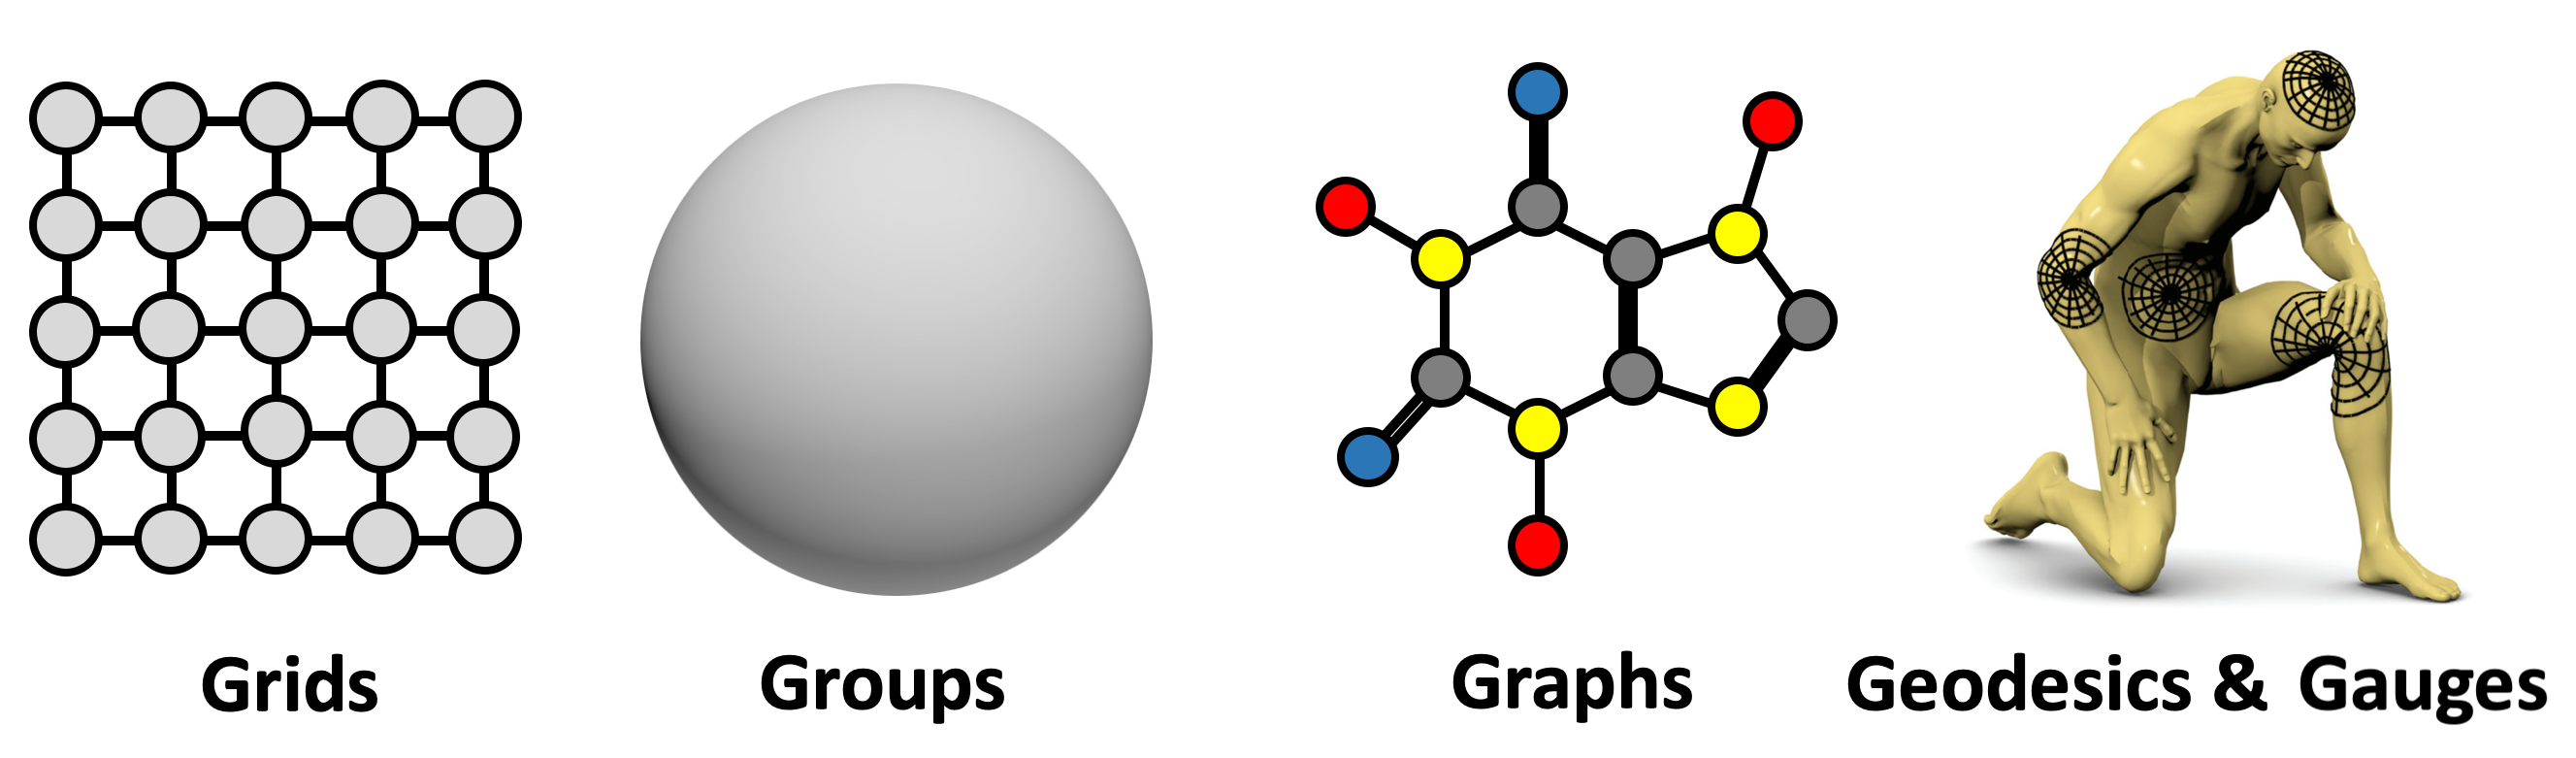
\includegraphics[width=1\textwidth]{figures/5g.png}
    \caption{The 5G of Geometric Deep Learning: grids, groups \& homogeneous spaces with global symmetry, graphs, geodesics \& metrics on manifolds, and gauges (frames for tangent or feature spaces). }
    \label{fig:4g}
\end{figure}





\subsection{Graphs and Sets}\label{sec:proto-graphs}

%\joan{This is a very nice intro. 
%Just one comment: it would be great to use the transition from sets to graphs to reinforce the scale aspect mentioned in the previous sections. Sets cannot be coarsened in non-trivial ways, while graphs can. 

%Another more general aspect that we need to nail in this section that clearly separates the graph treatment from, say the grid treatment: the domain varies with the input and thus becomes `part' of the input. I think again the transition from set to graph is useful here. The set is always the same geometric object modulo the change in size. The graph provides a new input to the system (as you say, via et its adjacency). 
%}





%\michael{\bf [MB: I took the liberty to rewrite this section making it less detailed and more `conversational' like the style of the previous sections in the Introduction chapter, anticipating that Chapter on graphs to be more rigorous.]}


%\joan{Joan: 
% Great detail and everything important seems to be here already. Two remarks:
% \begin{itemize}
%     \item I would frontload the section a bit more, explaining that we will first describe the domain, and then explain how the geometric priors and the blueprint are expressed.
%     \item Currently, this section re-derives the definitions of invariance/equivariance described previously, as well as the blueprint. I think it can be made shorter and more coherent to simply describe the two forms of group representation arising here (one for sets, and the other for graphs, where adjacency is also present), as well as the metric induced in the graph that is used to define local operators. 
%     \item In other words, I think these sections should derive the class of local linear equivariants for each symmetry group under consideration. In this section of sets and graphs, we should explain the two classes that arise (cf Maron et al.). 
%     \item The notation needs to be unified with the previous sections. 
%     
% \end{itemize}
%}

%\michael{MB: Agree in principle but we should not fall into the Bourbaki extreme. I suggest keep domain-specific notation to use familiar concepts and relate them to blueprint on the high level rather than in detail.

%I suggest to remove reference to particular models and talk about general concepts here. 
%}

In multiple branches of science, from sociology to particle physics, graphs are used as models of systems of relations and interactions. From our perspective, graphs give rise to a very basic type of invariance modelled by the group of permutations. 
Furthermore, other objects of interest to us, such as grids and sets, can be obtained as a particular case of graphs.  
%
%since graphs exhibit less restrictive geometries and invariances, they invite for the most flexible class of architectures---the \emph{Graph Neural Networks} (GNN). As we will see, all of the neural architectures we will study in this book can be understood as a special case of the GNN, with injected additional geometric constraints and invariances.


%the {\em symmetric group}), a . 


A {\em graph} $\gG = (\gV, \gE)$ is a collection of {\em nodes}\marginnote{Depending on the application field, nodes may also be called \emph{vertices}, and edges are often referred to as \emph{links} or \emph{relations}. We will use these terms interchangeably.} $\gV$  and {\em edges} $\gE \subseteq \gV\times \gV$ between pairs of nodes. For the purpose of the following discussion, we will further assume the nodes to be endowed with $s$-dimensional {\em node features}, 
denoted by $\mathbf{x}_u$ for all $u \in \gV$. 
%
Social networks are perhaps among the most commonly studied examples of graphs, where nodes represent users, edges correspond to friendship relations between them, and node features model user properties such as age, profile picture, etc. It is also often possible to endow the edges, or entire graphs, with features;\marginnote{
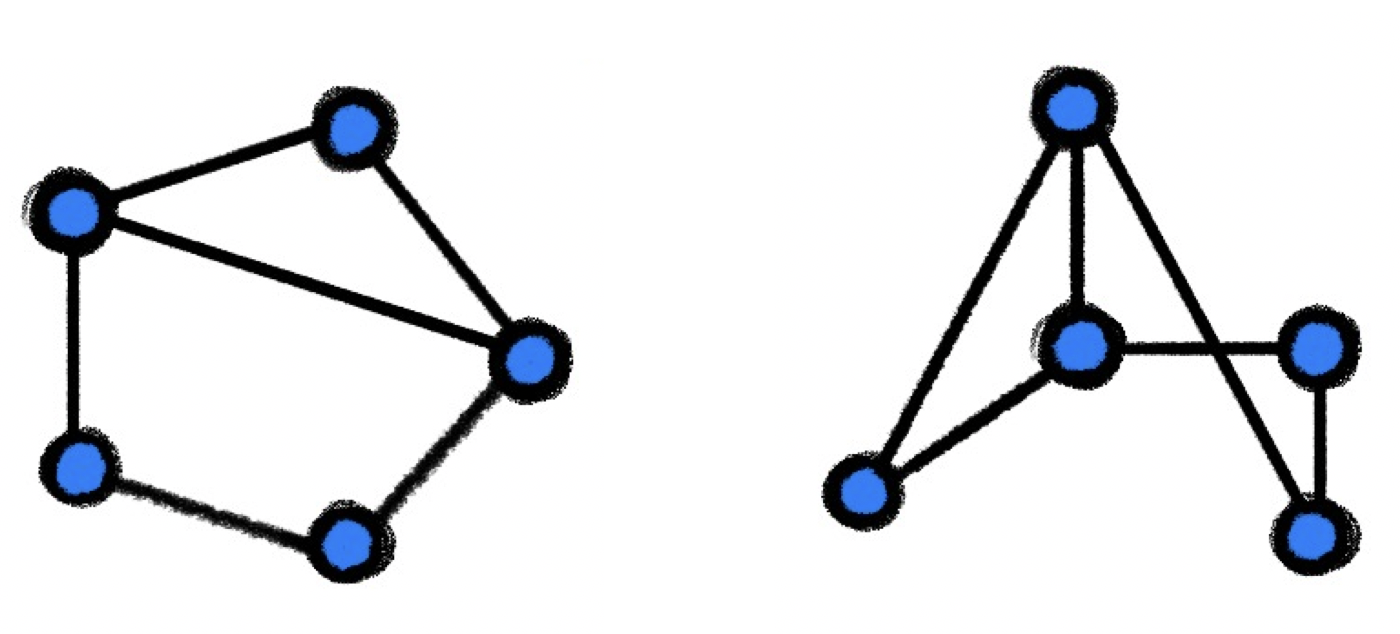
\includegraphics[width=0.8\linewidth]{figures/mn_isomorphic.png}
{\em Isomorphism} is an edge-preserving bijection between two graphs. Two isomorphic graphs shown here are identical up to reordering of their nodes. 
} but as this does not alter the main findings of this section, we will defer discussing it to future work.


The key structural property of graphs is that the nodes in $\gV$ are usually not assumed to be provided in any particular order, and thus any operations performed on graphs should not depend on the ordering of nodes. The desirable property  that functions acting on graphs should satisfy is thus {\em permutation invariance}, and it implies that for any two \emph{isomorphic} graphs,  the outcomes of these functions are identical. 
%
%
%This is clearly a 
We can see this as a 
particular setting of our blueprint, where the domain $\Omega = \mathcal{G}$ and the space $\mathcal{X}(\mathcal{G},\mathbb{R}^d)$ is that of $d$-dimensional node-wise signals. 
%
The symmetry we consider is given by the \emph{permutation group} $\mathfrak{G} = \Sigma_n$, whose elements are all the possible orderings of the set of node indices $\{1,\hdots, n\}$. 

%\michael{Harmonize notation: do we use $s$ or $d$ for dimension of features? } \joan{I am making a pass, using $s$ for feature dimension}\michael{we always used $d$, changing}

%In the language of the previous sections:\marginnote{However, we will almost always omit such notation for graphs, as they are assumed to be \emph{discrete} collections of nodes; hence, the language of linear algebra will admit higher notational simplicity.} for graphs we consider the input space to be defined on the domain  $\Omega = \mathcal{V}$, with the input space $\mathcal{X}(\mathcal{G}) = \{x : \mathcal{V}\rightarrow\mathbb{R}^s\}$ consisting of functions that attach node feature vectors to every node; $x(v) = \vec{x}_v$.
%\joan{Notation-wise: align with previous section $\Omega$ for domain, $\gX$ for signals over the domain} \michael{We use $x$ for signals, but $\Omega$ must be specific. }



%
%Accordingly, we focus on the permutation group actions $\frak{g}\in\frak{G}$ that permute the node ordering by applying such a matrix: $\frak{g}.{\bf X} = {\bf P}{\bf X}$. %


%$$ (where $n$ is the number of nodes).

%\begin{equation}
%    {\bf P}_{(2, 4, 1, 3)}{\bf X} =
%    \left[
%    \begin{array}{cccc}
%        0 & 1 & 0 & 0\\
%        0 & 0 & 0 & 1\\
%        1 & 0 & 0 & 0\\
%        0 & 0 & 1 & 0
%    \end{array}\right]\left[
%  \begin{array}{ccc}
%    \horzbar & \mathbf{x}_1 & \horzbar \\
%    \horzbar & \mathbf{x}_2 & \horzbar \\
%      \horzbar        &   \mathbf{x}_3  &    \horzbar       \\
%    \horzbar & \mathbf{x}_4 & \horzbar
%  \end{array}\right] = \left[\begin{array}{ccc}
%   \horzbar & \mathbf{x}_2 & \horzbar \\
%    \horzbar & \mathbf{x}_4 & \horzbar \\
 %     \horzbar        &   \mathbf{x}_1  &    \horzbar       \\
%    \horzbar & \mathbf{x}_3 & \horzbar
%  \end{array}\right]
%\end{equation}




%The first kind of object we will be studying is that of the \emph{graph}, which corresponds to the mother of all finite symmetry groups: the group of permutations. For the purposes of this chapter, we will define graphs as $G=(V, E)$, where $V$ is the set of \emph{nodes} and $E\subseteq V\times V$ is a set of \emph{edges} between pairs of nodes. For a commonly-studied example, social networks can be readily represented as graphs where nodes correspond to users, and edges correspond to the friendship links between them. 

%For now, we will assume that the graph's nodes are endowed with \emph{node features}, represented by $\mathcal{X} = \left\{\mathbf{x}_1, \mathbf{x}_2, \dots, \mathbf{x}_{|V|}\right\}$, where $\mathbf{x}_i\in\mathbb{R}^k$ are the features of node $i\in V$. In the social network analogy, these features could correspond to (some encoding of) the user's biography, interests or profile picture. Additional featurizations are possible, e.g. having features on the edges or entire graphs, but we will omit them for simplicity for now. 

%Compared with the subsequent objects, graphs exhibit less restrictive geometries and invariances, and hence invite for the most flexible class of architectures---the \emph{Graph Neural Networks} (GNN). Indeed, all of the neural architectures we will study can be understood as a special case of the GNN, with injected additional geometric constraints and invariances.

%The key structural property of graphs is that the nodes in $V$ are usually not assumed to be provided in any particular order, and thus any operations performed on graphs should not depend on the ordering of nodes. This desirable property that operations should satisfy is {\em permutation invariance}, and it implies that for any two \emph{isomorphic} graphs,\footnote{Isomorphism is an edge-preserving bijection between two graphs. Two isomorphic graphs are identical up to reordering of their nodes. } the outcomes of these operations are identical. 


Let us first illustrate the concept of permutation invariance on \emph{sets}, a special case of graphs without edges (i.e., $\gE=\emptyset$). 
%
By stacking the node features as rows of the $n\times d$ matrix
 $\mathbf{X} = (\mathbf{x}_1, \hdots, \mathbf{x}_n)^\top$, we do effectively specify an ordering of the nodes. 
 %
The action of the permutation $\mathfrak{g}\in\Sigma_n$ on  the set of nodes amounts to the reordering of the rows of $\mathbf{X}$, which can be represented as an $n\times n$ {\em permutation matrix} $\rho(\mathfrak{g}) = \mathbf{P}$,\marginnote{There are exactly $n!$ such permutations, so $\Sigma_n$ is, even for modest $n$, a very large group. } where each row and column contains exactly one $1$ and all the other entries are zeros. 



%  We may obtain a different ordering by applying an appropriate permutation matrix  $\mathbf{P}$,\marginnote{There are exactly $n!$ such permutations. } where each row and column contains exactly one $1$ and all the other entries are zeros. Accordingly, we focus on the permutation group actions $\frak{g}\in\frak{G}$ that permute the node ordering by applying such a matrix: $\frak{g}.{\bf X} = {\bf P}{\bf X}$. %
 
 %\begin{equation}
 %    a(\vec{x}, \vec{y}) = \left<\vec{W}\vec{x}, \vec{U}\vec{y}\right> \qquad a(\vec{x}, \vec{y}) = \vec{a}^\top({\bf Wx} + {\bf Uy})
 %\end{equation}
 
 %\begin{align*}
 %    {\bf x}^\top{\bf L}{\bf x} &= \frac{1}{2}\sum_{u\in\mathcal{V}}\sum_{v\in\mathcal{V}} a_{uv}(x_u - x_v)^2\\ &= \sum_{(u, v)\in\mathcal{E}} (x_u - x_v)^2
 %\end{align*}

 
 %, ${\bf P}\in\mathbb{R}^{|V|\times|V|}$, to ${\bf X}$. 
 


%Let ${\bf X}\in\mathbb{R}^{|V|\times k}$ be a \emph{node feature matrix} which is obtained by stacking $\mathbf{x}_i$ in a particular order. This effectively specifies one \emph{ordering} of this set of node features; we may obtain any different order by applying an appropriate permutation matrix, ${\bf P}\in\mathbb{R}^{|V|\times|V|}$, to ${\bf X}$. 
A function $f$ operating on this set is then said to be \emph{permutation invariant} if, for any such permutation matrix ${\bf P}$, it holds that $f({\bf P}{\bf X}) = f({\bf X})$. One simple such function is 
%, exploited by the Deep Sets model \citep{zaheer2017deep}, is
\begin{equation}
\label{eq:basicinv}
    f({\bf X}) = \phi\left(\sum_{u\in \gV} \psi\left(\mathbf{ x}_u\right)\right)~,
\end{equation}
where the function $\psi$ is independently applied to every node's features, and $\phi$ is applied on its \emph{sum-aggregated} outputs: as sum is independent of the order in which its inputs are provided, such a function is  invariant with respect to the permutation of the node set, and is hence guaranteed to always return the same output, no matter how the nodes are permuted.

%\michael{Notation: should we use $\mathbf{f}(\mathbf{X})$ since the output can be a vector?}
%\petar{I would tend to stick with the $f$ notation}

 
%node features in $\mathcal{X}$ are permuted.



Functions like the above provide a `global' graph-wise output, but very often, we will be interested in functions that act `locally', in a node-wise manner. 
%return more fine-grained information. 
For example, we may want to apply some function to \emph{update} the features in every node, obtaining the set of \emph{latent} node features. 
%, $\mathbf{h}_1, \hdots, \mathbf{h}_n$. 
%$\mathcal{H}=\left\{\mathbf{h}_1, \mathbf{h}_2, \dots, \mathbf{h}_{|V|}\right\}$.
%
%Strictly speaking, 
If we stack these latent features into a matrix $\mathbf{H} = \mathbf{F}({\bf X})$\marginnote{We use the bold notation  for our function $\mathbf{F}(\mathbf{X})$ to emphasise it outputs node-wise vector features and is hence a matrix-valued function.} is no longer permutation invariant: the order of the rows of ${\bf H}$ should be \emph{tied} to the order of the rows of ${\bf X}$, so that we know which output node feature corresponds to which input node. We need instead  a more fine-grained notion of {\em permutation equivariance}, stating that, once we ``commit'' to a permutation of inputs, it consistently permutes the resulting objects. 
%
Formally, $\mathbf{F}(\mathbf{X})$ is a \emph{permutation equivariant} function if, for any permutation matrix ${\bf P}$, it holds that $\mathbf{F}({\bf P}{\bf X}) = {\bf P}\mathbf{F}({\bf X})$. A shared node-wise linear transform 
\begin{equation}
    \mathbf{F}_{\mathbf\Theta}({\bf X}) = {\bf X}{\mathbf \Theta}
    %\qquad \text{, i.e.,} \qquad {\vec h}_i = {\mathbf\Theta}^T\mathbf{x}_i
\end{equation}
specified by a weight matrix $\mathbf\Theta\in\mathbb{R}^{d\times d'}$, is one possible construction of such a permutation equivariant function, producing in our example 
latent features of the form 
$\mathbf{h}_u = \boldsymbol{\Theta}^\top\mathbf{x}_u$.
%\joan{This is very clear and nicely explained, but it is a particular case of the group equivariance discussion from previous section. I would add a pointer at the beginning or the end of this paragraph to tie things together. Upps just saw the following paragraph, nevermind. }

%\michael{Notation: do we use $h$ or $y$ for output?}
%\petar{$h$ for what comes out of an equivariant layer; the assumption is that we can stack more than one, or even attach invariant tail, to get a desirable $y$ (which should maybe be reserved for downstream task outputs?).}


%In fact, the construction from Equation (\ref{eq:basicinv}) arises naturally from the GDL blueprint. 
This construction arises naturally from our Geometric Deep Learning blueprint. 
We can first attempt to characterise {\em linear equivariants} (functions of the form $\mathbf{F} {\bf P X} = \bf{P} \mathbf{FX}$), for which it is easy to verify 
that any such map can be written as a linear combination of two \emph{generators}, the identity $\mathbf{F}_1 \mathbf{X} = {\bf X}$ and the average ${\mathbf{F}_2 \mathbf{X}}= \frac{1}{n}\boldsymbol{1}\boldsymbol{1}^\top \mathbf{X} = \frac{1}{n} \sum_{u=1}^n {\bf x}_u$. As will be described in Section \ref{sec:deepset}, the popular Deep Sets \citep{zaheer2017deep} architecture follows precisely this blueprint.
%\joan{Remark to avoid confusion that $\mathbf{X}$ here should be understood as a vector, not a matrix}


% TODO: explain relation to representations & equivariance as explained in previous section.
% Invariant features correspond to a trivial representation
% Node features correspond to rho(P) = P
% Edge features / adjacency matrix corresponds to rho(P) = P tensor P.


We can now generalise the notions of permutation invariance and equivariance from sets to graphs. 
%
In the generic setting $\gE\neq\emptyset$, the graph connectivity can be represented by the $n\times n$ {\em adjacency matrix} $\mathbf{A}$,\marginnote{When the graph is {\em undirected}, i.e. $(u,v) \in \gE$ iff $(v,u) \in \gE$, the adjacency matrix is {\em symmetric}, $\mathbf{A}= \mathbf{A}^\top$. } defined as  
\begin{equation}
    a_{uv} = \begin{cases}
    1 & (u, v)\in \gE\\
    0 & \text{otherwise}.
    \end{cases}
\end{equation}
%
Note that now the adjacency and feature matrices $\mathbf{A}$ and $\mathbf{X}$ are ``synchronised'', in the sense that $a_{uv}$ specifies the adjacency information between the nodes described by the $u$th and $v$th rows of $\mathbf{X}$. Therefore, applying a permutation matrix $\mathbf{P}$ to the node features $\mathbf{X}$ automatically implies applying it to $\mathbf{A}$'s rows and columns, $\mathbf{P}\mathbf{A}\mathbf{P}^\top$. \marginnote{$\mathbf{P}\mathbf{A}\mathbf{P}^\top$ is the representation of $\Sigma_n$ acting on matrices. }
%
%
We say that (a graph-wise function) $f$ is \emph{permutation invariant} if  
\begin{equation}
f({\bf PX}, {\bf PAP}^\top) = f({\bf X}, {\bf A})\marginnote{As a way to emphasise the fact that our functions operating over graphs now need to take into account the adjacency information, we use the notation $f({\bf X}, {\bf A})$.}
\end{equation}
and (a node-wise function) $\mathbf{F}$ is \emph{permutation equivariant} if 
\begin{equation}
\label{eq:permequivgraph}
\mathbf{F}({\bf PX}, {\bf PAP}^\top) = {\bf P}\mathbf{F}({\bf X}, {\bf A})
\end{equation}
for any permutation matrix  ${\bf P}$.
%
%
%\taco{Taco: should we relate this to the blueprint? We can mention here that $PX$ and $PAP^T$ are examples of representations of the permutation group. We can then go on to say that the graph structure tells us which nodes are close in a certain sense, and that most graph nets exploit this, leading into the next paragraph.}\michael{I do say above that $\rho(\fg)=P$}
%
%Armed with the concepts of permutation invariance and equivariance, we can consider a generic graph connectivity setup, where $E\neq\emptyset$. One typical way to represent this adjacency information in a compact form is the \emph{adjacency matrix}, ${\bf A}\in\mathbb{R}^{|V|\times|V|}$, which is in the simplest case (of an unweighted and undirected graph), a binary and symmetric matrix; that is:
%\begin{equation}
%    {\bf A}_{ij} = {\bf A}_{ji} = \begin{cases}
%    1 & (i, j)\in E\\
%    0 & \text{otherwise}
%    \end{cases}
%\end{equation}
%
%
%We can now generalise the notions of permutation invariance and equivariance from sets to graphs. We note that the order of the rows and columns in ${\bf A}$ is constrained to respect the order of the rows of ${\bf X}$---that is, ${\bf A}_{ij}$ specifies the adjacency information between the nodes described by the $i$-th and $j$-th row of ${\bf X}$. Then, applying a permutation matrix ${\bf P}$ to the nodes in ${\bf X}$ automatically implies applying it to ${\bf A}$'s rows and columns, yielding ${\bf P}{\bf A}{\bf P}^T$. 


%Following again the Geometric Deep Learning blueprint, 
Here again, we can first characterise linear equivariant functions.\marginnote{This corresponds to the {\em Bell number} $B_4$, which counts the number of ways to partition a set of $4$ elements, in this case given by the 4-indices $(u,v), (u',v')$ indexing a linear map acting on the adjacency matrix.  %\cite{maron2018invariant}.
}  
As observed by \cite{maron2018invariant}, any linear $\mathbf{F}$ satisfying equation (\ref{eq:permequivgraph}) can be expressed as a linear combination 
of fifteen linear generators; remarkably, this family of generators is {\em independent of} $n$. 
%
%
%
Amongst these generators, our blueprint specifically advocates for those that are also {\em local}, i.e., whereby  
the output on node $u$ directly depends on its neighbouring nodes in the graph. We can formalise this constraint explicitly in our model construction, by defining what it means for a node to be neighbouring another.



A (undirected) {\em neighbourhood} of node $u$, sometimes also called {\em 1-hop},  is defined as \marginnote{
%Our definition of neighbourhood does not account for directed edges. 
Often, the node $u$ itself is included in its own neighbourhood.}
\begin{equation}
    \mathcal{N}_u = \{ v : (u,v) \in \gE \,\mathrm{or}\, (v,u) \in \gE \}
    %\left\{j\ |\ i=j\vee {\bf A}_{ij} = 1\right\}
\end{equation}
%
and the {\em neighbourhood features} as the multiset 
%
\begin{equation}
    \mathbf{X}_{\mathcal{N}_u} = \ldblbrace \mathbf{x}_v : v\in\mathcal{N}_u \rdblbrace.
\marginnote{A {\em multiset}, denoted $\ldblbrace \, \dots \, \rdblbrace$, is a set where the same element can appear more than once. This is the case here because the features of different nodes can be equal.}
\end{equation}
%%
Operating on 1-hop neighbourhoods aligns well with the \emph{locality} aspect of our blueprint: namely, defining our metric over graphs as the \emph{shortest path distance} between nodes using edges in $\mathcal{E}$.% \michael{I suggest we get rid of this, since we never talked about metrics in a rigorous way. } \petar{There seems to still be a discussion of a metric when defining locality in the blueprint---this is what I was referring to. I think it's fine as-is, but wouldn't mind removing it.} \joan{I think mentioning it qualitatively like this is fine, it conveys an important message}
%Processing 1-hop neighbourhoods over graphs exactly corresponds with defining our metric over graphs, $g$, as the \emph{shortest path distance} between nodes using edges in $\mathcal{E}$, and setting $\delta = 1$.

%This also closely aligns with the \emph{locality} condition of the main building block of our geometric deep learning blueprint. Processing 1-hop neighbourhoods over graphs exactly corresponds with defining our metric over graphs, $g$, as the \emph{shortest path distance} between nodes using edges in $\mathcal{E}$, and setting $\delta = 1$.

%
The GDL blueprint thus yields a general recipe for constructing permutation equivariant functions on graphs, by specifying a \emph{local} function $\phi$ that operates over the features of a node and its neighbourhood, $\phi(\mathbf{x}_u, \mathbf{X}_{\mathcal{N}_u})$. Then, a permutation equivariant function $\mathbf{F}$ can be constructed by applying $\phi$ to every node's neighbourhood in isolation (see Figure \ref{fig:gc_gdl}):
\begin{equation}
    \mathbf{F}({\bf X}, {\bf A}) =
\left[
  \begin{array}{ccc}
    \horzbar & \phi(\mathbf{x}_1, \mathbf{X}_{\mathcal{N}_1}) & \horzbar \\
    \horzbar & \phi(\mathbf{x}_2, \mathbf{X}_{\mathcal{N}_2}) & \horzbar \\
             & \vdots    &          \\
    \horzbar & \phi(\mathbf{x}_n, \mathbf{X}_{\mathcal{N}_n}) & \horzbar
  \end{array}
\right]
\label{eq:graph_equivariant}
\end{equation}
As $\mathbf{F}$ is constructed by applying a shared function $\phi$ to each node locally, its permutation equivariance rests on $\phi$'s output being independent on the ordering of the nodes in $\mathcal{N}_u$. Thus, if $\phi$ is built to be permutation invariant, then this property is satisfied.
%
As we will see in future work, the choice of $\phi$ plays a crucial role in the expressive power of such a  scheme. When $\phi$ is injective, it is equivalent to one step of the {\em Weisfeiler-Lehman graph isomorphism test}, a classical algorithm in graph theory providing a necessary condition for two graphs to be isomorphic by an iterative color refinement procedure. 


%\michael{ADD: geometric stability of graph filters}

%We conclude our introduction with a discussion on how to generally construct useful functions over graphs that are permutation equivariant. A function over graphs is likely to be useful if it directly exploits the structure present in ${\bf A}$---that is, if outputs on node $i$ directly depend on its \emph{neighbouring} nodes in the graph (e.g. the non-zero entries of $\mathbf{a}_i$ and $\mathbf{a}_i^T$).

%From this concept, we can define a \emph{neighbourhood} of node $i$ in the graph, commonly denoted as $\mathcal{N}_i$, to include all first-order neighbours of $i$, often including $i$ itself:
%\begin{equation}
%    \mathcal{N}_i = \left\{j\ |\ i=j\vee {\bf A}_{ij} = 1\right\}
%\end{equation}
%Accordingly, we can define the set of \emph{neighbourhood features} of $i$, $\mathbf{X}_{\mathcal{N}_i}\in\mathcal{P}(\mathbb{R}^k)$:
%\begin{equation}
%    \mathbf{X}_{\mathcal{N}_i} = \left\{\mathbf{x}_j\ |\ j\in\mathcal{N}_i\right\}
%\end{equation}
\begin{figure}
    \centering
    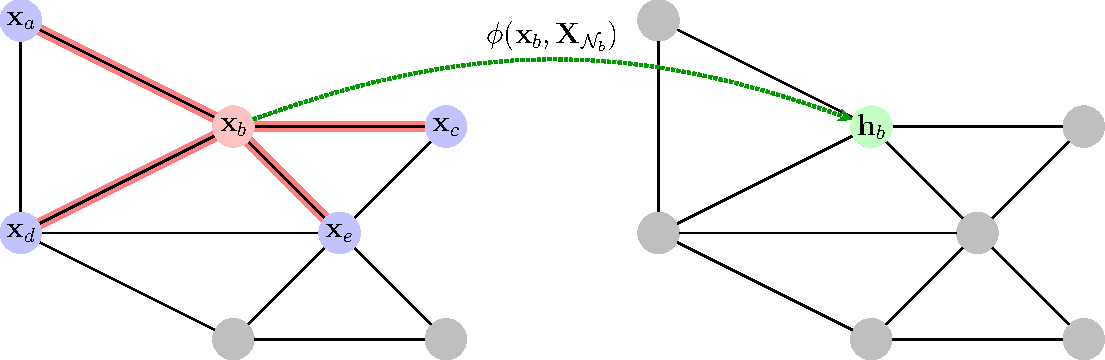
\includegraphics[width=\linewidth]{figures/GC_GDL.pdf}
    \caption{An illustration of constructing permutation-equivariant functions over graphs, by applying a permutation-invariant function $\phi$ to every neighbourhood. In this case, $\phi$ is applied to the features $\mathbf{x}_b$ of node $b$ as well as the multiset  of its neighbourhood features, $\mathbf{X}_{\mathcal{N}_b} = \ldblbrace\mathbf{x}_a, \mathbf{x}_b, \mathbf{x}_c, \mathbf{x}_d, \mathbf{x}_e\rdblbrace$. Applying $\phi$ in this manner to every node's neighbourhood recovers the rows of the resulting matrix of latents features $\mathbf{H}=\mathbf{F}(\mathbf{X}, \mathbf{A})$.}
    \label{fig:gc_gdl}
\end{figure}%
%\michael{\bf [MB: shall we use the notation of multisets here?]}


%The general concept of constructing {\em permutation equivariant} functions operating over graphs as shared {\em permutation invariant} functions operating over local neighbourhoods appears to be very powerful and underlies the design of most Graph Neural Networks. Under various guises, this local function $g$ can be referred to as ``diffusion'', ``propagation'', or ``message passing''. 
%
%If we are interested in a graph-level output, a common recipe is to construct the latent node features using a {\em permutation equivariant} function $f$, followed by a {\em permutation invariant} function $h$ over the entries of $f({\bf X}, {\bf A})$ to obtain an ordering-independent output. In this context, the function $h$ is often referred to as ``readout'' or ``global pooling''.

%Motivation: examples from 
%- Images, Text, Speech. 
%- Social Networks
%- Physical Sciences
%- Chemistry and medicine
%- 3D Computer vision and Graphics


%Finally, 
It is also worth noticing that the difference between functions defined on sets and more general graphs in this example is that in the latter case we need to explicitly account for the structure of the domain. 
%
As a consequence, graphs stand apart in the sense that the domain becomes {\em part of the input} in machine learning problems, whereas when dealing with sets and grids (both particular cases of graphs) we can specify only the features and assume the domain to be {\em fixed}. 
%
This distinction will be a recurring motif in our discussion. 
%
As a result, the notion of geometric stability (invariance to domain deformation) is crucial in most problems of learning on graphs. It straightforwardly follows from our construction that permutation invariant and equivariant functions produce identical outputs on isomorphic (topologically-equivalent) graphs. These results can be generalised to approximately isomorphic graphs, and several results on stability under graph perturbations exist  \citep{levie2018cayleynets}.  We will return to this important point in our discussion on manifolds, which we will use as an vehicle to study such invariance in further detail. 


Second, due to their additional structure, graphs and grids, unlike sets, can be coarsened in a non-trivial way\marginnote{More precisely, we cannot define a non-trivial coarsening assuming set structure alone. There exist established approaches that infer topological structure from unordered sets, and those can admit non-trivial coarsening.}, giving rise to a variety of pooling operations. 
%These will also be covered within Chapter \ref{ch:graphs}. 
%
%Finally, 



\subsection{Grids and Euclidean spaces} 
\label{sec:grids_euclidean}

%\joan{Joan: Good section; perhaps we could shrink a bit by removing the repetitive parts between blueprint, discrete and then continuous case. Also further highlight the fundamental differences between grids and graphs in terms of group representation (permutation group vs translation group, one-parameter group in one case), and geometry (homogeneous vs non-homogeneous): consequences in terms of global orientation, etc. 
%}
%\michael{This more naturally comes after the Groups section, was a natural transition to manifolds which are non-homogeneous}

%images, CNNs, RNNs

The second type of objects we consider are grids. 
%
It is fair to say that the impact of deep learning was particularly dramatic in computer vision,  natural language processing, and speech recognition. These applications all share a %an essential 
geometric common denominator: an underlying grid structure. 
%translation invariance/equivariance, alongside scale separation. 
%
As already mentioned, grids are a particular case of graphs with special adjacency. However, since the order of nodes in a grid is fixed, machine learning models for signals defined on grids are no longer required to account for permutation invariance, and have a stronger geometric prior: translation invariance. 
%can be designed to leverage the translation invariance prior. 

%This gives rise to powerful and efficient deep learning architectures---{\em Convolutional Neural Networks} (CNNs). 



\paragraph{Circulant matrices and Convolutions}
Let us dwell on this point in more detail. 
Assuming for simplicity periodic boundary conditions, we can think of a one-dimensional grid as a {\em ring graph}\marginnote{
    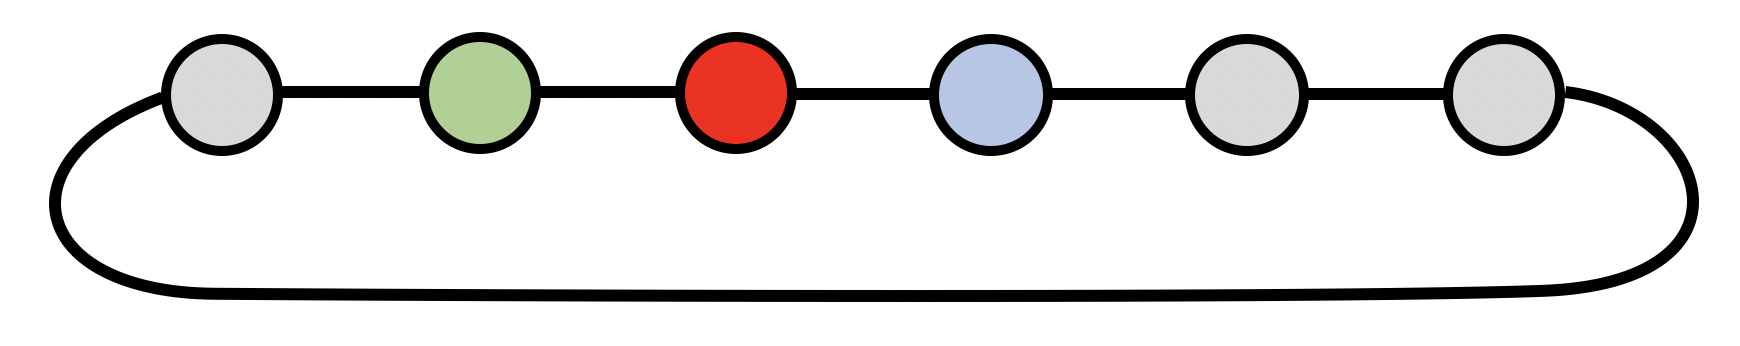
\includegraphics[width=0.9\linewidth]{figures/grid.png}
} with nodes indexed by $0, 1,\hdots, n-1$ modulo $n$ (which we will omit for notation brevity) and
the adjacency matrix with elements $a_{u,u+1 \, \mathrm{mod} \, n} = 1$ and zero otherwise. There are two main differences from the general graph case we have discussed before. 
%
First, each node $u$ has identical connectivity, to its neighbours $u-1$ and $u+1$, and thus structure-wise indistinguishable from the others. 
%in terms of group theory, we say that the grid is a homogeneous space. 
\marginnote{As we will see later, this makes the grid a homogeneous space.
  %  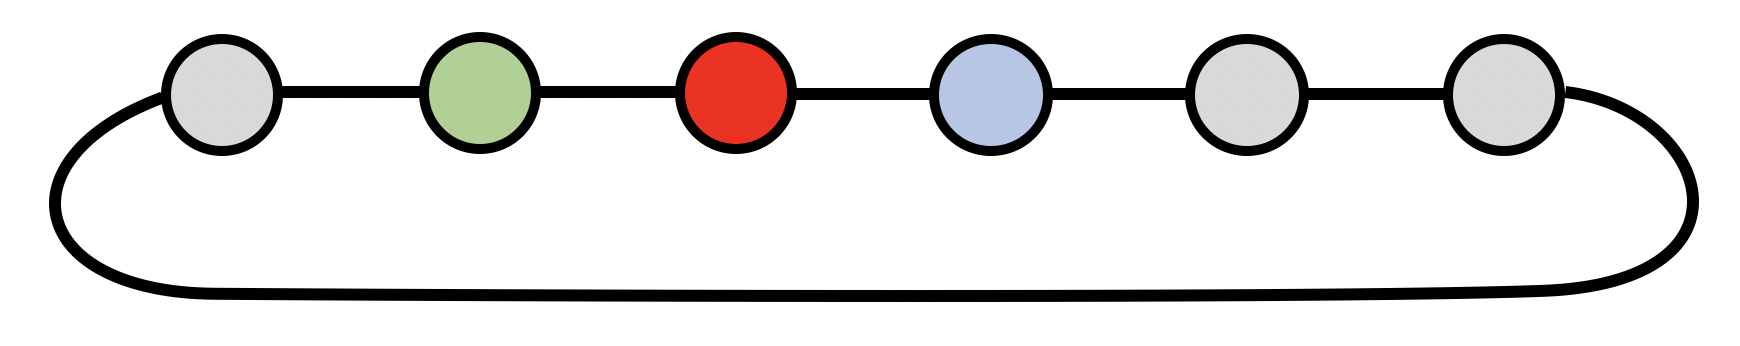
\includegraphics[width=1\linewidth]{figures/grid.png}
}
%
Second and more importantly, since the nodes of the grid have a fixed ordering, we also have a fixed ordering of the {\em neighbours:} we can call $u-1$ the `left neighbour' and $u+1 $ the `right neighbour'.
%
If we use our previous recipe for designing a equivariant function $\mathbf{F}$ using a local aggregation function $\phi$, we now have $\mathbf{f}(\mathbf{x}_u) = \phi(\mathbf{x}_{u-1}, \mathbf{x}_{u}, \mathbf{x}_{u+1})$ at every node of the grid: $\phi$ does not need to be permutation invariant anymore.  
%
%
For a particular choice of a linear transformation $\phi(\mathbf{x}_{u-1}, \mathbf{x}_{u}, \mathbf{x}_{u+1}) = \theta_{-1}\mathbf{x}_{u-1} + \theta_0 \mathbf{x}_{u} + \theta_1 \mathbf{x}_{u+1}$, we can write $\vec{F}(\mathbf{X})$ as a matrix product, 
$$
\vec{F}(\mathbf{X}) = 
\left[
\begin{array}{ccccc}
\theta_0 & \theta_1  & & & \theta_{-1}\\
 \theta_{-1} & \theta_0 & \theta_1 & & \\
&  \ddots & \ddots & \ddots & \\
 &  & \theta_{-1} & \theta_0 & \theta_1\\
\theta_1 &  &  & \theta_{-1} & \theta_0

 \end{array}
  \right]
  %
\left[  
    \begin{array}{ccc}
    \horzbar & \mathbf{x}_0 & \horzbar \\
    \horzbar & \mathbf{x}_1 & \horzbar \\
             & \vdots    &          \\
    \horzbar & \mathbf{x}_{n-2} & \horzbar  \\           
    \horzbar & \mathbf{x}_{n-1} & \horzbar
  \end{array}
   \right]
$$
%
Note this very special multi-diagonal structure with one element repeated along each diagonal, sometimes referred to as ``weight sharing'' in the machine learning literature. 
%
%In machine learning literature, it is sometimes referred to as %``weight sharing'', a prominent feature of CNNs where the same %weights are applied at different positions in an image. 

%\michael{Notation: we denoted filters by $\theta$}

More generally, given a vector $\boldsymbol{\theta} = (\theta_0, \hdots, \theta_{n-1})$, a {\em circulant matrix} 
$\mathbf{C}(\boldsymbol{\theta}) = (\theta_{u-v \, \mathrm{mod} \, n})$ is obtained by appending circularly shifted versions of the vector $\boldsymbol{\theta}$.  
%
Circulant matrices are synonymous with discrete convolutions, \marginnote{Because of the periodic boundary conditions, it is a {\em circular} or {\em cyclic convolution}. In signal processing, $\boldsymbol{\theta}$ is often referred to as the ``filter,'' and in CNNs, its coefficients are learnable. } 
%\taco{TODO: change this equation to a cross-correlation, and add a note saying that technically this is called a cc but we'll call it a conv.}
$$
(\mathbf{x} \star \boldsymbol{\theta})_u = \sum_{v=0}^{n-1}  x_{v \, \mathrm{mod}\, n} \,\, \theta_{u-v \, \mathrm{mod}\, n}
$$
%
as one has $\mathbf{C}(\boldsymbol{\theta})\mathbf{x} = \mathbf{x} \star \boldsymbol{\theta}$. 
%\petar{Should $i$ be replaced with $u$ in the equation above, given our blueprint? I did this in the CNN section.}
%
A particular choice of $\boldsymbol{\theta}=(0,1,0,\hdots, 0)^\top$ yields a special circulant matrix that shifts vectors to the right by one position. This matrix is called the (right) {\em shift} or {\em translation operator}  and denoted by $\mathbf{S}$.\marginnote{The left shift operator is given by $\mathbf{S}^\top$. Obviously, shifting left and then right (or vice versa) does not do anything, which means $\mathbf{S}$ is {\em orthogonal}: $\mathbf{S}^\top \mathbf{S} = \mathbf{S} \mathbf{S}^\top = \mathbf{I}$.} 


%\michael{Notation: Replace $T$ by $S$}


%\michael{Naming: shift vs translation}


Circulant matrices can be characterised by their {\em commutativity} property: the product of circulant matrices is commutative, i.e. 
$\mathbf{C}(\boldsymbol{\theta}) \mathbf{C}(\boldsymbol{\eta}) = \mathbf{C}(\boldsymbol{\eta}) \mathbf{C}(\boldsymbol{\theta})$ for any $\boldsymbol{\theta}$ and $\boldsymbol{\eta}$.
%
Since the shift is a circulant matrix, we get the familiar {\em translation} or {\em shift equivariance} of the convolution operator, 
$$
\mathbf{S} \mathbf{C}(\boldsymbol{\theta}) \mathbf{x} = 
\mathbf{C}(\boldsymbol{\theta}) \mathbf{S} \mathbf{x}.
$$
%
Such commutativity property should not be surprising, since the underlying symmetry group (the translation group) is Abelian. 
Moreover, the opposite direction appears to be true as well, i.e. 
a matrix is circulant iff it commutes with shift.
%
This, in turn, allows us to {\em define} convolution as a translation equivariant linear operation, and is a nice illustration of the power of geometric priors and the overall philosophy of Geometric ML: convolution emerges from the first principle of translational symmetry. 


Note that unlike the situation on sets and graphs, the number of linearly independent shift-equivariant functions (convolutions) \emph{grows} with the size of the domain (since we have one degree of freedom in each diagonal of a circulant matrix). However, the scale separation prior guarantees filters can be {\em local}, resulting in the same $\Theta(1)$-parameter complexity per layer, as we will verify in Section \ref{sec:cnnsec} when discussing the use of these principles in the implementation of Convolutional Neural Network architectures.

%\joan{Link to GDL blueprint: 
%Convolutions also emerge as the essential device to build stable translation invariant representations, by querying the GDL blueprint. 
%Remark that, as opposed to the permutation group in sets and graphs, the number of linearly independent convolution maps \emph{grows} with the size of the domain (since we have one degree of freedom in each diagonal of a circulant matrix). However, the scale separation prior imposes only local filters, resulting in the same $\Theta(1)$-parameter complexity per layer, as we will verify in Section \ref{sec:cnnsec}.  }



\paragraph{Derivation of the discrete Fourier transform}
We have already mentioned the Fourier transform and its connection to convolution: the fact that the Fourier transform diagonalises the convolution operation is an important property used in signal processing to perform convolution in the frequency domain as an element-wise product of the Fourier transforms. 
%
However, textbooks usually only state this fact, rarely explaining {\em where} the Fourier transform comes from and what is so {\em special} about the Fourier basis. 
%
Here we can show it, demonstrating once more how foundational are the basic principles of symmetry. 


For this purpose, recall a fact from linear\marginnote{We must additionally assume distinct eigenvalues, otherwise there might be multiple possible diagonalisations. This assumption is satisfied with our choice of $\mathbf{S}$.}  algebra that (diagonalisable) matrices are {\em joinly diagonalisable} iff they mutually commute. 
%
In other words, there exists a common eigenbasis for all the circulant matrices, in which they differ only by their eigenvalues. 
%
We can therefore pick one circulant matrix and compute its eigenvectors---we are assured that these will be the eigenvectors of all other circulant matrices as well.
%\taco{I think this is true only if all eigenvalues of this matrix are distinct. Take e.g. the identity matrix, which is circulant, and can be (re-)diagonalized by any orthogonal matrix. Using the shift operator is fine in this respect}\michael{The statement here is on the existence of a joint diagonalization. True, some circulant matrices have different bases diagonalizing them, but not all of them will diagonalize other matrices. }
It is convenient to pick the shift operator, for which the eigenvectors happen to be the discrete Fourier basis \marginnote{
$\mathbf{S}$ is orthogonal but non-symmetric, hence, its eigenvectors are orthogonal but the eigenvalues are complex (roots of unity). 
}
$$
\boldsymbol{\varphi}_k = \frac{1}{\sqrt{n}}\left (1, e^{ \frac{2\pi \mi k}{n}}, e^{ \frac{4\pi \mi k}{n} }, \hdots , e^{ \frac{2\pi \mi  (n-1)k}{n} }
\right)^\top, \hspace{5mm} k = 0, 1, \hdots, n-1,  
$$
%
which we can arrange into an $n\times n$ Fourier matrix $\boldsymbol{\Phi} = (\boldsymbol{\varphi}_0, \hdots, \boldsymbol{\varphi}_{n-1})$.
% 
%
Multiplication by $\boldsymbol{\Phi}^*$\marginnote{Note that the eigenvectors are complex, so we need to take complex conjugation when transposing $\boldsymbol{\Phi}$.} 
gives the Discrete Fourier Transform (DFT), and by $\boldsymbol{\Phi}$ the inverse DFT, 
$$
\hat{x}_k = \frac{1}{\sqrt{n}}\sum_{u = 0}^{n-1}x_u e^{-\frac{2\pi \mi k u}{n} } \hspace{15mm}
%
{x}_u = \frac{1}{\sqrt{n}} \sum_{k = 0}^{n-1}\hat{x}_k e^{+\frac{2\pi \mi k u}{n} }.
$$

 
 
Since all circulant matrices are jointly diagonalisable,\marginnote{
Since the Fourier transform is an orthogonal matrix ($\boldsymbol{\Phi}^* \boldsymbol{\Phi} = \mathbf{I}$), geometrically it acts as a change of the system of coordinates that amounts to an $n$-dimensional rotation. In this system of coordinates (``Fourier domain''), the action of a circulant $\mathbf{C}$ matrix becomes element-wise product.
}  
they are also diagonalised by the Fourier transform 
and differ only in their eigenvalues. Since the eigenvalues of the circulant matrix $\mathbf{C}(\boldsymbol{\theta})$ are the Fourier transform of the filter (see e.g. \cite{bamieh2018discovering}), $\hat{\boldsymbol{\theta}} = \boldsymbol{\Phi}^* \boldsymbol{\theta}$, we obtain the Convolution Theorem: 
$$
\mathbf{C}(\boldsymbol{\theta}) \mathbf{x} = \boldsymbol{\Phi}
\left[  
    \begin{array}{ccc}
    \hat{\theta}_0 &  &  \\
    & \ddots & \\
    & & \hat{\theta}_{n-1}
  \end{array}
   \right]\boldsymbol{\Phi}^*\mathbf{x}
   = \boldsymbol{\Phi} (\hat{\boldsymbol{\theta}} \odot \hat{\mathbf{x}} )
$$
%

Because the Fourier matrix $\boldsymbol{\Phi}$ has a special algebraic structure, the products $\boldsymbol{\Phi}^\star \mathbf{x}$ and $\boldsymbol{\Phi} \mathbf{x}$ can be computed with $\mathcal{O}(n \log n)$ complexity using a Fast Fourier Transform (FFT) algorithm. This is one of the reasons why frequency-domain filtering is so popular in signal processing; furthermore, the filter is typically designed directly in the frequency domain, so the Fourier transform $\hat{\boldsymbol{\theta}}$ is never explicitly computed.


Besides the didactic value of the derivation of the Fourier transform
and convolution we have done here, it provides a scheme to generalise these concepts to graphs. Realising that the adjacency matrix of the ring graph is exactly the shift operator, one can can develop the graph Fourier transform and an analogy of the convolution operator by computing the eigenvectors of the adjacency matrix (see e.g. \cite{sandryhaila2013discrete}).
%
Early attempts to develop graph neural networks by analogy to CNNs, sometimes termed `spectral GNNs', exploited this exact blueprint.\marginnote{In graph signal processing, the eigenvectors of the {\em graph Laplacian} are often used as an alternative of the adjacency matrix to construct the graph Fourier transform, see \cite{shuman2013emerging}. On grids, both matrices have joint eigenvectors, but on graphs they results in somewhat different though related constructions.} 
%
We will see in %Chapter~\ref{ch:graphs} 
Sections~\ref{sec:manifolds}--\ref{sec:meshes}
that this analogy has some important limitations. 
%
The first limitation comes from the fact that a grid is fixed, and hence all signals on it can be represented in the same Fourier basis. In contrast, on general graphs, the Fourier basis depends on the structure of the graph. Hence, we cannot directly compare Fourier transforms on two different graphs --- a problem that translated into a lack of generalisation in machine learning problems. 
%
Secondly, multi-dimensional grids, which are constructed as tensor products of one-dimensional grids, retain the underlying structure: the Fourier basis elements and the corresponding frequencies (eigenvalues) can be organised in multiple dimensions. In images, for example, we can naturally talk about horizontal and vertical frequency and filters have a notion of {\em direction}. On graphs, the structure of the Fourier domain is one-dimensional, as we can only organise the Fourier basis functions by the magnitude of the corresponding frequencies. As a result, graph filters are oblivious of direction or {\em isotropic}. 



\paragraph{Derivation of the continuous Fourier transform}
For the sake of completeness, and as a segway for the next discussion, we repeat our analysis in the continuous setting. 
Like in Section~\ref{sec:scale_separation}, consider functions defined on $\Omega = \mathbb{R}$ and the translation operator $(S_v f)(u) = f(u-v)$ shifting $f$ by some position $v$. 
 %
 Applying $S_v$ to the Fourier basis functions $\varphi_\xi(u) = e^{\mi \xi u}$  yields, by associativity of the exponent,  
% \michael{Notation: same $\phi$ used to denote basis functions, filters, and local aggregators}
$$
S_v e^{\mi\xi u} = e^{\mi\xi (u-v)} = e^{-\mi\xi v} e^{\mi\xi u},
$$
i.e., $\varphi{u}_\xi(u)$ is the complex eigenvector of $S_v$ with the complex eigenvalue  $e^{-\mi\xi v} $ -- exactly mirroring the situation we had in the discrete setting. 
Since $S_v$ is a unitary operator (i.e., $\| S_v x \|_p = \| x \|_p$ for any $p$ and $x \in L_p(\R)$), any eigenvalue $\lambda$ must satisfy $|\lambda|=1$, which corresponds precisely to the eigenvalues $e^{-i\xi v}$ found above. 
Moreover, the spectrum of the translation operator is \emph{simple}, meaning that two functions sharing the same eigenvalue must necessarily be collinear. Indeed, suppose that $S_v f = e^{-\mi \xi_0 v} f$ for some $\xi_0$. Taking the Fourier transform in both sides, we obtain 
$$\forall ~\xi~,~e^{-\mi \xi v} \hat{f}(\xi) = e^{-\mi \xi_0 v} \hat{f}(\xi)~,$$
which implies that $\hat{f}(\xi)=0$ for $\xi \neq \xi_0$, thus $f = \alpha \varphi_{\xi_0}$.

For a general linear operator $C$ that is translation equivariant ($S_v C = C S_v$), we have   
$$
S_v C e^{\mi\xi u} = C S_v e^{\mi\xi u} = e^{-\mi\xi v} C e^{\mi\xi u}, 
$$
implying that $C e^{\mi\xi u}$ is also an eigenfunction\marginnote{{\em Eigenfunction} is synonymous with `eigenvector' and is used when referring to eigenvectors of continuous operators.} of $S_v$ with eigenvalue $e^{-\mi\xi v}$, 
from where it follows from the simplicity of spectrum that $C e^{\mi\xi u} = \beta \varphi_{\xi}(u)$; in other words, the Fourier basis is the eigenbasis of all translation equivariant operators.  
%
As a result, $C$ is \emph{diagonal} in the Fourier domain and can be  expressed as $C e^{\mi\xi u} = \hat{p}_{C}(\xi) e^{\mi\xi u}$, where $\hat{p}_{C}(\xi)$ is a {\em transfer function} acting on different frequencies $\xi$.  
%
%
Finally, for an arbitrary function $x(u)$, by linearity, 
%\michael{Notation: use $\lambda$ in place of $\xi$ for frequency?}
%
\begin{eqnarray*}
(C x) (u) &=& C \int_{-\infty}^{+\infty} \hat{x}(\xi) e^{\mi \xi u} \mathrm{d}\xi = \int_{-\infty}^{+\infty} \hat{x}(\xi) \hat{p}_C(\xi) e^{\mi \xi u} \mathrm{d}\xi \\
&=& \int_{-\infty}^{+\infty} p_C(v) x(u-v) \mathrm{d}v~ = (x \star p_C)(u),\marginnote{The spectral characterisation of the translation group is a particular case of a more general result in Functional Analysis, the \emph{Stone's Theorem}, which derives an equivalent characterisation for any one-parameter unitary group.}
\end{eqnarray*}
%
where $p_C(u)$ is the inverse Fourier transform of $\hat{p}_C(\xi)$. It thus follows that every linear translation equivariant operator is a convolution. 
% {\em quod erat demonstrandum}.










%\michael{Multi-dimensional grids = tensor products, multi-dimensional frequency space}


%
%Consider an Euclidean data domain $\Omega=[-A,A]^s$ with $s=1,2,3$, with $A$ either finite of infinite. 
%For $v \in \Omega$, a \emph{translation} $T_v: \Omega \to \Omega$ is defined as $T_v(u) = u - v$, where 
%the operation is periodized in the case of finite domain. 
%Local translation equivariant operators have a particularly concise representation, thanks to the 
%harmonic properties of Euclidean domains and the Abelian properties of the translation group. 
%Indeed, Abelian Groups are commutative. Linear operators $Q: L_2(\Omega) \to \L_2(\Omega)$ that 
%commute with translations can be completely characterized by first studying eigenfunctions 
%of the translation Group. 
%We verify that the Fourier atoms $g_\xi: u \mapsto \exp^{i \xi u}$ satisfy 
%$$T_v g_\xi (u) = g_\xi(u-v) = \exp^{i \xi (u-v)} = \exp^{-i v \xi} g_\xi(u)~$$
%and therefore that $g_\xi$ is a (complex) eigenvector of the translation group, with (complex) eigenvalue $\exp^{-i v \xi}$. 
%Consider now $Q$ that commutes with any translation. We have 
%$$T_v Q g_\xi = Q T_v g_\xi = \exp^{-i v \xi} Q g_\xi~,$$
%which means that $Q g_\xi$ is also an eigenvector of $T_v$ with eivenvalue $\exp^{-i v \xi}$. Thus $Q g_\xi = c_{Q}(\xi) g_\xi$, 
%or, in other words, $Q$ is \emph{diagonal} in the Fourier domain. By linearity, we obtain 
%$$Q x (u) = Q \int \hat{x}(\xi) g_\xi d\xi = \int \hat{x}(\xi) c_{Q}(\xi) g_\xi = \int h_Q(v) x(u-v) dv~,$$
%where $h_Q$ is the inverse Fourier transform of $c_Q$. 
%Convolutions are thus the only linear translation equivariant operators. 
%
%A discrete grid is obtained by discretizing or \emph{sampling} $\Omega$ at a certain rate $N$, resulting in $\Omega_d = \{ \frac{1}{N}(i_1, \dots i_s); i_j \in [-AN,AN] \}$. We verify that the same analysis can be carried out in this discrete domain, by replacing the continuous Fourier transform by its discrete analog. . 
%



% Consider basing this on Michael's blog post https://towardsdatascience.com/deriving-convolution-from-first-principles-4ff124888028
% That is, derive convolution as the most general linear translation-equivariant map

\subsection{Groups and Homogeneous spaces}
\label{sec:groups}

%\joan{ Joan: the blueprint is described in general for groups, so perhaps the emphasis of this section should be  to describe canonical instances of the blueprint on non-commutative Lie groups, or domains that exhibit a geometric property not found in the previous sections. 
%In that sense, each subsection introduces a different key aspect. Sets: permutation symmetry with `trivial' group representation, no metric; Graphs: less trivial representation (conjugation) with metric. 
%Grids: commutative group action, homogeneous space. 
%Lie Groups: non-commutative, homogeneous space. 
%Gauges: ??
%}

%\michael{Michael: I actually thought that here we would like to still treat the plane, but generalize translations to more complex transformations, introducing the generalization of Fourier through representation theory (which is parallel to the generalization we do through spectral analysis). I don't think it makes sense to repeat permutations here once more. The next section will describe non-homogeneous spaces (manifolds)
%}

%\taco{Taco: decision from meeting: this section will focus on continuous examples, e.g. spherical CNNs.} 

% Introduce regular representation & induced representation. 
% Most general linear map is again a (generalized) convolution


%\michael{
%Rectify notation to be consistent. Get rid of references to CNNs - this comes in the later section. 
% Decide if we use `shift' or `translation'} % TC: Let's use shifts


Our discussion of grids highlighted how shifts and convolutions are intimately connected: convolutions are linear shift-equivariant\marginnote{Technically, we need the group to be {\em locally compact}, so that there exists a left-invariant Haar measure. Integrating with respect to this measure, we can ``shift'' the integrand by any group element and obtain the same result, just as how we have 
$$
\int_{-\infty}^{+\infty} \hspace{-2mm} x(u) \mathrm{d}u = \int_{-\infty}^{+\infty} \hspace{-2mm} x(u - v) \mathrm{d}u
$$ 
for functions $x : \R \rightarrow \R$.} operations, and vice versa, any shift-equivariant linear operator is a convolution.
%
Furthermore, shift operators can be jointly diagonalised by the Fourier transform. 
%
As it turns out, this is part of a far larger story: both convolution and the Fourier transform  can be defined {\em for any group of symmetries} that we can sum or integrate
over.



Consider the Euclidean domain $\Omega = \mathbb{R}$.
We can understand the convolution as a pattern matching operation: we match shifted copies of a filter $\theta(u)$ with an input signal $x(u)$.
The value of the convolution $(x \star \theta)(u)$ at a point $u$ is the inner product of the signal $x$ with the filter \emph{shifted by $u$},
$$
(x \star \theta)(u) =  \langle x, S_u \theta \rangle  = \int_\R x(v)\theta(u + v)  \mathrm{d}v.\marginnote{Note that what we define here is not convolution but {\em cross-correlation}, which is tacitly used in deep learning under the name `convolution'. We do it for consistency with the following discussion, since in our notation $(\rho(\fg)x)(u) = x(u-v)$ and $(\rho(\fg^{-1})x)(u) = x(u+v)$.}
$$
%
Note that in this case $u$ is both {\em a point on the domain $\Omega = \R$} and also {\em an element of the translation group}, which we can identify with the domain itself, $\fG = \R$.
We will now show how to generalise this construction, by simply replacing the translation group by another group $\fG$ acting on $\Omega$.
%The basic idea of \emph{group convolution} is to match $f$ with transformed copies of $\theta$, where now the transformations are taken from $\fG$.

\paragraph{Group convolution}
%Following the Geometric Deep Learning blueprint, we start with a group $\fG$ acting on a domain $\Omega$. 
As discussed in Section~\ref{sec:geom_priors}, the action of the group $\fG$ on the domain $\Omega$
induces a representation $\rho$ of $\fG$ on the space of signals $\mathcal{X}(\Omega)$ 
%of signals on $\Omega$, 
via $\rho(\fg) x(u) = x(\fg^{-1} u)$.
In the above example, $\fG$ is the translation group whose elements act by shifting the coordinates, $u+v$, whereas $\rho(\fg)$ is the shift operator acting on signals as $(S_v x)(u) = x(u-v)$. 
Finally, in order to apply a filter to the signal, we invoke our assumption of $\mathcal{X}(\Omega)$ being a Hilbert space, with an inner product 
\begin{equation*}
    \langle x, \theta \rangle = \int_{\Omega} x(u) \theta(u) \mathrm{d}u, \marginnote{The integration is done w.r.t. an invariant measure $\mu$ on $\Omega$. In case $\mu$ is discrete, this means summing over $\Omega$. } %\mu(u),
\end{equation*}
where we assumed, for the sake of simplicity, scalar-valued signals, $\mathcal{X}(\Omega,\mathbb{R})$; in general the inner product has the form of equation~(\ref{eqn:innerprod}). 
%, see Section~\ref{sec:geom_priors}. 

% As per the GDL blueprint (Section \ref{}), we need to choose a 
% %In order to make this idea precise, 
% %we need to define three things: the 
% space of signals $\mathcal{X}(\Omega)$, a group $\fG$ acting on it, and an inner product $\langle \cdot, \cdot \rangle$ between these signals.
% %For example, for the choices of $\Omega=\mathbb{Z}_n$ (one-dimensional grid), $\mathbb{R}^2$ (plane), or $\mathbb{S}^2$ (sphere), $\fG$ is the respective symmetry group of that domain (cyclic shifts, roto-translations, and 3D rotations). 
% %
% %
% As shown in Section~\ref{sec:symmetries}, 
% from the action of $\fG$ on the domain $\Omega$, we can derive the action of $\fG$ on the signals  $\mathcal{X}(\Omega)$ through the representation
% %\taco{Consider moving this to an earlier section.}\michael{Agree, move to 1.2.1. and just mention here}
% $
% 	\rho(\fg) x(u) = x(\fg^{-1} u)
% $
% %using to the notation we adopted  
% In the above example, $\fG$ is the translation group whose elements act by shifting the coordinates, $u+v$, whereas $\rho(\fg)$ is the shift operator acting on signals as $(T_v x)(u) = x(u-v)$. 
% %\taco{Consider designating one symbol, e.g. $T$ or $\rho$ for the regular representation, and using that throughout.}\michael{Lets use $\rho$. here $T$ is a specific example}
% %
% %Similarly, when $\fG$ is the roto-translation group, the operator $\rho(\fg)$ tells us how to rotate and translate a signal. 
% %
% Finally, in order to apply a filter to the signal, we invoke our assumption of $\mathcal{X}(\Omega)$ being a Hilbert space, with an inner product 
% %
% %we need to specify an inner product, which typically takes the form \taco{TODO:consider moving this to the definition of $\mathcal{X}(\Omega)$, i.e. define it as a Hilbert space?}
% \begin{equation*}
%     \langle x, \theta \rangle = \int_{\Omega} x(u) \theta(u) du. \marginnote{The integration is done w.r.t. an invariant measure $\mu$ on $\Omega$. In case $\mu$ is discrete, this means summing over $\Omega$. } %\mu(u),
% \end{equation*}
% (where we assumed, for the sake of simplicity, scalar-valued signals, $\mathcal{X}(\Omega,\mathbb{R})$; in a more general case, the inner product has the form of equation~(\ref{eqn:innerprod}), see Section~\ref{sec:geom_priors}). 
% %where $\mu$ is an invariant measure on $\Omega$ \michael{Perhaps write it simply as $du$, and put a margin note?}. % too technical?
% %In the case where $\mu$ is discrete, the inner product is a sum over the ``dimensions'' $x$ of the product of the vector components $f(x) \theta(x)$. 
% %



Having thus defined how to transform signals and match them with filters, we can define the {\em group convolution} for signals on $\Omega$, 
\begin{equation}
    \label{eq:group-conv}
    (x \star \theta)(\fg) = \langle x, \rho(\fg) \theta \rangle = \int_\Omega x(u) \theta(\fg^{-1} u) \mathrm{d}u. %\mu(x).
\end{equation}
%
Note that $x \star \theta$ takes values on the {\em elements} $\fg$ {\em of our group} $\fG$ rather than points on the domain $\Omega$.
Hence, the next layer, which takes $x \star \theta$ as input, should 
act on signals defined %on the domain 
{\em on to the group} $\fG$, %use the domain $\Omega' = \fG$; 
a point we will return to shortly.

Just like how the traditional Euclidean convolution is shift-equivariant, 
the more general group convolution is $\fG$-{\em equivariant}. 
The key observation is that matching the signal $x$ with a $\fg$-transformed filter $\rho(\fg) \theta$ is the same as matching the inverse transformed signal $\rho(\fg^{-1}) x$ with the untransformed filter $\theta$.
%Operators satisfying these relation are called {\em adjoint}, denoted by 
%$\rho(\fg)^* = \rho(\fg^{-1})$ and can be exchanged under the inner product, 
%$$
%\langle x, \rho(\fg) \theta \rangle = \langle \rho(\fg^{-1}) x, \theta \rangle\marginnote{This implies that $\rho$ is \emph{unitary} with respect to the inner product $\langle, \rangle$, and can be derived from the definition of the inner product and the invariant integral, see e.g. [CITE Folland, Spherical CNNs].}
%$$
Mathematically, this can be expressed as $\langle x, \rho(\fg) \theta \rangle = \langle \rho(\fg^{-1}) x, \theta \rangle$.
%
%$\rho(\fg)$ is adjoint to $\rho(\fg^{-1})$ which means that $\langle x, \rho(\fg) \theta \rangle = \langle \rho(\fg^{-1}) x, \theta \rangle$\marginnote{This implies that $\rho$ is \emph{unitary} with respect to the inner product $\langle, \rangle$, and can be derived from the definition of the inner product and the invariant integral, see e.g. [CITE Folland, Spherical CNNs]}.
%
With this insight, $\fG$-equivariance of the group convolution~(\ref{eq:group-conv}) follows immediately from its definition and the defining property $\rho(\fh^{-1}) \rho(\fg) = \rho(\fh^{-1} \fg)$ of group representations, 
%is easy:
% \begin{equation}
%     \begin{aligned}
%         ((\rho(\fh) x) \star \theta)(\fg)
%         &= \langle \rho(\fh) x, \rho(\fg) \theta \rangle \\
%         &= \langle x, \rho(\fh^{-1}) \rho(\fg) \theta \rangle \\
%         &= \langle x, \rho(\fh^{-1} \fg) \theta \rangle \\
%         &= (x \star \theta)(\fh^{-1} \fg) \\
%         &= (\rho(\fh) (x \star \theta))(\fg)
%     \end{aligned}
% \end{equation}
\begin{equation*}
    (\rho(\fh) x \star \theta)(\fg)
    = \langle \rho(\fh) x, \rho(\fg) \theta \rangle
    %= \langle x, \rho(\fh^{-1}) \rho(\fg) \theta \rangle
    = \langle x, \rho(\fh^{-1} \fg) \theta \rangle
    %= (x \star \theta)(\fh^{-1} \fg)
    = \rho(\fh) (x \star \theta)(\fg).
\end{equation*}
%In the first step, we use the definition of group convolution.
%In the second, we use adjointness together with the property of the representation %$\rho(\fh^{-1}) \rho(\fg) = \rho(\fh^{-1} \fg)$. % (because $\rho$ is a representation).
%In the last step we again use the definition of convolution, as well as the definition of $\rho$. 

% \michael{Comment on commutativity}


Let us look at some examples. 
The case of one-dimensional grid we have studied above is obtained with the choice 
$\Omega = \Z_n = \{0, \ldots, n-1\}$ and the cyclic shift group $\fG = \Z_n$. 
%
The group elements in this case are cyclic shifts of indices, i.e., an element $\fg \in \fG$ can be identified with some $u = 0,\hdots, n-1$ such that $\fg. v = v - u \, \mathrm{mod} \, n$, whereas the inverse element is $\fg^{-1}. v = v + u \, \mathrm{mod} \, n$. Importantly, in this example the elements of the {\em group} (shifts) are also elements of the {\em domain} (indices).   
%
%The representation is the shift operator $\rho(\fg) = \mathbf{S}^i$. 
%
%With some abuse of notation, we can therefore write 
We thus can, with some abuse of notation, identify the two structures (i.e., $\Omega = \fG$); our expression for the group convolution in this case 
$$
%(x \star \psi)(\fg) =  \sum_{j=0}^{n-1} x_j \, \psi_{j - \fg \,\, \mathrm{mod} \, n},
(x \star \theta)(\fg) =  \sum_{v=0}^{n-1} x_v \, \theta_{\fg^{-1} v},
%\marginnote{Note that the reflection of the filter in the standard convolution stems from the user of $\fg^{-1}$ rather than $\fg$. } Taco: this is not true; this equation is actually a cross-correlation which does not involve flipping the filter. In a convolution, one of the appearances of u (ie j) is inverted. 
$$
leads to the familiar convolution \marginnote{Actually here again, this is cross-correlation.} $\displaystyle (x\star \theta)_u = \sum_{v=0}^{n-1} x_v \, \theta_{v + u\,\, \mathrm{mod} \, n}$. 



\paragraph{Spherical convolution}
Now consider
\marginnote{
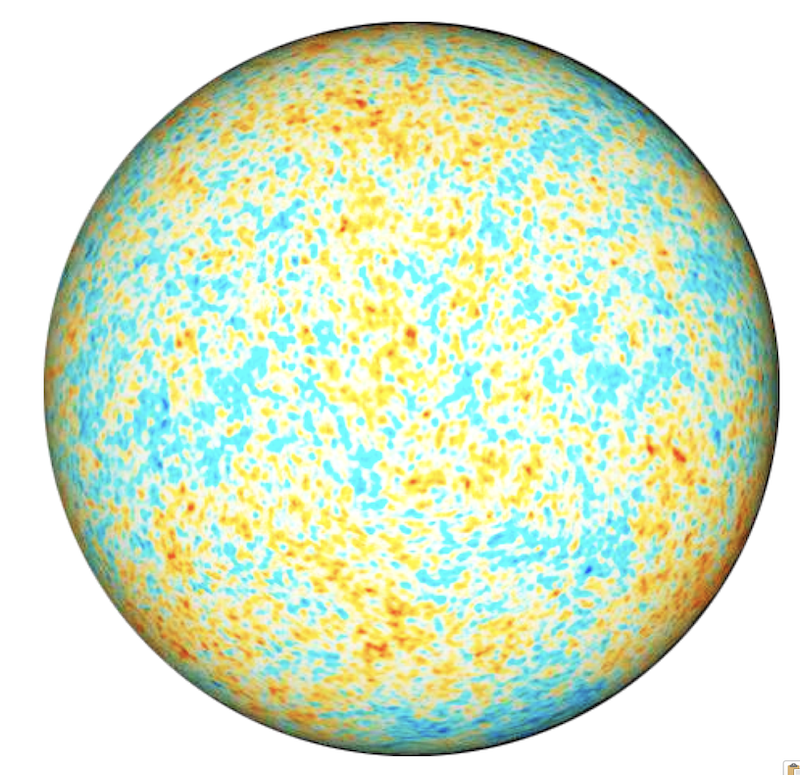
\includegraphics[width=0.9\linewidth]{figures/planck.png}
Cosmic microwave background radiation, captured by the Planck space observatory, is a signal on $\mathbb{S}^2$. 
}
the two-dimensional sphere $\Omega = \mathbb{S}^2$ with the group of rotations, the {\em special orthogonal group} $\fG = \mathrm{SO}(3)$.  
%
While chosen for pedagogical reason, this example is actually very practical and arises in numerous applications. In astrophysics, for example, observational data often naturally has spherical geometry. Furthermore, spherical symmetries are very important in applications in chemistry when modeling molecules and trying to predict their properties, e.g. for the purpose of virtual drug screening.
%\michael{ADD: molecules/astrophysics}


Representing a point on the sphere as a three-dimensional unit vector $\mathbf{u} : \|\mathbf{u}\|=1$, the action of the group can be represented as a $3\times 3$ orthogonal matrix $\mathbf{R}$ with $\mathrm{det}(\mathbf{R}) = 1$. The spherical convolution can thus be written as the inner product between the signal and the rotated filter,
$$
(x\star \theta)(\mathbf{R}) = \int_{\mathbb{S}^2} x(\textbf{u}) \theta(\mathbf{R}^{-1}\mathbf{u}) \mathrm{d}\mathbf{u}.
\marginnote{
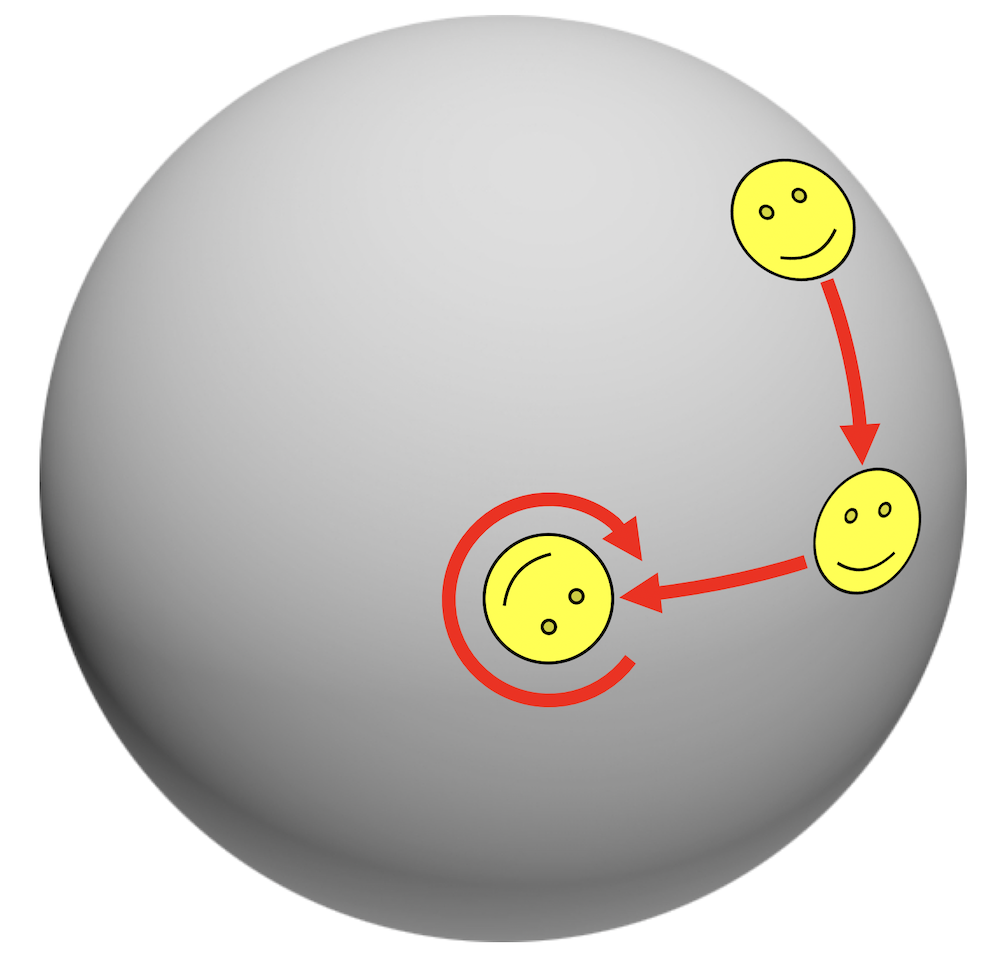
\includegraphics[width=0.9\linewidth]{figures/so3.png}
The action of $\mathrm{SO}(3)$ group on $\mathbb{S}^2$. Note that three types of rotation are possible; the $\mathrm{SO}(3)$ is a three-dimensional manifold.  
}
$$


The first thing to note is than now the group is not identical to the domain: the group $\mathrm{SO}(3)$ is a Lie group that is in fact a three-dimensional manifold, whereas $\mathbb{S}^2$ is a two-dimensional one.  
%
Consequently, in this case, unlike the previous example, the  convolution is a function {\em on} $\SO{3}$ {\em rather than on} $\Omega$. 

%\michael{\bf [ADD: a figure showing the difference between the sphere and SO(3) and why integration on S would give only isotropic filters.]}


This has important practical consequences: in our Geometric Deep Learning blueprint, we concatenate multiple equivariant maps (``layers'' in deep learning jargon) by applying a subsequent operator to the output of the previous one. 
%
In the case of translations, we can apply multiple convolutions in sequence, since their outputs are all defined on the same domain $\Omega$. 
%
In the general setting, since $x \star \theta$ is a function on $\fG$ rather than on $\Omega$, we cannot use exactly the same operation subsequently---it means that the next operation has to deal with {\em signals on $\fG$}, i.e. $x \in \mathcal{X}(\fG)$.  
%
Our definition of group convolution allows this case: 
we take as domain $\Omega = \fG$ acted on by $\fG$ itself via the group action $(\fg, \fh) \mapsto \fg \fh$ defined by the composition operation of $\fG$.
This yields the representation $\rho(\fg)$ acting on $x \in \mathcal{X}(\fG)$  by $(\rho(\fg) x)(\fh) = x(\fg^{-1}\fh)$\marginnote{The representation of $\fG$ acting on functions defined on $\fG$ itself is called the \emph{regular representation} of $\fG$.}.
% where $\fg, \fh$ and their composition $\fg^{-1}\fh$ belong to the group $\fG$.
Just like before, the inner product is defined by integrating the %product of $x$ and $\psi$ 
point-wise product of the signal and the filter 
over the domain, which now equals  $\Omega = \fG$.
%
In our example of spherical convolution, a second layer of convolution would thus have the form
$$
((x\star \theta)\star \phi)(\mathbf{R}) = \int_{\mathrm{SO}(3)} (x\star \theta)(\textbf{Q}) \phi(\mathbf{R}^{-1}\mathbf{Q}) \mathrm{d}\mathbf{Q}.
$$


%Now consider $\Omega = \R^2$ with  the group $\fG = \SE{2}$ of planar rotations and translations.\marginnote{$\SE{2}$ is called the {\em special Euclidean group} and is a subgroup of the Euclidean (isometry) group that additionally includes reflection. } 
%The first thing to note is that now the group elements (roto-translations) are not identical to the points on the domain. Consequently, in this case, unlike the previous example, the group convolution $x\star \psi$ given as the inner product between the signal and the transformed filter is a function {\em on} $\SE{2}$ {\em rather than on} $\Omega$. 

%\taco{TODO: Figure of SE2 group conv. Both planar to group, and group to group.}




%Our construction can be generalized to signals on any (locally compact) group $\fG$ and any $\Omega$ acted on by $\fG$ (in a sufficiently nice way).
%$\Omega$ is said to be a {\em homogeneous space} if for any two points $u, v \in \Omega$ one can be transformed into another, $u = \fg v$, by a symmetry $\fg \in \fG$. 
%that maps one to the other, .
%As noted before, for any such space $\Omega$, we have a regular representation $\rho(\fG)$ of $\fG$ acting on the space of signals $\mathcal{X}(\Omega)$. \michael{Bring the definition of homogeneous space earlier to Sec 1.2.1}
%
%As we will show in Chapter ???, for any two homogeneous spaces $\Omega$ and $\Omega'$ and a group $\fG$, one can define a convolution that maps between $\mathcal{X}(\Omega)$ and $\mathcal{X}(\Omega')$ in an equivariant manner, and indeed the most general linear equivariant map between these spaces is a convolution.

Since convolution involves inner product that in turn requires integrating over the domain $\Omega$, we can only use it on domains $\Omega$ that are small (in the discrete case) or low-dimensional (in the continuous case).  
% 
For instance, we can use convolutions on the plane $\R^2$ (two dimensional) or special orthogonal group $\SE{3}$ (three dimensional), or on the finite set of nodes of a graph ($n$-dimensional), but we cannot in practice perform convolution on the group of permutations $\Sigma_n$, which has $n!$ elements. 
%
Likewise, integrating over higher-dimensional groups like the affine group (containing  translations, rotations, shearing and scaling, for a total of $6$ dimensions) is not feasible in practice. 
%
Nevertheless, as we have seen in Section \ref{sec:gnn-intro}, we can still build equivariant convolutions for large groups $\fG$ by working with signals defined on low-dimensional spaces $\Omega$ on which $\fG$ acts.
Indeed, it is possible to show that any equivariant linear map $f : \mathcal{X}(\Omega) \rightarrow \mathcal{X}(\Omega')$ between two domains $\Omega, \Omega'$ can be written as a generalised convolution similar to the group convolution discussed here. %\michael{Taco: I don't understand what you want to say here.}

Second, we note that the Fourier transform we derived in the previous section from the shift-equivariance property of the convolution can also be extended to a more general case by projecting the signal onto the matrix elements of irreducible representations of the symmetry group. We will discuss this in future work. 
%
In the case of $\SO{3}$ studied here, this gives rise to the {\em spherical harmonics} and {\em Wigner D-functions}, which find wide applications in quantum mechanics and chemistry.


Finally, we point to the assumption that has so far underpinned our discussion in this section: whether $\Omega$ was a grid, plane, or the sphere, we could transform every point into any other point, intuitively meaning that all the points on the domain ``look the same.'' % by means of a rotation  
%
A domain $\Omega$ with such property is called a {\em homogeneous space}, where for any $u, v\in \Omega$ there exists $\mathfrak{g}\in\fG$ such that 
$
\mathfrak{g}.u = v\marginnote{The additional properties, $\mathfrak{e}.u = u$ and $\mathfrak{g} (\mathfrak{h}. u) = (\mathfrak{gh}). u$ are tacitly assumed here. }
$.
%
In the next section we will try to relax this assumption. 

%Consider as given a space $\Omega$, such as $\Omega = \R^2$, $\Omega = \Z^2$, or $\Omega = S^2$ (the sphere).
%Furthermore, let $G$ be a group of symmetries acting on $\Omega$, such as the group of roto-translations acting on $\R^2$, or the group or 3D rotations acting on the sphere.
%The inputs and feature maps of our generalized CNN are modelled as signals on $\Omega$, defined as $\mathcal{X}_\Omega = \{f : \Omega \rightarrow \R\}$\marginnote{In practice one would usually want to use multiple channels $c$, i.e. $f : \Omega \rightarrow \R^c$ but to reduce clutter we consider a single channel / grayscale image for now.}.
%From the action of $G$ on $\Omega$, we can derive an action of $G$ on $\mathcal{X}_\Omega$:
%\begin{equation}
%	\rho(g) f(x) = f(g^{-1} x)
%\end{equation}
%When $G$ is the translation group, this is just the \emph{shift operator} defined in the previous section.
%Similarly, when $G$ is the roto-translation group, this operator tells us how to roto-translate an image of filter $f$.

%In order to match a filter and an image / feature map, we define an inner product:
%\begin{equation}
%    \langle f, \psi \rangle = \int_{\Omega} f(x) \psi(x) d\mu(x),
%\end{equation}
%where $\mu$ is an invariant measure on $\Omega$. % too technical?
%In the case where $\mu$ is discrete, the inner product is a sum over the ``dimensions'' $x$ of the product of the vector components $f(x) \psi(x)$. 

%Having defined how to transform filters and match patterns, we are ready to define the generalized convolution:
%\begin{equation}
%    \label{eq:group-conv}
%    f \star \psi(g) = \langle f, \rho(g) \psi \rangle = \int_\Omega f(x) \psi(g^{-1} x) %d\mu(x).
%\end{equation}

%Let's look at some examples.
%When $\Omega = \Z_n = \{1, \ldots, n\}$ and $G = \Z_n$ (i.e. we consider signals on $\Z_n$ and the group of cyclic shifts) as in the last section, we retrieve the usual discrete convolution.
%To see this, note that $g^{-1} x$ in the equation above means: invert the group element $g \in G$ (in this example, the inverse of $g \in \Z_n$ is $-g$) and then act on $x \in \Omega$ (in this example, we get $x - g$.
%So the equation boils down to $f \star \psi(g) = \sum_i f(i) f(i - g)$.

%Now consider $\Omega = \R^2$ and $G = \SE{2}$, the group of rotations and translations acting on the plane.
%The first thing to note is that $f \star \psi$ is a function on $G = \SE{2}$ rather than a function on $\Omega$.
%In the previous example $\Omega = G$ so the distinction does not matter, but here it does.
%The group convolution computes the similarity between the input and filter for each transformation of the filter.



%Since the feature map $f \star \psi$ is a function on $G$ rather than $\Omega$, we cannot use exactly the same operation for the second and higher layers of the network.
%The solution is easy enough, though: for the second layer we define $\Omega_2 = G$, so that the feature space consists of functions $f : G \rightarrow \R$.
%We again define a shift operator $\rho_2(g)$ acting on such functions by $(\rho(g) f)(h) = f(g^{-1} h)$, where now $g^{-1} h$ refers to composition in the group $G$ (c.f. $g^{-1} x$ for $x \in \Omega$ refering to the group action of $G$ on $\Omega$).
%With these definitions, the exact same Equation \ref{eq:group-conv} defines the group convolution for second and higher layers.

%As a final example, consider spherical CNNs.
%Here we take the domain $\Omega_1 = S^2$ (the sphere) for the input space, and $G = \SO{3}$ the rotation group as symmetries.

%\taco{TODO: all of the above should be more conversational. Maybe focus on one example?}

%\michael{Generalised Fourier transform using representation theory. Bring up again the notion of multidimensional frequencies and show here where it comes from. }


%\michael{{\bf Say something along the lines:} 
%The important difference between the above examples and the case of sets and graphs is that on the grid, plane, or sphere we can represent our group with a small number of parameters: in case case of $\Z_n$, this is just one index, in the case of $\mathbb{R}^2$, this is translation vector and rotation angle, and in the case of the sphere ... 
%
%Conversely, on sets or graphs, the permutation group does not have such a low-dimensional representation and has a combinatorial complexity. 

%Show again why on graphs we don't have multi-dimensional Fourier transform. 
%}

%\michael{Talk about homogeneous vs non-homogenous spaces, using the example of graphs. Make it a segway to the next section}


%[Fourier theory]


\subsection{Geodesics and Manifolds}
\label{sec:geomanifoldsec}
%\michael{\bf [TACO: pls check if you are ok with this narrative. I start with homogeneous spaces, manifolds, then parallel transport. Then we can say that there is a broader view and talk about bundles in general]}

%\joan{
%Some high-level comments on what's written so far. 
%The generalization from groups to gauges is non-trivial, and I think it would be helpful to illustrate this extra level of generality with a running example. 
%In particular, an important innovation is that now we associate input data to certain vector fields on the domain; this is different from before. 
%It seems that this is the setting where the gauge equivariance is best motivated (unless I missed something), and I assume we can still use certain tasks from particle physics to motivate it.
%In other words, so far in our previous applications, the symmetry group acts on signals $\mathcal{X}(\Omega, \gV)$ only through $\Omega$, leaving the channels unchanged (just transporting them along the group action in $\Omega$). Now the situation is different and the gauge transformation is acting on the channels. 
%}

%\joan{I had a quick pass and the section reads very well; the build-up is coherent and objects are introduced keeping the intuition in mind (and adding figures to the margins will be even more helpful. 

%In particular, we can highlight that, contrary to the previous example of a fixed (curved) domain, many applications consider a variable geometric domain, and we wish to obtain signal representations that satisfy certain properties, namely (i) they are intrinsic, ie since the domain is defined only up to isometry, the signal representation should be invariant to isometries, and (ii) stability properties as this geometric domain changes. 
%These two aspects require introducing minimal elements of riemannian geometry 

%I have one comment/question though: currently we introduce the "minimal" elements of riemanian geometry that allow us to define convolutions and to describe the natural symmetries arising in manifold data (in particular isometry). 
%Would it be possible/convenient to highlight the invariance/stability priors early on, to motivate even further the need to introduce the different concepts (connection, parallel transport, isometries, geodesics, etc). In other words, the starting point is that we want to estimate a function $f$ defined over $\gX(\Omega, \R^s)$ that satisfies certain priors. The first and most natural prior is that $f$ is defined up to isometric transformations of $\Omega$. The second (if appropriate) is again the scale separation, ie local statistics in $x \in \gX(\Omega, \R^s)$ dominate. Then we explain how these priors lead again naturally to the GDL template by appropriately extending the notion of convolution. Additionally, it could be pertinent to describe how these priors relate to the stability of $f$ with respect to small changes in the metric structure of $\Omega$. 


%}


In our last example, the %domain $\Omega$ was the 
sphere $\mathbb{S}^2$ \marginnote{As well as the group of rotations $\mathrm{SO}(3)$, by virtue of it being a {\em Lie group}. }
was a {\em manifold}, albeit a special one 
%: every point $u$ on $\mathbb{S}^2$ can be rotated into any other point $v$, intuitively meaning that all the points on the sphere ``look the same.'' % by means of a rotation  
%
%A domain $\Omega$ with such property is called a {\em homogeneous space}, where for any $u, v\in \Omega$ there exists %$\frak{g}\in\fG$ such that 
%$
%\frak{g}.u = v\marginnote{The additional properties, %$\frak{e}.u = u$ and $\frak{g}.(\frak{h}.u) = (\frak{gh}).u$ %are tacitly assumed here. }
%$.
%%
%Homogeneous spaces thus have a 
with a global symmetry group due to its homogeneous structure. 
%
Unfortunately, this is not the case for the majority of manifolds, which typically do not have global symmetries. 
%
In this case, we cannot straightforwardly define an action of $\fG$ on the space of signals on $\Omega$ and use it to `slide' filters around in order to define a convolution as a direct generalisation of the classical construction. 
%. \joan{why would we want to translate signals in the manifold?}
%
Nevertheless, manifolds do have two types of invariance %symmetries
%various kinds of \emph{local} symmetries 
that we will explore in this section: transformations preserving metric structure and local reference frame change.  
%local \emph{gauge symmetries}, which we will now explore. 

While for many machine learning readers manifolds might appear as somewhat exotic objects, they are in fact very common in various scientific domains. In physics, manifolds play a central role as the model of our Universe --- according to Einstein's General Relativity Theory, gravity arises from the curvature of the space-time, modeled as a pseudo-Riemannian manifold.  
%
In more `prosaic' fields such as computer graphics and vision, manifolds are a common mathematical model of 3D shapes.\marginnote{The term `3D' is somewhat misleading and refers to the {\em embedding space}. The shapes themselves are 2D manifolds (surfaces).}  % 
%
The broad spectrum of applications of such models ranges from virtual and augmented reality and 
special effects obtained by means of `motion capture' to structural biology dealing with protein interactions that stick together (`bind' in chemical jargon) like pieces of 3D puzzle. 
%
The common denominator of these applications is the use of a manifold to represent the boundary surface of some 3D object. 


There are several reasons why such models are convenient.\marginnote{
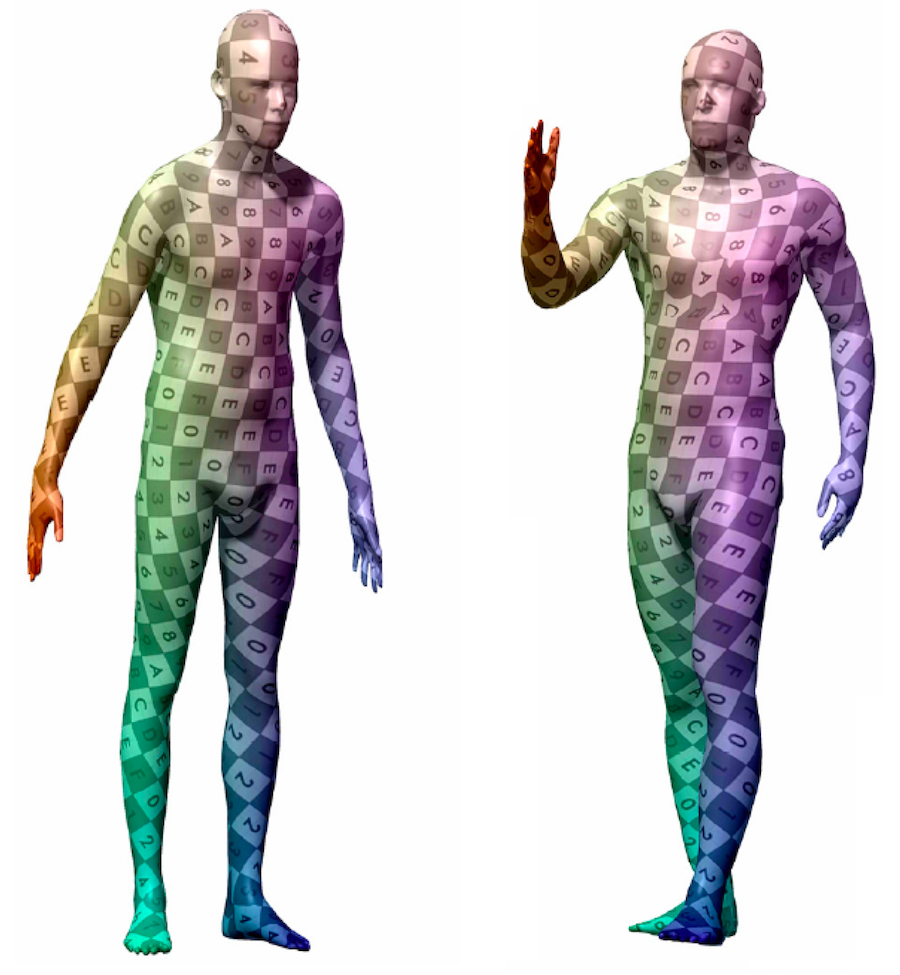
\includegraphics[width=0.9\linewidth]{figures/humans.png}
The human body is an example of a non-rigid object deforming in a  nearly-isometric way. 
} First, they offer a compact description of the 3D object, eliminating the need to allocate memory to `empty space' as is required in grid-based representations. 
%
Second, they allow to ignore the internal structure of the object. This is a handy property for example in structural biology where the internal folding of a protein molecule is often irrelevant for interactions that happen on the molecular surface. 
%
Third and most importantly, one often needs to deal with {\em deformable objects} that undergo non-rigid deformations. Our own body is one such example, and many applications in computer graphics and vision, such as the aforementioned motion capture and virtual avatars, require {\em deformation invariance}.
Such deformations can be modelled very well as transformations that preserve the intrinsic structure of a (Riemannian) manifold, namely the distances between points measured \emph{along} the manifold, without regard to the way the manifold is embedded in the ambient space.

%Here, we should emphasize that 
We should emphasise that %similarly to the case of graphs, 
manifolds fall under the setting of {\em varying domains} in our Geometric Deep Learning blueprint, and in this sense are similar to graphs. We will highlight the importance of the notion of invariance to domain deformations -- what we called `geometric stability' in Section~\ref{sec:geom_stab}. 
%
Since differential geometry is perhaps less familiar to the machine learning audience, we will introduce the basic concepts required for our discussion and refer the reader to \cite{penrose2005road} for their detailed exposition.  

%we have briefly mentioned before. 
%That is, unlike grid of homogeneous spaces we have discussed before where the domain can be assumed fixed and we are concerned with different signals on 

%\taco{Should we clarify why we need manifolds if we want deformation invariance? Also, should we call it deformation insensitivity? Since invariance would imply invariance to arbitrarily large deformations (just compose many small ones, each of which the net is invariant to.)}
%\michael{The proper term is isometry invariance. Isometry is understood in two senses: Riemannian (local metric=quadratic form on tangent space) and metric (geodesic distance). The two are equivalent on geodesically complete spaces due to Hopf-Rinow, which implies we can access the whole manifold through exp map from a single point. }

%\michael{STORY: we want to say that all models we build here are isometry-invariant, by virtue of being intrinsically constructed. This requires the definition of a Riemannian manifold. We can also refer to spectral techniques. 
%
%We then discuss gauges in this perspective, and then say that this is a much broader picture that does not need any metric, nor manifold, and can be defined on a bundle which is a topological construct. 
%}

%\joan{This is a good place to motivate geometric DL models that would fall beyond the homogeneous category: give a representative example that we can use throughout the rest of the section to guide the reader.} \michael{I think we focus this section on the domains, rather than on DL models. We should probably defer it to the discussion of Gauge CNNs.}


%\michael{Taco: why use $s$ and not $d$ for the manifold dimension? Do you want to decouple the feature dimension from the dimension of the manifold? } \joan{I switched from $d$ to $s$ since we used $d$ to refer to the dimensionality of the data and not the intrinsic dimension of the domain}
%
%\paragraph{Riemannian manifolds}
%\label{sec:manifolds}
%
%Since the formal definition of a manifold\marginnote{By `smooth' we mean differentiable suffient number of times, which is tacitly assumed for convenience. `Deformed' here means \emph{diffeomorphic}, i.e., we can map between the two neighbourhoods using a smooth and invertible map with smooth inverse. %, called a diffeomorphism. 
%%In this way, we can choose smooth coordinates for neighbourhoods of the manifold.
%} is somewhat involved, we 
%%defer its detailed discussion to Chapter ??? and 
%prefer to provide an intuitive picture at the expense of some precision. 
%%
%In this context, we can think of a (differentiable or smooth) manifold as a smooth multidimensional curved surface %(or higher dimensional space) 
%that is \emph{locally Euclidean} in the sense that any small neighbourhood around any point it can be deformed
%%\marginnote{`Deformed' here means \emph{homeomorphic to}, i.e. we can map between the neighbourhoods using a continuous and invertible map with continuous inverse. In fact, we will assume the manifold is smooth, in which case the map should be a diffeomorphism -- smooth and invertible with smooth inverse.}
%to a neighbourhood of $\R^s$; 
%%A crucial difference between a manifold\marginnote{We also tacitly assume the manifold to be smooth, i.e. having a $\mathcal{C}^\infty$-differentiable set of transition functions between local spaces.} and a Euclidean space is that a manifold is only {\em locally} Euclidean:  %
%%a small neighbourhood (open set) around each point $u \in \Omega$ is homeomorphic 
%%\marginnote{A {\em homeomorphism} is a continuous map with continuous inverse that preserves topological properties.}  to 
%%(topologically equivalent) to $\mathbb{R}^s$; 
%%
%%by a homeomorphism called a {\em chart}; 
%%the dimension $d$ is that of the manifold, which 
%in this case the manifold is said to be $s$-{\em dimensional}. 
%%
%%The composition of two charts (or more precisely, a chart and an inverse of a chart) allows to transition between the local 
%%
%%
%%Since the manifold is smooth, 
%This allows us to 
%locally approximate the manifold around point $u$ through the \emph{tangent space} $T_u\Omega$.  %and called the {\em tangent space}.
%The latter can be visualized by thinking of a prototypical two-dimensional manifold, the sphere, and attaching a plane to it at a point: with sufficient zoom, the spherical surface will seem planar. 
%% This analogy however should not be taken literally, as manifolds are abstract objects existing on their own without any geometric realization.  % Taco: this may be a bit confusing for newbies
%%
%\marginnote{Formally, the tangent bundle is the {\em disjoint union} $\displaystyle T\Omega = \bigsqcup_{u\in \Omega} T_u\Omega$.} The collection of all tangent spaces is called the {\em tangent bundle}, denoted $T\Omega$; we will dwell on the concept of bundles in more detail in Section~\ref{sec:gauges}. 
%%later and also in Chapter ???.
%
%
%
%A {\em tangent vector}, which we denote by $X\in T_u\Omega$, can be thought of as a local displacement from point $u$. 
%%In order to give it a sense of {\em direction}, 
%In order to measure the \emph{lengths} of tangent vectors and  \emph{angles} between them, %, and {\em volumes}, 
%%
%\marginnote{A bilinear function $g$ is said to be {\em positive-definite} if $g(X,X)>0$ for any non-zero vector $X\neq 0$. If $g$ is expressed as a matrix $\mathbf{G}$, it means $\mathbf{G} \succ 0$. The determinant $|\mathbf{G}|^{1/2}$ provides a local volume element, which does not depend on the choice of the basis. } 
%%
%we need to equip the tangent space with additional structure, expressed as a 
%positive-definite bilinear function
%$g_u: T_u\Omega \times T_u\Omega \rightarrow \mathbb{R}$ depending smoothly on $u$. Such a function is 
%called a {\em Riemannian metric}, in honour of Bernhardt Riemann who introduced the concept in 1856, and can be thought of as an inner product on the tangent space, $\langle X, Y \rangle_u = g_u(X,Y)$, which is an expression of the angle between any two tangent vectors $X, Y \in T_u\Omega$. 
%%
%The metric also induces a norm $\| X \|_u = g_u^{1/2}(X,X)$ allowing to locally measure lengths of vectors. 
%
%
%
%We must stress that tangent vectors 
%\marginnote{Unfortunately, too often vectors are identified with their coordinates. 
%%, which in our view constitutes a crime against humanity. 
%To emphasize this important difference, we use $X$ to denote a tangent vector and $\mathbf{x}$ to denote its coordinates. }
%are abstract geometric entities that exists in its own right and are {\em coordinate-free}. If we are to express a tangent vector $X$ numerically as an array of numbers, we can only represent it as a list of coordinates $\mathbf{x}=(x_1, \hdots, x_s)$ {\em relative to some local basis} $\{ X_1, \hdots X_s \} \subseteq T_u\Omega$.   
%%
%Similarly, the metric can be expressed as an $s\times s$ matrix $\mathbf{G}$ with elements $g_{ij} = g_u(X_i,X_j)$ w.r.t that basis. %; however, we stress that the definition of Riemannian metric does not rely on any particular choice of basis %all our definitions are coordinate-free and exist independently of any basis choice
%%(this will be the centrepiece of the following section). 
%
%%that allows to measure length, angle, and volume in the tangent space. 
%%
%
%
%
%%an {\em inner product}.
%%In differential geometry, an inner product on $T_u\Omega$ depending smoothly on $u$ is called a {\em Riemannian metric}, in honour of Bernhardt Riemann who introduced the concept in 1856. %
%%We will denote a Riemannian metric as a$g_u: T_u\Omega \times T_u\Omega \rightarrow \mathbb{R}$ that allows to measure length, angle, and volume in the tangent space. 
%%
%
%%
%%of a vector $$
%%
%%angle between two tangent vectors $x,y \in T_u\Omega$, (expressed %as $\cos^{-1}\left( \frac{\g_u(x,y)$) and a length of the 
%
%
%A manifold equipped with a metric is called a
%{\em Riemannian manifold} and properties that can be expressed entirely in terms of the metric are said to be {\em intrinsic}. %
%This is a crucial notion for our discussion, as according to our template, we will be seeking to construct functions acting on signals defined on $\Omega$ that are invariant to metric-preserving transformations called {\em isometries} that, roughly speaking, deform the manifold without affecting its local structure. If such functions can be expressed in terms of intrinsic quantities, they are automatically guaranteed to be isometry-invariant and thus unaffected by isometric deformations. 
%%
%These results can be further extended to dealing with approximate isometries; this is thus an instance of the geometric stability (domain deformation) discussed in our blueprint. 
%
%
%%\taco{Taco: here we should probably make clear that we are not talking about symmetries in the sense of automorphisms, i.e. maps $\Omega \rightarrow \Omega$ that preserve the metric, but about isomorphisms, i.e. maps $\Omega \rightarrow \Omega'$ that preserve the metric. Note that we do not yet discuss this in the template, but as discussed we should.} 
%
%%\michael{Approx isometry - geometric stability}
%
%While, as we noted, the definition of a Riemannian manifold does not require a
%geometric realization in any space, it turns out that any smooth Riemannian manifold can be realized as a subset of a Euclidean space of sufficiently high dimension (in which case it is said to be `embedded' in that space) by using the structure of the Euclidean space to induce a Riemannian
%metric.\marginnote{This result is known as the {\em Embedding Theorem}, due to John Forbes Nash, who became a household name after the Hollywood movie The Beautiful Mind. The paper folding art of origami is a manifestation of different isometric embeddings of the planar surface in $\mathbb{R}^3$. \vspace{4mm}
%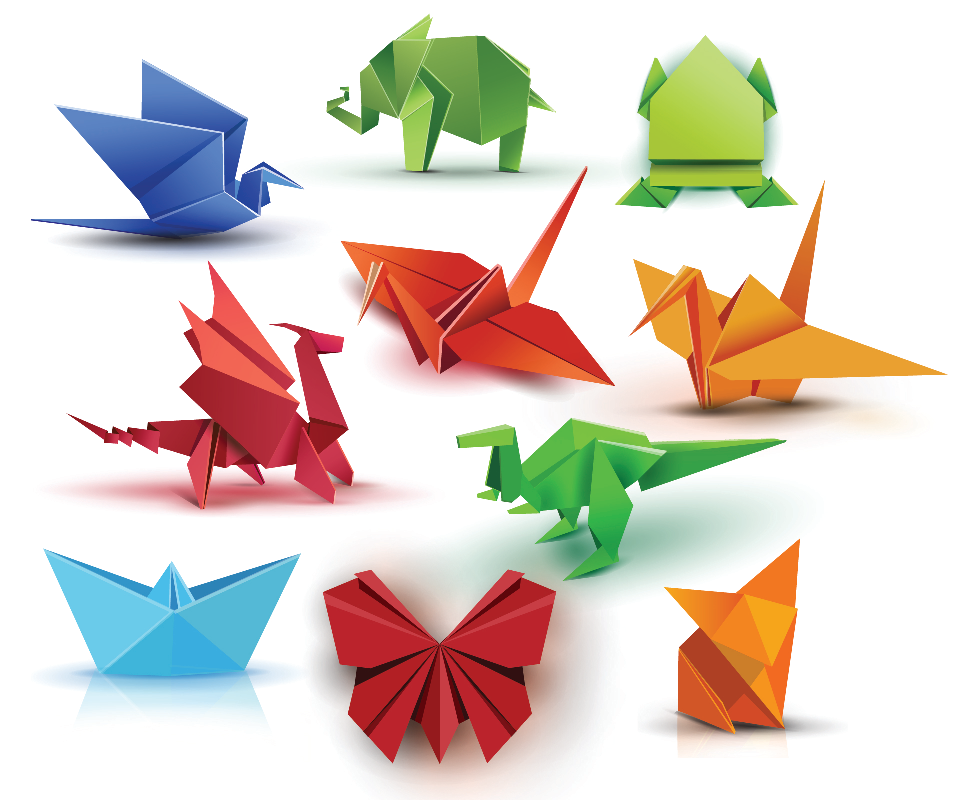
\includegraphics[width=1\linewidth]{figures/origami.pdf}
%}  Such an embedding is however not necessarily unique -- as we will see in the following, two different isometric 
%realizations of a Riemannian metric are possible. 
%%called {\em isometries}.
%
%
%
%
%
%\paragraph{Covariant derivative and Parallel transport}
%%
%Since we are interested in signals defined on $\Omega$, we need to provide the proper notion of scalar-
%%\marginnote{We will use the same notation for tangent and vector fields, the distinction between which will be clear from the context.} 
%and vector-valued functions on manifolds. 
%%
%A {\em scalar field} is a function of the form $x: \Omega\rightarrow \mathbb{R}$. 
%%
%%scalar-valued function  (often called a {\em scalar field}) $x: \Omega\rightarrow \mathbb{R}$ on the manifold. The space of 
%Scalar fields form a vector space $\mathcal{X}(\Omega, \mathbb{R})$ that can be equipped with the inner product %of scalar fields
%\begin{equation}
%\langle x, y \rangle = \int_\Omega x(u) y(u) \mathrm{d}u,
%\label{eq:inner_scalar}   
%\end{equation}
%%
%where $\mathrm{d}u$ % = \sqrt{\det g}$
%%\marginnote{More rigorously speaking, the volume form requires an inner product (i.e. Riemannian metric) and {\em orientation} (`handedness'). } 
%is the volume element induced by the Riemannian metric. 
%%
%%
%A (tangent) {\em vector field} is a function of the form $X: \Omega \rightarrow T\Omega$  assigning to each point a tangent vector in the respective tangent space, $u\mapsto X(u)\in T_u\Omega$.  
%%
%Vector fields also form a vector space $\mathcal{X}(\Omega, T\Omega)$ with the inner product defined through the Riemannian metric, 
%%
%\begin{equation}
%\langle X, Y \rangle = \int_\Omega g_u(X(u), Y(u)) \mathrm{d}u. \label{eq:inner_vector}   
%\end{equation}
%
%
%Another way to think of (and actually {\em define}) vector fields is as a generalised notion of derivative. 
%%
%In classical calculus, one can locally linearise a (smooth) function through the {\em differential} $\mathrm{d}x(u) = x(u+\mathrm{d}u) - x(u)$, which provides the change of the value of the function $x$ at point $u$ as a result of an inifinitesimal displacement $\mathrm{d}u$. 
%%
%However, in our case using this  definition na{\"i}vely brings up two problems: First, expressions of the form ``$u+\mathrm{d}u$'' are meaningless on manifolds, since there is no global vector space structure. 
%%, preventing us from adding or subtracting two points on $\Omega$. 
%%
%%
%A second problem arises when trying to take derivatives of vector fields, as one would need to subtract vectors belonging to tangent spaces at {\em different points}, while subtraction is only define \emph{within} a single vector space. 
%
%
%
%
%
%The solution to the first problem is to use tangent vectors as a model of local infinitesimal displacement. 
%%in order to provide a proper generalization of the differential on manifolds. 
%%
%Given a smooth scalar field $x\in \mathcal{X}(\Omega,\mathbb{R})$, we can think of a (smooth) vector field as a linear map $Y:\mathcal{X}(\Omega,\mathbb{R}) \rightarrow \mathcal{X}(\Omega,\mathbb{R})$ satisfying the properties of a {\em derivation}: 
%$Y(c) = 0$ for any constant $c$ (corresponding to the intuition that constant functions have vanishing derivatives), $Y(x+z) = Y(x) + Y(z)$ (linearity), and $Y(xz) = Y(x)z + xY(z)$ ({\em product} or {\em Leibniz rule}), for any smooth scalar fields $x,z \in \mathcal{X}(\Omega,\mathbb{R})$. 
%%
%It can be shown that one can use these properties to define vector fields axiomatically. 
%%
%The differential of $x$ can be defined as an operator $\mathrm{d}x : T\Omega \rightarrow \mathbb{R}$ of the form
%$$
%\mathrm{d}x(Y) = Y(x),
%$$
%which can be interpreted as follows: the change of $x$ as the result of displacement $Y \in T_u\Omega$ at point $u$ is given by $\mathrm{d}x(Y)$. 
%%
%It is thus an extension of the classical notion of {\em directional derivative}. 
%%
%Importantly, this construction {\em does not use the Riemannian metric whatsoever} and can thus be generalised to a broader construction of bundles discussed in the next section. 
%
%
%
%At each point $u$, the differential operator $\mathrm{d}x_u$ can be regarded as a {\em linear functional} acting on tangent vectors $X \in T_u\Omega$. Linear functionals on a vector space are called {\em dual vectors} or {\em covectors}; if in addition we are given an inner product (Riemannian metric), a dual vector can always be represented as 
%\marginnote{This is a consequence of the Riesz-Fr{\'e}chet Representation Theorem, by which every dual vector can be expressed as an inner product with a vector. } 
%$$
%\mathrm{d}x_u (X)  = g_u(\nabla x(u), X).
%$$ 
%The representation of the differential at point $u$ is a tangent vector $\nabla x(u) \in T_u \Omega$ called the (intrinsic) {\em gradient} of $x$; similarly to the gradient in classical calculus, it can be thought of as the direction of the steepest increase of $x$. 
%%
%%More generally, the gradient can be thought of as an operator $\nabla : $
%
%
%
%
%In a similar way, we can axiomatically define the {\em covariant derivative} $\nabla_Y X$ of a smooth vector field $X$ along another smooth vector field $Y$ as an operator  
%$\nabla : T\Omega \times T\Omega \rightarrow T\Omega$ %associating the vector fields $(X,Y) \mapsto \nabla_Y X$ and satisfying the following properties: 
%of the following form:
%
%
%\begin{tcolorbox}[width=\linewidth,
%              boxsep=0pt,
%              left=7.5pt,
%              right=7.5pt,
%              top=7.5pt,
%              bottom=7.5pt,
%              arc=0pt,
%              boxrule=0pt,toprule=0pt,
%              colback=boxgray,
%              ]%%
%A  {\em covariant derivative} (or {\em connection}) is a map $(X,Y) \mapsto \nabla_Y X$
%satisfying, 
%for all smooth scalar fields $x, y \in \mathcal{X}(\Omega, \mathbb{R})$ and smooth vector fields $X, Y, Z \in \mathcal{X}(\Omega, T\Omega)$, 
%the following axioms: \vspace{3mm}\\
%%\begin{enumerate}
%%\item 
%\noindent {\em Linearity (w.r.t. first argument):} 
%$\nabla_{xY + yZ}(X) = \nabla_Y(X)x + \nabla_Z(X)y$.\vspace{2mm}\\
%\noindent  {\em Additivity (w.r.t. second argument):}
%%\marginnote{For an {\em affine connection}, the additivity requirement is dropped. } 
%$\nabla_Y(X+Z) = \nabla_Y X + \nabla_Y Z$.\vspace{2mm}\\
%\noindent  {\em Product rule:} $\nabla_Y(zX) = z \nabla_Y(X) + \mathrm{d}z(Y) X$, where for scalar fields the covariant derivative coincides with the differential,  
%%, where in the second term  
%$\nabla_Y(z) = \mathrm{d}z(Y)$.%\vspace{2mm}
%%
%%    \noindent  
%%\end{enumerate}
%
%\end{tcolorbox}
%
%Covariant derivative allows {\em parallel transport}, or a way of moving tangent vectors along a curve so they are ``pointing in the same direction''.  
%%
%Given a smooth curve $\gamma : [0,T] \rightarrow \Omega$, a vector $X$ is said to be parallel transported along $\gamma$ if $\nabla_{\gamma'(t)} X(\gamma(t)) = 0$ for $t \in [0,T]$, where $\gamma'(t) \in T_{\gamma(t)} \Omega$ is the tangent to the curve. 
%%
%Intuitively, this implies that the vector remains `constant'\marginnote{
%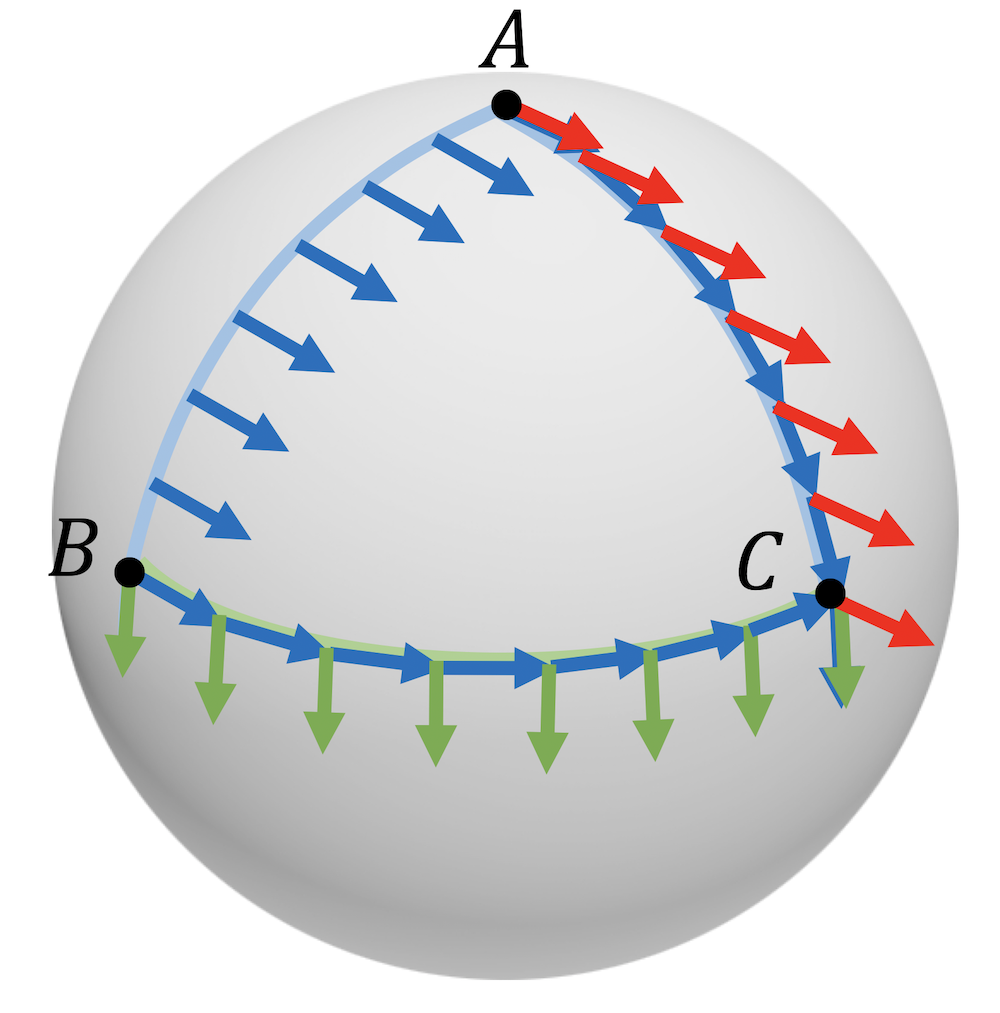
\includegraphics[width=0.9\linewidth]{figures/parallel.png}
%Euclidean transport of a vector from A to C makes no sense on the sphere, as the resulting vectors (red) are not in the tangent plane. Parallel transport from A to C (blue) rotates the vector along the path. It is path dependent: going along the path BC and ABC produces different results.  
%} (the derivative vanishes) for a small displacement along the curve. 
%%
%The result of the transport is path-dependent, which is best visualised on the sphere (see insert): moving a vector from the north pole to the equator along two different curves produces different results.
%%
%The name `connection' stems from the fact that parallel transport defines a linear isomorphism between tangent spaces along the curve $\gamma$, that is, a way to transport vectors from $T_{\gamma(0)}\Omega$ to $T_{\gamma(T)}\Omega$, thereby `connecting' these spaces.
%
%
%%which transports its tangent along itself 
%
%
%%perform  
%%of tangent vectors by (in this way, it ``connects'' two tangent spaces at different points, hence the alternative name `connection').  
%
%It is important to note that the definition of the covariant derivative  %and geodesic 
%does not rely on the metric, and  
%in fact, is an abstract construction that extends beyond Riemannian manifolds. %there are multiple ways to define one.  
%%
%When one is given a Riemannian metric, of particular interest is a special kind of covariant derivative called the {\em Levi-Civita connection}, after the Italian mathematician Tullio Levi-Civita who introduced the notion in 1917. %\marginnote{}
%%
%
%
%\begin{tcolorbox}[width=\linewidth,
%              boxsep=0pt,
%              left=7.5pt,
%              right=7.5pt,
%              top=7.5pt,
%              bottom=7.5pt,
%              arc=0pt,
%              boxrule=0pt,toprule=0pt,
%              colback=boxgray,
%              ]%%
%The {\em Levi-Civita connection} on a Riemannian manifold with metric $g$ is a connection $\nabla$ that additionally satisfies the following properties:
%\vspace{3mm}\\
%%\begin{enumerate}
%%\item 
%    \noindent  {\em Torsion free:} \marginnote{Roughly, {\em torsion} describes how tangent vectors twist about the curve when parallel transported, and {\em curvature} how they roll along it. }
%$\nabla_X Y - \nabla_Y X = [X,Y]$, where the tangent vector field $[X,Y] \in \mathcal{X}(\Omega, T\Omega)$ is the 
%{\em commutator} (also known as the {\em Lie bracket} or {\em Lie derivative}), defined by its action on scalar fields 
%$$[X,Y](z) = X(Y(z)) - Y(X(z)).$$
%%\vspace{2mm}\\
%%    
%\noindent {\em Preserves the metric:}\marginnote{Connection with this property is also known as {\em metric} or {\em metric-compatible}.} 
%$\nabla g = 0$, which is understood as 
%$$
%(\nabla_X g)(Y,Z) = X(g(Y,Z)) - g(\nabla_X Y, Z) - g(Y, \nabla_X Z) = 0.
%$$
%for any smooth $X, Y$, and $Z$. 
%
%\end{tcolorbox}
%
%
%%
%%
%The condition $\nabla g = 0$ (metric compability) implies that the metric remains invariant under parallel transport, i.e., parallel transport preserves the length of the tangent vectors (and is thus an isometry). 
%%
%The torsion-free properties make the Levi-Civita connection {\em unique}, a result known as the Fundamental Theorem of Riemannian Geometry. 
%%
%%\marginnote{
%For this reason, in Riemannian geometry the term `connection' is usually synonymous with the Levi-Civita connection, which can be considered a `canonical' connection.
%
%%guaranteeing that every Riemannian manifold admits a unique Levi-Civita connection, making it thus the `canonical' one. 
%
%
%
%
%%\taco{I think the notion of Torsion will be difficult to understand for newbies. Also, we are differentiating a tensor field g which I think we have not explained yet.
%
%%We could consider just mentioning the LC connection and explaining that parallel transport defined wrt it will not change the length of tangent vectors. We can also say that if another condition (Torsion free) is satisfied, there is a unique LC connection, without formalizing it.}
%
%
%
%\paragraph{Geodesics and Exponential map}
%
%A curve $\gamma$ along which parallel transport preserves the tangent vector to the curve,\marginnote{From the Greek \textgreek{geodai\textsigma{}{\'i}a}, literally `division of Earth'.}  i.e., $\nabla_{\gamma'} \gamma' = 0$ is called {\em geodesic}.
%%
%Locally at a point $u$, it is always possible to define a unique geodesic in a given direction $X$, i.e. a smooth curve $\gamma_X : [0,T] \rightarrow \Omega$ satisfying $\gamma(0) = u$ and $\gamma'(0) = X$, for some small $T>0$. 
%%
%%
%This\marginnote{Here, $B_r(0)$ is a ball of radius $r$ around the origin. Note that geodesic completeness does not necessarily guarantee that $\exp$ is a diffeomorphism -- the largest radius $r$ about $u$ for which $\exp_u(B_r(0) \subseteq T_u\Omega)$ is mapped diffeomorphically is called the {\em injectivity radius}. } gives a natural mapping from (a subset of) the tangent space $T_u \Omega$ to $\Omega$ called the {\em exponential map} $\exp : B_r(0) \subset T_u\Omega \rightarrow \Omega$, which is defined by taking a unit step along the geodesic in the direction $X$, i.e., $\exp_u(X) = \gamma_X(1)$. %
%%
%%
%When $\gamma_X(t)$ is defined for all $t\geq 0$ (that is, we can shoot the geodesic from a point $u$ for as long as we like), the manifold is said to be {\em geodesically complete} and the exponential map is defined on the whole tangent space.
%%
%Since compact manifolds are geodesically complete, we can tacitly assume this convenient property. 
%
%
%
%%
%On Riemannian\marginnote{It is tacitly assumed that curves are given in {\em arclength parametrisation}, such that $\| \gamma' \| = 1$ (constant velocity).} manifolds with the Levi-Civita connection, one can show geodesics to be {\em length-minimising curve}, 
%%
%i.e., a geodesic $\gamma$ minimises the length functional 
%%
%$$
%L(\gamma) = \int_{0}^T \| \gamma'(t) \| \mathrm{d}t =  \int_{0}^T g_u^{1/2} (\gamma'(t), \gamma'(t)) \mathrm{d}t 
%$$
%%
%among all curves with endpoints $u = \gamma(0)$ and $v=\gamma(T)$. 
%%
%%
%Readers familiar with metric geometry are probably more used to this definition of geodesics as shortests paths. 
%%
%In fact, \marginnote{Hopf-Rinow Theorem thus estabilishes the equivalence between geodesic and metric completeness, the latter meaning every Cauchy sequence converges.} a result known as the Hopf-Rinow Theorem guarantees that geodesically complete manifolds are also {\em complete metric spaces}, in which one can realise a metric (called the {\em geodesic distance})  between any pair of points $u,v$ as the length of the shortest path between them
%$$
%d_g(u,v) = \min_{\gamma} L(\gamma) \quad\quad \text{s.t.} \quad\quad \gamma(0) = u, \,\, \gamma(T) = v,
%$$
%which exists (i.e., the minimum is attained).\marginnote{To avoid confusion with the Riemannian metric, we will use the term `distance'. Our notation $d_g$ makes the distance depend on the Riemannian metric, though the definition of $L$. }
%%
%Importantly, geodesic distances are intrinsic, being dependent solely on the Riemannian metric. 
%
%
%%The term `geodesic' is also used in metric geometry, where it is defined as the shortest path. In the setting described here the two meanings coincide. }
%
%
%%i.e., the two notions of `geodesic' used somewhat differently in differential and metric geometry
%
%
%
%
%
%%===
%%
%%
%%For a smooth scalar field\marginnote{Linear functionals acting on vectors are called {\em dual vectors} or {\em covectors}. By the Riesz-Fr{\'e}chet Representation Theorem, every covector can be expressed as an inner product with a vector. } $x: \Omega \rightarrow \mathbb{R}$, the differential can be thought of as an operator $dx : T\Omega \rightarrow \mathbb{R}$ acting on tangent fields. At each point, the differential can be expressed as a linear functional acting on tangent vectors
%%$dx(u)  = g_u(\nabla x(u), \cdot)$. 
%%%
%%%
%%Given a smooth vector field $Y$, 
%%the {\em covariant derivative} $\nabla_Y x$ of $x$ {\em along} $Y$ is defined as 
%%$(\nabla_Y x)(u) = g_u(\nabla x(u), Y(u))$
%%and is a generalisation of the corresponding notion in classical calculus. 
%%%
%%%The change of the value of $x$ as the result of 
%%%displacement $y \in T_u\Omega$ at point $u$ is thus given by applying the form to the tangent
%%%vector, $dx(u) y = g_u(\nabla x(u), y)$, and can be thought
%%%of as an extension of the notion of the classical directional
%%%derivative.
%%%
%%The vector field $\nabla x$ is called the (intrinsic) {\em gradient} of $x$; at each point, it indicates the direction of the steepest increase of $x$. 
%%%
%%%The symbol $\nabla$ can be though of as an operator acting on scalar fields and producing vector fields defined above.  
%%
%%
%%Given two smooth vector fields $x$ and $y$, the covariant derivative $\nabla_y x$ of $x$ along $y$
%%
%%
%%
%%
%%Connection is defined as an abstract map $\nabla : T\Omega \times T\Omega \rightarrow T\Omega$ associating $(x,y) \mapsto \nabla_y x$ in a way that is linear w.r.t. both $x$ and $y$ and also satisfies the {\em product rule} $\nabla_y(xz) = x\nabla_y z + z \nabla_y x$ for any vector fields $x,y$ and scalar field $z$. 
%%
%%
%%
%%When the manifold is embedded in a Euclidean space, the covariant derivative coincides with the standard Euclidean directional derivarive projected onto the tangent space. 
%%
%%
%%
%%
%%
%%
%%%known as the {\em pushforward} $d\eta : T\Omega \rightarrow T\Omega'$.  
%%
%%
%%
%%the notion of derivative describes how the value of a function changes with an infinitesimal change of its
%%argument. 
%%
%%
%%One of the big differences distinguishing classical
%%calculus from differential geometry is a lack of vector space
%%
%%
%%structure on the manifold, prohibiting us from na\"{i}vely using
%%expressions like $f(x+dx)$. The conceptual leap that is required
%%to generalize such notions to manifolds is the need to work
%%locally in the tangent space
%%
%%
%%
%%
%%
%%
%%
%%
%%
%%
%
%
%
%
%
%\paragraph{Isometries}
%Consider now a deformation of our manifold $\Omega$ into another manifold $\Omega'$ with a Riemannian metric $h$.
%%
%We will assume this map to be a diffeomorphism $\eta: (\Omega, g) \rightarrow (\Omega', h)$ between manifolds.   
%%
%Its differential $\mathrm{d}\eta : T\Omega \rightarrow T\Omega'$ defines a map between the respective tangent bundles (referred to as {\em pushforward}), such that   
%%\marginnote{The pushforward is what is called a {\em bundle map}.}
%at a point $u$, we have $\mathrm{d}\eta_u : T_u \Omega \rightarrow T_{\eta(u)}\Omega'$, %which allows to interpret it as follows: 
%%
%interpreted as before: 
%if we make a small displacement from point $u$ by tangent vector $X \in T_u \Omega$, the map $\eta$ will be displaced from point $\eta(u)$ by tangent vector $\mathrm{d}\eta_u(X) \in T_{\eta(u)}\Omega'$. 
%
%
%Since the pushforward provides a mechanism to associate tangent vectors on the two manifolds, it allows to {\em pullback }\marginnote{Pushforward and pullback are adjoint operators $\langle \eta^* \alpha, X \rangle = \langle \alpha, \eta_*X \rangle$ where $\alpha \in T^*\Omega$ is a {\em dual vector field}, defined at each point as a linear functional acting on $T_u\Omega$ and the inner products are defined respectively on vector and dual vector fields. } the metric $h$ from $\Omega'$ to $\Omega$, 
%$$
%(\eta^*h)_u(X,Y) = h_{\eta(u)}(\mathrm{d}\eta_u(X), \mathrm{d}\eta_u(Y))
%$$ 
%%
%If the pullback metric coincides at every point with that of $\Omega$, i.e., $g = \eta^*h$, the map $\eta$ is called  (a Riemannian) {\em isometry}. % (metric-preserving). 
%%
%For two-dimensional manifolds (surfaces), isometries can be intuitively understood as inelastic deformations that deform the manifold without `stretching' or `tearing' it. 
%
%
%
%By virtue of their definition, isometries preserve intrinsic structures such as geodesic distances, which are expressed entirely in terms of the Riemannian metric. % and Gaussian curvature.
%%
%Therefore, we can also understand isometries from the position of metric geometry,\marginnote{The Myers–Steenrod Theorem establishes that the converse is also true on connected manifolds: every metric isometry is also a Riemannian isometry. } 
%as distance-preserving maps {\em between metric spaces} $\eta : (\Omega, d_g) \rightarrow (\Omega', d_h)$, in the sense that 
%$$
%d_g (u,v) = d_h(\eta(u),\eta(v)) 
%$$
%for all $u,v \in \Omega$, 
%or more compactly, $d_g = d_h \circ (\eta \times \eta)$. 
%%where $d_g, d_g$ are the geodesic distances induced by the respective Riemannian metrics $g, h$. 
%%
%
%%[Gauss Theorema Egregium, definition of curvature through perimeter defect, pizza example]
%
%
%A particular case of the above is a diffeomorphism  of the domain itself, which we will denote by $\tau \in \mathrm{Diff}(\Omega)$. We will call it a Riemannian  \mbox{(self-)isometry} if the pullback metric satisfies $\tau^* g = g$, or a metric (self-)isometry if $d_g = d_g\circ (\tau \times \tau)$.
%%
%Not surprisingly, isometries form a group with the composition operator denoted by $\mathrm{Iso}(\Omega)$ and called the {\em isometry group}; the identity element is the map $\tau(u) = u$ and the inverse always exists (by definition of $\tau$ as a diffeomorphism). 
%%
%Self-isometries are thus {\em intrinsic symmetries} of manifolds.
%
%
%%Continuous symmetries on manifolds are infinitesimally generated
%%%\marginnote{More correctly, Killing fields are the infinitesimal generators of continuous symmetries. } 
%%by special tangent vector fields called {\em Killing fields}, named after Wilhelm Killing. A field $X$ is Killing if the  Lie derivative\marginnote{The Lie derivative in this case is a derivative of forms. For scalar and vector fields, it coincides with the covariant derivative $\mathcal{L}_X y = \nabla_X y$ and the commutator $\mathcal{L}_X Y = [X,Y]$, respectively. } of the Riemannian metric along it vanishes, $\mathcal{L}_X g = 0$, which is interpreted as 
%%%
%%$$
%%\mathcal{L}_X g(Y,Z) = g(\nabla_Y X, Z) + g(Y,\nabla_Z X) = 0
%%$$
%%for any smooth tangent fields $Y, Z$. 
%%%
%%We can recap that like we mentioned in Section~\ref{sec:symmetries}, we can regard symmetries as automorphisms (self-maps) preserving additional structure: either the local Riemannian metric, or global geodesic distances between pairs of points. 
%%%\taco{Do we need Killing fields? It's interesting but I worry that we'd need to properly introduce Lie derivatives to make it understandable.} \michael{Lets keep them for now}
%%%OK :)
%



\paragraph{Riemannian manifolds}
\label{sec:manifolds}

Since the formal definition of a manifold\marginnote{By `smooth' we mean differentiable suffient number of times, which is tacitly assumed for convenience. `Deformed' here means \emph{diffeomorphic}, i.e., we can map between the two neighbourhoods using a smooth and invertible map with smooth inverse. %, called a diffeomorphism. 
%In this way, we can choose smooth coordinates for neighbourhoods of the manifold.
} is somewhat involved, we 
%defer its detailed discussion to Chapter ??? and 
prefer to provide an intuitive picture at the expense of some precision. 
%
In this context, we can think of a (differentiable or smooth) manifold as a smooth multidimensional curved surface %(or higher dimensional space) 
that is \emph{locally Euclidean}, in the sense that any small neighbourhood around any point it can be deformed
%\marginnote{`Deformed' here means \emph{homeomorphic to}, i.e. we can map between the neighbourhoods using a continuous and invertible map with continuous inverse. In fact, we will assume the manifold is smooth, in which case the map should be a diffeomorphism -- smooth and invertible with smooth inverse.}
to a neighbourhood of $\R^s$; 
%A crucial difference between a manifold\marginnote{We also tacitly assume the manifold to be smooth, i.e. having a $\mathcal{C}^\infty$-differentiable set of transition functions between local spaces.} and a Euclidean space is that a manifold is only {\em locally} Euclidean:  %
%a small neighbourhood (open set) around each point $u \in \Omega$ is homeomorphic 
%\marginnote{A {\em homeomorphism} is a continuous map with continuous inverse that preserves topological properties.}  to 
%(topologically equivalent) to $\mathbb{R}^s$; 
%
%by a homeomorphism called a {\em chart}; 
%the dimension $d$ is that of the manifold, which 
in this case the manifold is said to be $s$-{\em dimensional}. 
%
%The composition of two charts (or more precisely, a chart and an inverse of a chart) allows to transition between the local 
%
%
%Since the manifold is smooth, 
This allows us to 
locally approximate the manifold around point $u$ through the \emph{tangent space} $T_u\Omega$.  %and called the {\em tangent space}.
The latter can be visualised by thinking of a prototypical two-dimensional manifold, the sphere, and attaching a plane to it at a point: with sufficient zoom, the spherical surface will seem planar (Figure~\ref{fig:sphere_metric}). 
% This analogy however should not be taken literally, as manifolds are abstract objects existing on their own without any geometric realization.  % Taco: this may be a bit confusing for newbies
%
\marginnote{Formally, the tangent bundle is the {\em disjoint union} $\displaystyle T\Omega = \bigsqcup_{u\in \Omega} T_u\Omega$.} The collection of all tangent spaces is called the {\em tangent bundle}, denoted $T\Omega$; we will dwell on the concept of bundles in more detail in Section~\ref{sec:gauges}. 
%later and also in Chapter ???.



A {\em tangent vector}, which we denote by $X\in T_u\Omega$, can be thought of as a local displacement from point $u$. 
%In order to give it a sense of {\em direction}, 
In order to measure the \emph{lengths} of tangent vectors and  \emph{angles} between them, %, and {\em volumes}, 
%
\marginnote{A bilinear function $g$ is said to be {\em positive-definite} if $g(X,X)>0$ for any non-zero vector $X\neq 0$. If $g$ is expressed as a matrix $\mathbf{G}$, it means $\mathbf{G} \succ 0$. The determinant $|\mathbf{G}|^{1/2}$ provides a local volume element, which does not depend on the choice of the basis. } 
%
we need to equip the tangent space with additional structure, expressed as a 
positive-definite bilinear function
$g_u: T_u\Omega \times T_u\Omega \rightarrow \mathbb{R}$ depending smoothly on $u$. Such a function is 
called a {\em Riemannian metric}, in honour of Bernhardt Riemann who introduced the concept in 1856, and can be thought of as an inner product on the tangent space, $\langle X, Y \rangle_u = g_u(X,Y)$, which is an expression of the angle between any two tangent vectors $X, Y \in T_u\Omega$. 
%
The metric also induces a norm $\| X \|_u = g_u^{1/2}(X,X)$ allowing to locally measure lengths of vectors. 



We must stress that tangent vectors 
are abstract geometric entities that exists in their own right and are {\em coordinate-free}. If we are to express a tangent vector $X$ numerically as an array of numbers, we can only represent it as a list of coordinates $\mathbf{x}=(x_1, \hdots, x_s)$ {\em relative to some local basis}\marginnote{Unfortunately, too often vectors are identified with their coordinates. 
%, which in our view constitutes a crime against humanity. 
To emphasise this important difference, we use $X$ to denote a tangent vector and $\mathbf{x}$ to denote its coordinates. } $\{ X_1, \hdots X_s \} \subseteq T_u\Omega$.   
%
Similarly, the metric can be expressed as an $s\times s$ matrix $\mathbf{G}$ with elements $g_{ij} = g_u(X_i,X_j)$ in that basis. 
%
We will return to this point in Section~\ref{sec:gauges}. 
%; however, we stress that the definition of Riemannian metric does not rely on any particular choice of basis %all our definitions are coordinate-free and exist independently of any basis choice
%(this will be the centrepiece of the following section). 

%that allows to measure length, angle, and volume in the tangent space. 
%

%\michael{Add a simple example here}


\begin{figure}[h!]
    \centering
    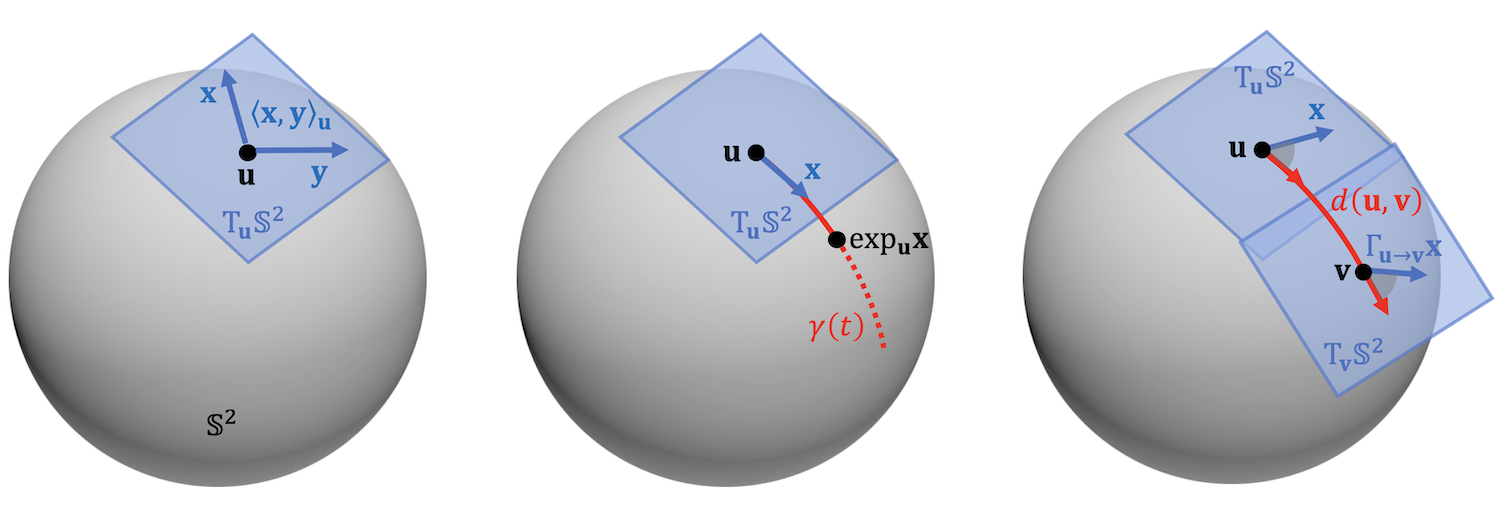
\includegraphics[width=\linewidth]{figures/manifold.png}
    \caption{
    Basic notions of Riemannian geometry illustrated on the example of the two-dimensional sphere $\mathbb{S}^2 = \{\mathbf{u}\in \mathbb{R}^3 : \|\mathbf{u}\|=1 \}$, realised a subset (sub-manifold) of $\mathbb{R}^3$. 
%
The tangent space to the sphere is given as $T_\mathbf{u}\mathbb{S}^2 = \{ \mathbf{x}\in \mathbb{R}^3 : \mathbf{x}^\top \mathbf{u} = 0\}$ and is a 2D plane -- hence this is a 2-dimensional manifold. The Riemannian metric is simply the Euclidean inner product restricted to the tangent plane, $\langle \mathbf{x}, \mathbf{y}\rangle_\mathbf{u} = \mathbf{x}^\top \mathbf{y}$ for any $\mathbf{x},\mathbf{x}\in T_\mathbf{u}\mathbb{S}^2$. 
The exponential map is given by 
$\exp_\mathbf{u}(\mathbf{x}) = \cos(\| \mathbf{x}\|)\mathbf{u} + \frac{\sin(\| \mathbf{x}\|)}{\|\mathbf{x}\|} \mathbf{x}$, for $\mathbf{x} \in T_\mathbf{u}\mathbb{S}^2$. 
%
Geodesics are great arcs of length $d(\mathbf{u},\mathbf{v}) = \cos^{-1}(\mathbf{u}^\top \mathbf{v})$.
    }
    \label{fig:sphere_metric}
\end{figure}%


%an {\em inner product}.
%In differential geometry, an inner product on $T_u\Omega$ depending smoothly on $u$ is called a {\em Riemannian metric}, in honour of Bernhardt Riemann who introduced the concept in 1856. %
%We will denote a Riemannian metric as a$g_u: T_u\Omega \times T_u\Omega \rightarrow \mathbb{R}$ that allows to measure length, angle, and volume in the tangent space. 
%

%
%of a vector $$
%
%angle between two tangent vectors $x,y \in T_u\Omega$, (expressed %as $\cos^{-1}\left( \frac{\g_u(x,y)$) and a length of the 


A manifold equipped with a metric is called a
{\em Riemannian manifold} and properties that can be expressed entirely in terms of the metric are said to be {\em intrinsic}. %
This is a crucial notion for our discussion, as according to our template, we will be seeking to construct functions acting on signals defined on $\Omega$ that are invariant to metric-preserving transformations called {\em isometries} that deform the manifold without affecting its local structure.\marginnote{
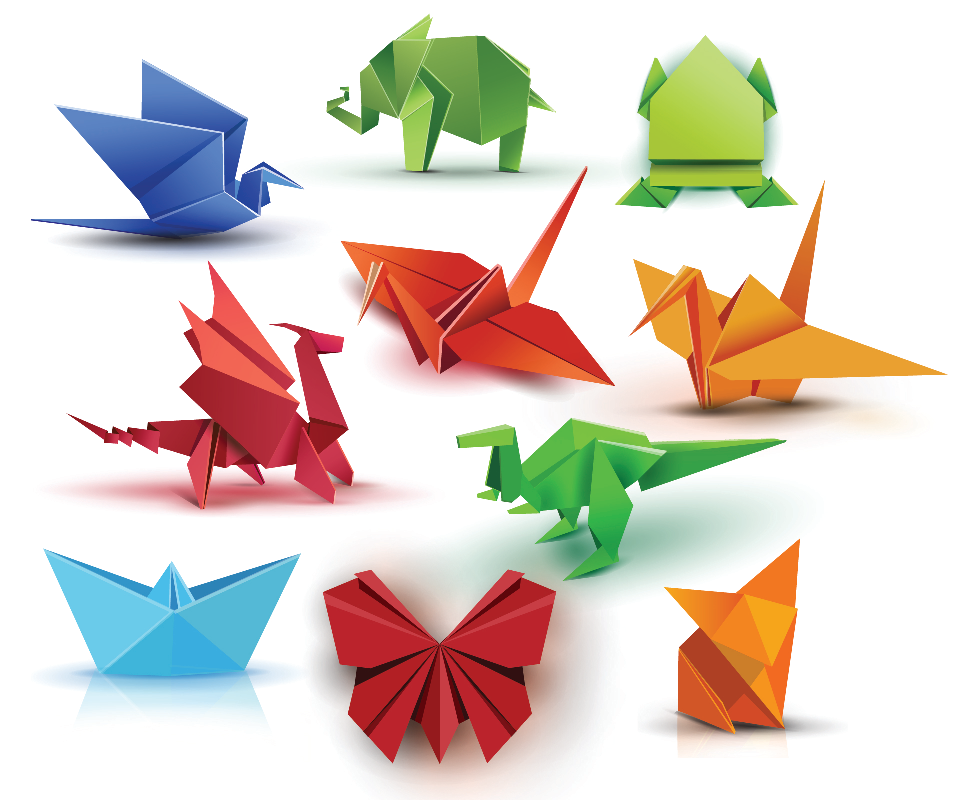
\includegraphics[width=1\linewidth]{figures/origami.pdf}
This result is known as the {\em Embedding Theorem}, due to 
\cite{nash1971imbedding}.
%John Forbes Nash, who became a household name after the Hollywood movie The Beautiful Mind. 
The %paper folding 
art of origami is a manifestation of different isometric embeddings of the planar surface in $\mathbb{R}^3$ (Figure: Shutterstock/300 librarians). 
}  If such functions can be expressed in terms of intrinsic quantities, they are automatically guaranteed to be isometry-invariant and thus unaffected by isometric deformations. 
%
These results can be further extended to dealing with approximate isometries; this is thus an instance of the geometric stability (domain deformation) discussed in our blueprint. 


%\taco{Taco: here we should probably make clear that we are not talking about symmetries in the sense of automorphisms, i.e. maps $\Omega \rightarrow \Omega$ that preserve the metric, but about isomorphisms, i.e. maps $\Omega \rightarrow \Omega'$ that preserve the metric. Note that we do not yet discuss this in the template, but as discussed we should.} 

%\michael{Approx isometry - geometric stability}

While, as we noted, the definition of a Riemannian manifold does not require a
geometric realisation in any space, it turns out that any smooth Riemannian manifold can be realised as a subset of a Euclidean space of sufficiently high dimension (in which case it is said to be `embedded' in that space) by using the structure of the Euclidean space to induce a Riemannian
metric. Such an embedding is however not necessarily unique -- as we will see, two different isometric 
realisations of a Riemannian metric are possible. 
%called {\em isometries}.



%\joan{Consider a transition paragraph here, where we explain that we introduce the minimal elements of differential geometry that lead to the key notion of isometry and geodesics}



\paragraph{Scalar and Vector fields}
%
Since we are interested in signals defined on $\Omega$, we need to provide the proper notion of scalar-
%\marginnote{We will use the same notation for tangent and vector fields, the distinction between which will be clear from the context.} 
and vector-valued functions on manifolds. 
%
A (smooth) {\em scalar field} is a function of the form $x: \Omega\rightarrow \mathbb{R}$. \marginnote{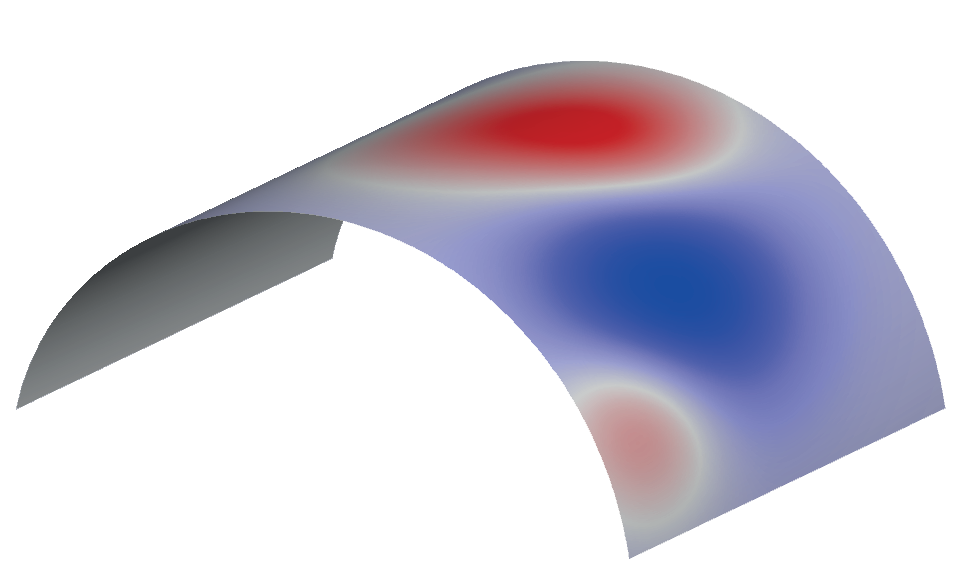
\includegraphics[width=0.9\linewidth]{figures/field_scalar.pdf}\\
Example of a scalar field. 
}
%\marginnote{The fields are typically assumed to be of the same regularity class (smoothness) as the manifold itself. }
%
%scalar-valued function  (often called a {\em scalar field}) $x: \Omega\rightarrow \mathbb{R}$ on the manifold. The space of 
Scalar fields form a vector space $\mathcal{X}(\Omega, \mathbb{R})$ that can be equipped with the inner product %of scalar fields
\begin{equation}
\langle x, y \rangle = \int_\Omega x(u) y(u) \mathrm{d}u,
\label{eq:inner_scalar}   
\end{equation}
%
where $\mathrm{d}u$ % = \sqrt{\det g}$
%\marginnote{More rigorously speaking, the volume form requires an inner product (i.e. Riemannian metric) and {\em orientation} (`handedness'). } 
is the volume element induced by the Riemannian metric. 
%
%
A (smooth) {\em tangent vector field} is a function of the form $X: \Omega \rightarrow T\Omega$  assigning to each point a tangent vector in the respective tangent space, $u\mapsto X(u)\in T_u\Omega$.  
%
Vector fields\marginnote{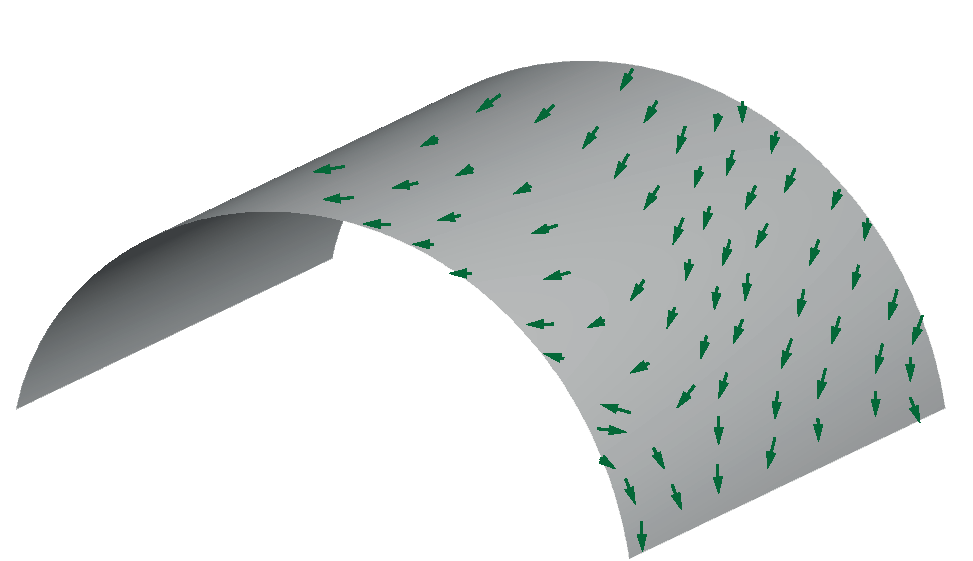
\includegraphics[width=0.9\linewidth]{figures/field_vector.pdf}\\
Example of a vector field. The fields are typically assumed to be of the same regularity class (smoothness) as the manifold itself.
} also form a vector space $\mathcal{X}(\Omega, T\Omega)$ with the inner product defined through the Riemannian metric, 
%
\begin{equation}
\langle X, Y \rangle = \int_\Omega g_u(X(u), Y(u)) \mathrm{d}u. \label{eq:inner_vector}   
\end{equation}


\paragraph{Intrinsic gradient}
Another way to think of (and actually {\em define}) vector fields is as a generalised notion of derivative. 
%
In classical calculus, one can locally linearise a (smooth) function through the {\em differential} $\mathrm{d}x(u) = x(u+\mathrm{d}u) - x(u)$, which provides the change of the value of the function $x$ at point $u$ as a result of an inifinitesimal displacement $\mathrm{d}u$. 
%
However, in our case the na{\"i}ve use of this definition is impossible, since 
%brings up two problems: First, 
expressions of the form ``$u+\mathrm{d}u$'' are meaningless on manifolds due to the lack of a global vector space structure. 
%, preventing us from adding or subtracting two points on $\Omega$. 
%
%
%A second problem arises when trying to take derivatives of vector fields, as one would need to subtract vectors belonging to tangent spaces at {\em different points}, while subtraction is only define \emph{within} a single vector space. 





The solution is %to the first problem is 
to use tangent vectors as a model of local infinitesimal displacement. 
%in order to provide a proper generalization of the differential on manifolds. 
%
Given a smooth scalar field $x\in \mathcal{X}(\Omega,\mathbb{R})$, we can think of a (smooth) vector field as a linear map $Y:\mathcal{X}(\Omega,\mathbb{R}) \rightarrow \mathcal{X}(\Omega,\mathbb{R})$ satisfying the properties of a {\em derivation}: 
$Y(c) = 0$ for any constant $c$ (corresponding to the intuition that constant functions have vanishing derivatives), $Y(x+z) = Y(x) + Y(z)$ (linearity), and $Y(xz) = Y(x)z + xY(z)$ ({\em product} or {\em Leibniz rule}), for any smooth scalar fields $x,z \in \mathcal{X}(\Omega,\mathbb{R})$. 
%
It can be shown that one can use these properties to define vector fields axiomatically. 
%
The differential $\mathrm{d}x(Y) = Y(x)$ 
can be viewed as an operator $(u,Y) \mapsto Y(x)$   
%
%defined as an operator $\mathrm{d}x : T\Omega \rightarrow \mathbb{R}$ of the form
%$$
%\mathrm{d}x(Y) = Y(x),
%$$
%which can be 
and interpreted as follows: the change of $x$ as the result of displacement $Y \in T_u\Omega$ at point $u$ is given by $\mathrm{d}_ux(Y)$. \marginnote{Importantly, this construction {\em does not use the Riemannian metric whatsoever} and can thus can be extended to a more general construction of bundles discussed in the Section~\ref{sec:gauges}. }
%
It is thus an extension of the classical notion of {\em directional derivative}. 
%



Alternatively, at each point $u$ the differential  can be regarded as a {\em linear functional} $\mathrm{d}x_u : T_u\Omega \rightarrow \mathbb{R}$ acting on tangent vectors $X \in T_u\Omega$. Linear functionals on a vector space are called {\em dual vectors} or {\em covectors}; if in addition we are given an inner product (Riemannian metric), a dual vector can always be represented as 
$$
\mathrm{d}x_u (X)  = g_u(\nabla x(u), X).\marginnote{This is a consequence of the Riesz-Fr{\'e}chet Representation Theorem, by which every dual vector can be expressed as an inner product with a vector. } 
$$ 
The representation of the differential at point $u$ is a tangent vector $\nabla x(u) \in T_u \Omega$ called the (intrinsic) {\em gradient} of $x$; similarly to the gradient in classical calculus, it can be thought of as the direction of the steepest increase of $x$. 
%
The gradient considered as an {\em operator} $\nabla : \mathcal{X}(\Omega,\mathbb{R}) \rightarrow \mathcal{X}(\Omega,T\Omega)$ assigns at each point $x(u) \mapsto \nabla x(u) \in T_u \Omega$; thus, the gradient of a scalar field $x$ is a vector field $\nabla x$. 
%As we will see later, this construction will allow us to generalise the notion of Fourier transform to manifolds. 

%More generally, the gradient can be thought of as an operator $\nabla : $



%In other words, the gradient produces a tangent vector field indicating the local direction of steepest increase of a scalar field on the manifold. 





%\taco{I think the notion of Torsion will be difficult to understand for newbies. Also, we are differentiating a tensor field g which I think we have not explained yet.

%We could consider just mentioning the LC connection and explaining that parallel transport defined wrt it will not change the length of tangent vectors. We can also say that if another condition (Torsion free) is satisfied, there is a unique LC connection, without formalizing it.}



\paragraph{Geodesics}

Now consider a smooth curve $\gamma : [0,T] \rightarrow \Omega$ on the manifold with endpoints $u = \gamma(0)$ and $v = \gamma(T)$. The derivative of the curve at point $t$ is a tangent vector $\gamma'(t) \in T_{\gamma(t)}\Omega$ called the {\em velocity vector}. \marginnote{It is tacitly assumed that curves are given in {\em arclength parametrisation}, such that $\| \gamma' \| = 1$ (constant velocity).} 
%
Among all the curves connecting points $u$ and $v$, we are interested in those of {\em minimum length}, i.e., we are seeking $\gamma$ minimising the length functional 
%
$$
\ell(\gamma) = \int_{0}^T \| \gamma'(t) \|_{\gamma(t)} \mathrm{d}t =  \int_{0}^T g_{\gamma(t)}^{1/2} (\gamma'(t), \gamma'(t)) \mathrm{d}t. 
$$
%
Such curves are called {\em geodesics} (from the Greek \textgreek{geodai\textsigma{}{\'i}a}, literally `division of Earth') and they play important role in differential geometry. 
%
%
Crucially to our discussion, the way we defined geodesics is intrinsic, as they depend solely on the Riemannian metric (through the length functional). 


Readers familiar with differential geometry might recall that geodesics are a more general concept and their definition in fact does not necessarily require a Riemannian metric but a {\em connection} (also called a {\em covariant derivative}, as it generalises the notion of derivative to vector and tensor fields), which is defined axiomatically, similarly to our construction of the differential. 
%
Given a Riemannian metric, there exists a unique special connection called the\marginnote{The Levi-Civita connection is torsion-free and compatible with the metric. The Fundamental Theorem of Riemannian geometry guarantees its existence and uniqueness. } {\em Levi-Civita connection}  which is often tacitly assumed in Riemannian geometry. Geodesics arising from this connection are the length-minimising curves we have defined above. 


We will show next how to use geodesics to define a way to transport tangent vectors on the manifold (parallel transport), create local intrinsic maps from the manifold to the tangent space (exponential map), and define distances (geodesic metric). This will allow us to construct convolution-like operations by applying a filter locally in the tangent space. %
%among all curves with endpoints $u = \gamma(0)$ and $v=\gamma(T)$. 



\paragraph{Parallel transport}\marginnote{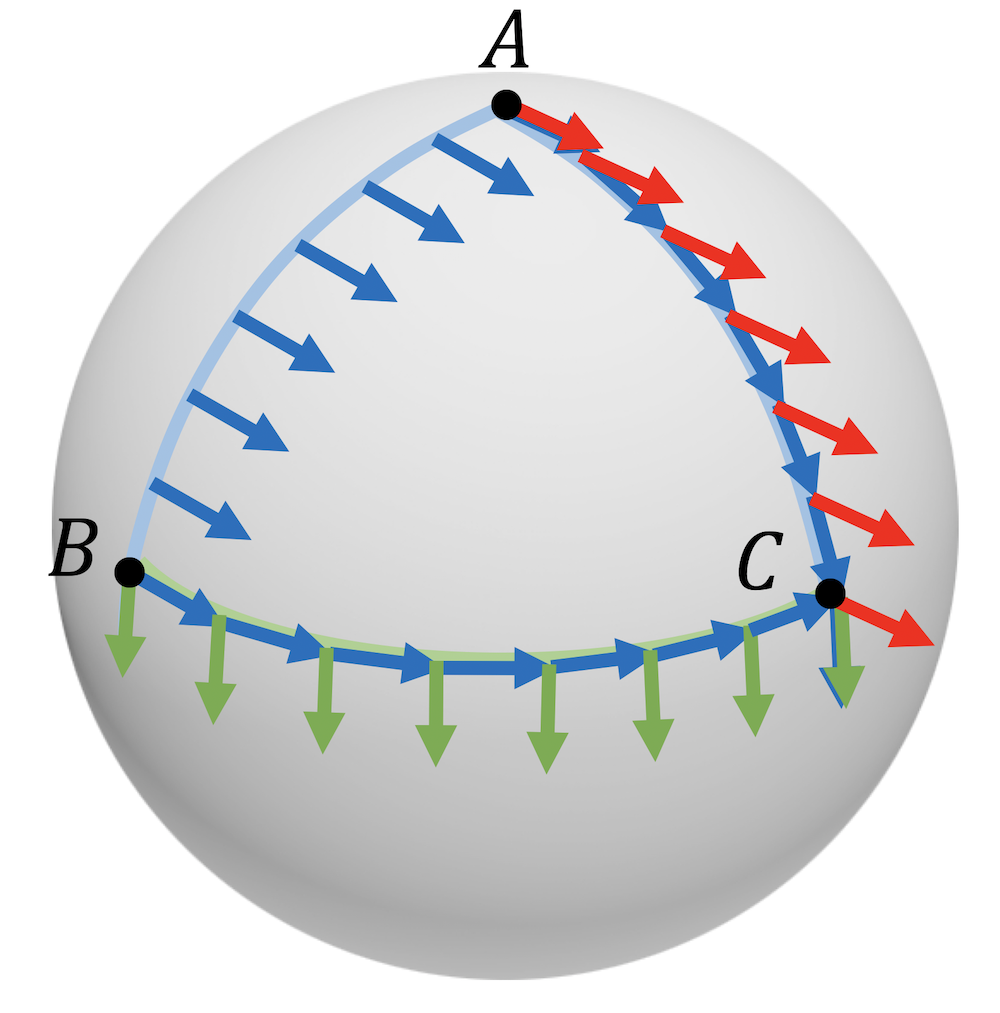
\includegraphics[width=0.9\linewidth]{figures/parallel.png}
Euclidean transport of a vector from A to C makes no sense on the sphere, as the resulting vectors (red) are not in the tangent plane. Parallel transport from A to C (blue) rotates the vector along the path. It is path dependent: going along the path BC and ABC produces different results.  
}
One issue we have already encountered when dealing with manifolds is that we cannot directly add or subtract two points $u,v \in \Omega$. 
%
The same problem arises when trying to compare tangent vectors at different points: though they have the same dimension, they belong to {\em different spaces}, e.g. $X\in T_u\Omega$ and $Y\in T_v\Omega$, and thus not directly comparable. 
%
Geodesics provide a mechanism to move vectors from one point to another, in the following way: let $\gamma$ be a geodesic connecting points $u=\gamma(0)$ and $v=\gamma(T)$ and let $X \in T_u\Omega$. We can define a new set of tangent vectors along the geodesic, $X(t) \in T_{\gamma(t)}\Omega$ such that the length of $X(t)$ and the angle (expressed through the Riemannian metric) between it and the velocity vector of the curve is constant,
$$
g_{\gamma(t)}(X(t),\gamma'(t) ) = g_{u}(X,\gamma'(0)) = \mathrm{const}, \quad\quad \|X(t)\|_{\gamma(t)} = \|X\|_u = \mathrm{const}.
$$
As a result, we get a unique vector $X(T) \in T_{v}\Omega$ at the end point $v$. %, which is unique. 


The map $\Gamma_{u\rightarrow v}(X) : T_u\Omega \rightarrow T_u\Omega$ and $T_v\Omega$ defined as $\Gamma_{u\rightarrow v}(X) = X(T)$ using the above notation is called {\em parallel transport} or {\em connection}; the latter term implying it is a mechanism to `connect' between the tangent spaces $T_u\Omega$ and $T_v\Omega$. 
%
Due to the angle and length preservation conditions, parallel transport amounts to only rotation of the vector, so it can be associated with an element of the special orthogonal group $\mathrm{SO}(s)$ (called the {\em structure group} of the tangent bundle),\marginnote{Assuming that the manifold is orientable, otherwise $\mathrm{O}(s)$.} which we will denote by $\fg_{u\rightarrow v}$ and 
discuss in further detail in Section~\ref{sec:gauges}. 

As we mentioned before,  a connection can be defined axiomatically independently of the Riemannian metric, providing thus an abstract notion of parallel transport along any smooth curve. The result of such transport, however, depends on the path taken.  
%As a general comment, parallel transport can be defined along any cur

%or {\em connection} 




\paragraph{Exponential map}
Locally around a point $u$, it is always possible to define a unique geodesic in a given direction $X \in T_u\Omega$, i.e. such that %a smooth curve $\gamma_X : [0,T] \rightarrow \Omega$ satisfying 
$\gamma(0) = u$ and $\gamma'(0) = X$. %, for some small $T>0$. 
%
%
When $\gamma_X(t)$ is defined for all $t\geq 0$ (that is, we can shoot the geodesic from a point $u$ for as long as we like), the manifold is said to be {\em geodesically complete} and the exponential map is defined on the whole tangent space.
%
Since compact manifolds are geodesically complete, we can tacitly assume this convenient property. 



%
This definition of geodesic provided a point and a direction gives a natural mapping from (a subset of) the tangent space $T_u \Omega$ to $\Omega$ called the {\em exponential map}\marginnote{
%Here, $B_\delta(0)$ is a ball of radius $\delta$ around the origin. 
Note that geodesic completeness does not necessarily guarantee that $\exp$ is a global diffeomorphism -- the largest radius $r$ about $u$ for which $\exp_u(B_r(0) \subseteq T_u\Omega)$ is mapped diffeomorphically is called the {\em injectivity radius}. }  $\exp : B_r(0) \subset T_u\Omega \rightarrow \Omega$, which is defined by taking a unit step along the geodesic in the direction $X$, i.e., $\exp_u(X) = \gamma_X(1)$. %
%
The exponential map $\exp_u$ is a local diffeomorphism, as it deforms the neighbourhood $B_r(0)$ (a ball or radius $r$) of the origin on $T_u\Omega$ into a neighbourhood of $u$. Conversely, one can also regard the exponential map as an intrinsic local deformation (`flattening') of the manifold into the tangent space. 




\paragraph{Geodesic distances}
%
A result known as the Hopf-Rinow Theorem 
%
\marginnote{Hopf-Rinow Theorem thus estabilishes the equivalence between geodesic and metric completeness, the latter meaning every Cauchy sequence converges in the geodesic distance metric.} guarantees that geodesically complete manifolds are also {\em complete metric spaces}, in which one can realise a distance (called the {\em geodesic distance} or {\em metric})  between any pair of points $u,v$ as the length of the shortest path between them
$$
d_g(u,v) = \min_{\gamma} \ell(\gamma) \quad\quad \text{s.t.} \quad\quad \gamma(0) = u, \,\, \gamma(T) = v,
$$
which exists (i.e., the minimum is attained).\marginnote{Note that the term `metric' is used in two senses: Riemannian metric $g$ and distance $d$. To avoid confusion, we will use the term `distance' referring to the latter. Our notation $d_g$ makes the distance depend on the Riemannian metric $g$, though the definition of geodesic length $L$. }



%The term `geodesic' is also used in metric geometry, where it is defined as the shortest path. In the setting described here the two meanings coincide. }


%i.e., the two notions of `geodesic' used somewhat differently in differential and metric geometry







\paragraph{Isometries}
Consider now a deformation of our manifold $\Omega$ into another manifold $\tilde{\Omega}$ with a Riemannian metric $h$, which we assume to be 
%
%We will assume this map to be 
a diffeomorphism $\eta: (\Omega, g) \rightarrow (\tilde{\Omega}, h)$ between the manifolds.   
%
Its differential $\mathrm{d}\eta : T\Omega \rightarrow T\tilde{\Omega}$ defines a map between the respective tangent bundles (referred to as {\em pushforward}), such that   
%\marginnote{The pushforward is what is called a {\em bundle map}.}
at a point $u$, we have $\mathrm{d}\eta_u : T_u \Omega \rightarrow T_{\eta(u)}\tilde{\Omega}$, %which allows to interpret it as follows: 
%
interpreted as before: 
if we make a small displacement from point $u$ by tangent vector $X \in T_u \Omega$, the map $\eta$ will be displaced from point $\eta(u)$ by tangent vector $\mathrm{d}\eta_u(X) \in T_{\eta(u)}\tilde{\Omega}$. 


Since the pushforward\marginnote{Pushforward and pullback are adjoint operators $\langle \eta^* \alpha, X \rangle = \langle \alpha, \eta_*X \rangle$ where $\alpha \in T^*\Omega$ is a {\em dual vector field}, defined at each point as a linear functional acting on $T_u\Omega$ and the inner products are defined respectively on vector and dual vector fields. } provides a mechanism to associate tangent vectors on the two manifolds, it allows to {\em pullback } the metric $h$ from $\tilde{\Omega}$ to $\Omega$, 
$$
(\eta^*h)_u(X,Y) = h_{\eta(u)}(\mathrm{d}\eta_u(X), \mathrm{d}\eta_u(Y))
$$ 
%
If the pullback metric coincides at every point with that of $\Omega$, i.e., $g = \eta^*h$, the map $\eta$ is called  (a Riemannian) {\em isometry}. % (metric-preserving). 
%
For two-dimensional manifolds (surfaces), isometries can be intuitively understood as inelastic deformations that deform the manifold without `stretching' or `tearing' it. 



By virtue of their definition, isometries preserve intrinsic structures such as geodesic distances, which are expressed entirely in terms of the Riemannian metric. % and Gaussian curvature.
%
Therefore, we can also understand isometries from the position of metric geometry, 
 as distance-preserving maps (`metric isometries') {\em between metric spaces} $\eta : (\Omega, d_g) \rightarrow (\tilde{\Omega}, d_h)$, in the sense that 
$$
d_g (u,v) = d_h(\eta(u),\eta(v)) 
$$
for all $u,v \in \Omega$, 
or more compactly, $d_g = d_h \circ (\eta \times \eta)$. In other words, Riemannian isometries are also metric isometries. 
%
On {\em connected} manifolds, the converse is also true: every metric isometry is also a Riemannian isometry. 
\marginnote{This result is known as the Myers–Steenrod Theorem. We tacitly assume our manifolds to be connected. }
%where $d_g, d_g$ are the geodesic distances induced by the respective Riemannian metrics $g, h$. 


In our Geometric Deep Learning blueprint, $\eta$ is a model of domain deformations. When $\eta$ is an isometry, %(roughly, an inelastic deformation that does not `stretch' the manifold), 
any intrinsic quantities are unaffected by such deformations. 
%
%This is the reason why we insist on working with structures defined intrinsically. 
%
One can generalise exact (metric) isometries through the notions of %this notion 
{\em metric dilation} 
$$
\mathrm{dil}(\eta) = \sup_{u\neq v \in \Omega}\frac{d_h(\eta(u),\eta(v))}{d_g (u,v)}
$$
%
or {\em metric distortion} 
$$
\mathrm{dis}(\eta) = \sup_{u, v \in \Omega}|d_h(\eta(u),\eta(v)) - d_g (u,v)|,
\marginnote{The Gromov-Hausdorff distance
%\marginnote{
%More precisely, $d_{\mathrm{GH}}(\Omega,\Omega') = \frac{1}{2}\inf_{(x,y) \in C} %\mathrm{dis}$
%} 
between metric spaces, which we mentioned in Section~\ref{sec:isomorphism}, can be expressed as the smallest possible metric distortion.}
$$
which capture the relative and absolute change of the geodesic distances under $\eta$, respectively. 
%
The condition~(\ref{eqn:domain_def_stability}) for the stability of a function $f \in \mathcal{F}(\mathcal{X}(\Omega))$ 
under domain deformation
can be rewritten in this case as 
$$
\| f(x,\Omega) - f(x\circ \eta^{-1},\tilde{\Omega})\| \leq C \|x\| \mathrm{dis}(\eta). 
$$


%[Gauss Theorema Egregium, definition of curvature through perimeter defect, pizza example]


\paragraph{Intrinsic symmetries}
A particular case of the above is a diffeomorphism  of the domain itself (what we termed {\em automorphism} in Section~\ref{sec:isomorphism}), which we will denote by $\tau \in \mathrm{Diff}(\Omega)$. We will call it a Riemannian  \mbox{(self-)isometry} if the pullback metric satisfies $\tau^* g = g$, or a metric (self-)isometry if $d_g = d_g\circ (\tau \times \tau)$.
%
Not surprisingly,\marginnote{Continuous symmetries on manifolds are infinitesimally generated by special tangent vector fields called {\em Killing fields}, named after Wilhelm Killing.} isometries form a group with the composition operator denoted by $\mathrm{Iso}(\Omega)$ and called the {\em isometry group}; the identity element is the map $\tau(u) = u$ and the inverse always exists (by definition of $\tau$ as a diffeomorphism). 
%
Self-isometries are thus {\em intrinsic symmetries} of manifolds.


%Continuous symmetries on manifolds are infinitesimally generated
%%\marginnote{More correctly, Killing fields are the infinitesimal generators of continuous symmetries. } 
%by special tangent vector fields called {\em Killing fields}, named after Wilhelm Killing. A field $X$ is Killing if the  Lie derivative\marginnote{The Lie derivative in this case is a derivative of forms. For scalar and vector fields, it coincides with the covariant derivative $\mathcal{L}_X y = \nabla_X y$ and the commutator $\mathcal{L}_X Y = [X,Y]$, respectively. } of the Riemannian metric along it vanishes, $\mathcal{L}_X g = 0$, which is interpreted as 
%%
%$$
%\mathcal{L}_X g(Y,Z) = g(\nabla_Y X, Z) + g(Y,\nabla_Z X) = 0
%$$
%for any smooth tangent fields $Y, Z$. 
%%
%We can recap that like we mentioned in Section~\ref{sec:symmetries}, we can regard symmetries as automorphisms (self-maps) preserving additional structure: either the local Riemannian metric, or global geodesic distances between pairs of points. 
%%\taco{Do we need Killing fields? It's interesting but I worry that we'd need to properly introduce Lie derivatives to make it understandable.} \michael{Lets keep them for now}
%%OK :)



\paragraph{Fourier analysis on Manifolds}
%Reconnecting to our Geometric Deep Learning blueprint, we now have a way to guarantee geometric stability by construction, considering intrinsic quantities expressed through the Riemannian metric. 
%
We will now show how to construct intrinsic convolution-like operations on manifolds, which, by construction, will be invariant to isometric deformations.    
For this purpose, 
%In order to define convolution-like operations, 
we have two options: One is to use an analogy of the Fourier transform, and define the convolution as a product in the Fourier domain. 
%
The other is to define the convolution spatially, by correlating a filter locally with the signal. 
%by ``shifting'' a filter around via parallel transport.
Let us discuss the spectral approach first.


We remind that in the Euclidean domain the Fourier transform is obtained as the eigenvectors of circulant matrices, which are jointly diagonalisable due to their commutativity. Thus, any circulant matrix and in particular, differential operator, can be used to define an analogy of the Fourier transform on general domains. 
%
In Riemannian geometry, it is common to use the orthogonal eigenbasis of the Laplacian operator, which we will define here. 


For this purpose, recall our definition of the intrinsic gradient operator $\nabla : \mathcal{X}(\Omega,\mathbb{R}) \rightarrow \mathcal{X}(\Omega,T\Omega)$, 
%assigning at each point $x(u) \mapsto \nabla x(u) \in T_u \Omega$. In other words, the gradient produces 
producing a tangent vector field that indicates the local direction of steepest increase of a scalar field on the manifold. 
%
In a similar manner, we can define the {\em divergence operator} $\nabla^* : \mathcal{X}(\Omega,T\Omega) \rightarrow \mathcal{X}(\Omega,\mathbb{R})$. 
%
If we think of a tangent vector field as a
flow on the manifold, the divergence measures
the net flow of a field at a point, allowing to distinguish
between field `sources' and `sinks'. 
%
We use the notation $\nabla^*$ (as opposed to the common $\mathrm{div}$) to emphasise that the two operators are adjoint,
$$
\langle X, \nabla x\rangle = \langle \nabla^* X,  x\rangle,
$$
where we use the inner products (\ref{eq:inner_scalar}) and~(\ref{eq:inner_vector}) between scalar and vector fields. 
%with the inner products defined on vector and scalar fields, respectively. 

The {\em Laplacian} (also known as the {\em Laplace-Beltrami operator} in differential geometry) is an operator on $\mathcal{X}(\Omega)$ defined as $\Delta = \nabla^* \nabla$,  
%; as opposed to most of the textbooks, we use the negative sign to ensure our operator is positive semi-definite. 
%
which can be interpreted \marginnote{From this interpretation it is also clear that the Laplacian is isotropic. We will see in Section~\ref{sec:meshes} that it is possible to define {\em anisotropic Laplacians} (see \citep{andreux2014anisotropic,boscaini2016anisotropic}) of the form $\nabla^*(A(u)\nabla)$, where $A(u)$ is a position-dependent tensor determining local direction. 
%In practice, such a construction requires a fixed gauge. 
}
%For the classical Euclidean Laplacian defined as the sum of second-order derivatives this can be seen by writing it as the trace of the Hessian, $\Delta x(\mathbf{u})= \mathrm{trace} \nabla^2 x(\mathbf{u})$, applying an orthogonal transformation of coordinates $\mathbf{u}\mapsto \mathbf{Ru}$,  and using the chain rule.
%}
as the difference between the average of a function on an
infinitesimal sphere around a point and the value of the
function at the point itself. 
%
%
It is one of the most important operators in mathematical physics, used to describe phenomena as diverse as heat diffusion, quantum oscillations,
and wave propagation.  
%
Importantly in our context, the Laplacian is intrinsic, and thus invariant under isometries of $\Omega$. 



It is easy to see that the Laplacian is self-adjoint (`symmetric'),
$$
\langle \nabla x, \nabla x \rangle = \langle x , \Delta x\rangle = \langle \Delta x ,  x\rangle.
$$
The quadratic form on the left in the above expression is actually the already familiar Dirichlet energy,  
$$c^2(x) = \| \nabla x \|^2 = \langle \nabla x, \nabla x \rangle = \int_\Omega \| \nabla x(u) \|_u^2 \mathrm{d}u = \int_\Omega g_u( \nabla x(u),  \nabla x(u)) \mathrm{d}u
$$
measuring the smoothness of $x$. 
%As we will see in the following, the Laplacian plays a center role in signal processing and learning on non-Euclidean domains, as its eigenfunctions generalize the classical Fourier bases, allowing to perform spectral analysis on manifolds and graphs
%
%
%
%
%allowing to interpret it as the smoothest orthogonal basis. 
%
%
%We will discuss this construction in detail in Chapter ???, where we will show that Laplacian eigenvalues and eigenvectors capture important geometric properties of the manifold. 



The Laplacian operator admits an eigedecomposition %eigenfunctions
$$
\Delta \varphi_k = \lambda_k \varphi_k, \quad\quad k=0, 1, \hdots 
$$
%
%which is discrete 
with countable spectrum if the manifold is compact (which we tacitly assume), and orthogonal eigenfunctions, $\langle \varphi_k, \varphi_l \rangle = \delta_{kl}$, due to the self-adjointness of $\Delta$. 
%discrete on compact manifolds
%orthogonal since $\Delta$ is self-adjoint
%
The Laplacian eigenbasis can also be constructed as a set of orthogonal minimisers of the Dirichlet energy, 
$$
\varphi_{k+1} = \arg\min_{\varphi} \| \nabla \varphi \|^2      \quad\quad \text{s.t.}\quad\quad   \|\varphi \|=1 \,\,\, \text{and} \,\,\, \langle \varphi, \varphi_{j} \rangle = 0 
$$
for $j=0,\hdots, k$, allowing to interpret it as the smoothest orthogonal basis on $\Omega$. 
%
The eigenfunctions $\varphi_0, \varphi_1, \hdots$ and the corresponding eigenvalues $0 = \lambda_0 \leq \lambda_1 \leq \hdots $ can be interpreted as the analogy of the atoms and frequencies in the classical Fourier transform. \marginnote{In fact $e^{\mi \xi u}$ are the eigenfunctions of the Euclidean Laplacian $\tfrac{\mathrm{d}^2}{\mathrm{d} u^2}$.}
%


This orthogonal basis allows to expand square-integrable functions on $\Omega$ into {\em Fourier series}  
$$
x (u) = \sum_{k \geq 0} \langle x, \varphi_k \rangle \varphi_k (u)
$$
%
where $\hat{x}_k = \langle x, \varphi_k \rangle$ are referred to as the {\em Fourier coefficient} or the (generalised) Fourier transform of $x$. \marginnote{Note that this Fourier transform has a discrete index, since the spectrum is discrete due to the compactness of $\Omega$.}
%
Truncating the Fourier series results in an approximation error that can be bounded \citep{aflalo2013spectral} by 
$$
\left\| x - \sum_{k = 0}^N \langle x, \varphi_k \rangle \varphi_k \right\|^2 \leq \frac{\| \nabla x\|^2}{\lambda_{N+1}}.
$$
\cite{aflalo2015optimality} further showed that no other basis attains a better error, making the Laplacian eigenbasis  {\em optimal} for representing smooth signals on manifolds. 


\paragraph{Spectral Convolution on Manifolds}
%Let us now remind the reader that we defined Euclidean convolution in Section~\ref{sec:groups} as inner product with a shifted filter $(x \star \psi)(u) =  \langle x, T_u \psi \rangle$. This construction had two important properties, linearity and commutativity, that works in both ways, allowing to {\em define} convolution as a linear operator that commutes with shift. 
%%
%On a manifold, because we lack a global vector space structure, we cannot immediately define the shift operator $(T_v x)(u) = x(u-v)$ since ``$u-v$'' makes no sense. 
%%
%However, we can keep $T_u$ as an abstract linear operator and use the above two properties as a definition. 
%
%
%First, we note that commutativity implies 
%$$
%(T_v (x\star \psi))(u) = \langle x, T_v T_u \psi \rangle =  \langle T_v x, T_u  \psi \rangle = ((T_v x)\star \psi)(u).  
%$$
%%
%Expressing each of the functions %$x$, $T_u \psi$, and $T_v x$ 
%in the Fourier basis allows us to rewrite %this identity as 
%\begin{eqnarray*}
%\langle T_v x, T_u\psi \rangle &=& \left \langle 
%\sum_{k\geq 0} \langle T_v x,\varphi_k \rangle \varphi_k \,, \,\,
%\sum_{l\geq 0} \langle T_u\psi,\varphi_l \rangle \varphi_l
%\right \rangle \\
%&=& \sum_{k,l\geq 0} \langle T_v x,\varphi_k \rangle \langle T_u\psi,\varphi_l \rangle \langle \varphi_k, \varphi_l \rangle \\
%&=& \sum_{k \geq 0} \langle T_v x,\varphi_k \rangle \langle T_u\psi,\varphi_k \rangle, \marginnote{We use here the orthogonality of the basis, $\langle \varphi_k, \varphi_l \rangle = \delta_{kl}$.}
%\end{eqnarray*}
%%
%and similarly, 
%$
%\langle x, T_v T_u\psi \rangle =
%\sum_{k \geq 0} \langle x,\varphi_k \rangle \langle T_v  T_u\psi,\varphi_k \rangle
%$,
%%
%from where the spectral expression of the commutativity condition follows:
%$$
%\langle T_v x,\varphi_k \rangle \langle T_u\psi,\varphi_k \rangle 
%= \langle x,\varphi_k \rangle \langle T_v  T_u\psi,\varphi_k \rangle \quad\quad \text{for all} \, k\geq 0.
%$$
%In particular, for $x=\psi = \varphi_l$ we get 
%$
%\langle T_v \varphi_l,\varphi_k \rangle \langle T_u \varphi_l,\varphi_k \rangle 
%= \delta_{kl} \langle T_v  T_u \varphi_l,\varphi_k \rangle 
%$
%which leads us to $\langle T_v \varphi_l,\varphi_k \rangle = 0$ for $k\neq l$. This means that Fourier basis functions are the eigenfunctions of the shift operator, like we had in the Euclidean case,  i.e., $T_v \varphi_k = \mu_v \varphi_k$.
%
%
%In order to determine the eigenvalues $\mu_v$, we consider again the commutativity condition with $x=\varphi_k$ and $\psi = \delta_u$ the Dirac delta function\marginnote{The {\em Dirac delta} or {\em impulse function} is defined as $\langle \delta_u , x \rangle = x(u)$. It can thus be considered as the representation of the linear functional (dual vector) $x \mapsto x(u)$.  } 
%
%
%
%Second, using  the linearity of $T_v$, we get 
%%the general expression  
%$$
%(T_v x)(u) = \sum_{k\geq 0} \langle x, \varphi_k\rangle (T_v \varphi_k) (u)
%= \sum_{k\geq 0} \langle x, \varphi_k\rangle  \varphi_k (v) \varphi_k (u)
%= \sum_{k\geq 0} \hat{x}_k  \varphi_k (v) \varphi_k (u), 
%%\marginnote{In the Euclidean case, one has (from the associativity of exponents and complex conjugation in the inner product) $\varphi_i (v) \bar{\varphi}_i (u) = \varphi_i (v - u)$. In the general case, the shift operator is thus position-dependent and the signal is {\em changed} when shifted.  }
%$$
%which is a non-Euclidean generalisation of the shift operator. 
%%
%It is easy to verify that in the Euclidean case, $\Omega = [0,L]$, \marginnote{ Here we assume a compact interval, in which case the Fourier basis is discrete. Note that the shift we get is $x(u+v)$ rather than $x(u-v)$, which is just notational difference.}  where the Fourier basis is of the form $\varphi_k(u) = e^{\mi \frac{2\pi k}{L} u}$, we get the familiar expression 
%$$
%(T_v x)(u) = \sum_{k\geq 0} \hat{x}_k e^{\mi \frac{2\pi k}{L} v} e^{\mi \frac{2\pi k}{L} u} 
%\sum_{k\geq 0} \hat{x}_k e^{\mi \frac{2\pi k}{L} (u+v)} = x(u+v).
%$$
%
%
%Finally, plugging the expression of $T_u$ into the definition of convolution, we get
%%{\em spectral convolution}
%%
%\begin{eqnarray}
%(x \star \psi)(u) &=& \langle x, T_u \psi \rangle = 
%\left \langle x, \, \sum_{k\geq 0} \hat{\psi}_k \varphi_k(u) \phi_k 
%\right\rangle \nonumber \\
%&=&
%\sum_{k \geq 0} \langle x, \varphi_k \rangle \hat{\psi}_k  \varphi_k (u)  = \sum_{k \geq 0} (\hat{x}_k \cdot \hat{\psi}_k ) \varphi_k (u).
%\label{eqn:conv_spectral}
%\end{eqnarray}
%%
%%In a sense, we used what was a {\em property} of the classical Fourier transform (the Convolution Theorem) as a way to {\em define} a non-Euclidean convolution. 
%%
%Expression~(\ref{eqn:conv_spectral}) is often called {\em spectral convolution}, since it coincides with the Convolution Theorem, expressing the convolution in spectral domain as the point-wise product of the Fourier transforms $\hat{\psi}_k$ and $\hat{x}_k$.  
%%
%This construction is usually motivated by using a {\em property} of the classical Fourier transform (the Convolution Theorem) as a way to {\em define} a non-Euclidean convolution. However, here we have shown the derivation from first principles of shift equivariance (where the shift is understood in a more general sense). 
%%
%The key property of spectral convolution is that, by virtue of its construction, it is intrinsic and thus isometry-invariant. 




{\em Spectral convolution} can be defined as the product of Fourier transforms of the signal $x$ and the filter $\theta$, 
\begin{equation}
(x \star \theta)(u) = 
\sum_{k \geq 0} (\hat{x}_k \cdot \hat{\theta}_k ) \varphi_k (u).
\label{eqn:conv_spectral}
\end{equation}
%
Note that here we use what is a {\em property} of the classical Fourier transform (the Convolution Theorem) as a way to {\em define} a non-Euclidean convolution.
%
By virtue of its construction, the spectral convolution is intrinsic and thus isometry-invariant. 
%
Furthermore, since the Laplacian operator is isotropic, it has no sense of direction; in this sense, the situation is similar to that we had on graphs in Section~\ref{sec:proto-graphs} due to permutation invariance of neighbour aggregation. 







\begin{figure}[h!]
    \centering
    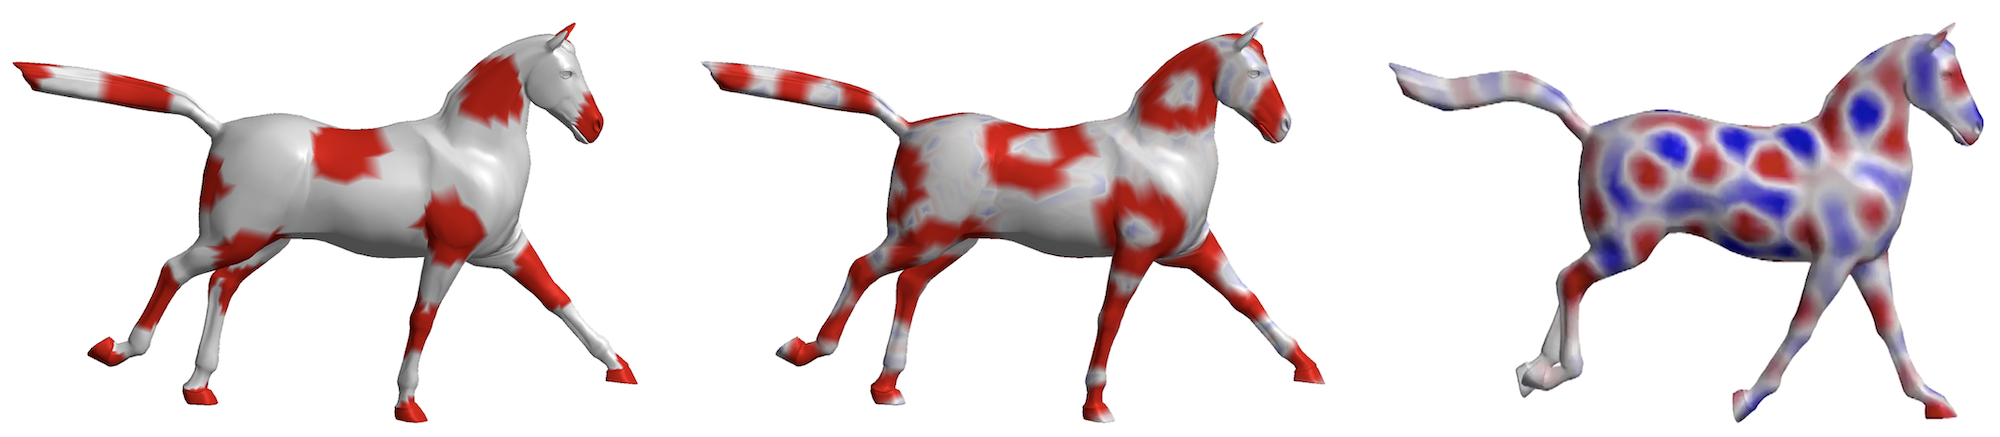
\includegraphics[width=\linewidth]{figures/horses.png}
    \caption{Instability of spectral filters under domain perturbation. Left: a signal $\mathbf{x}$ on the mesh $\Omega$. Middle: result of spectral filtering %$\mathbf{x}\star \boldsymbol{\theta} = \boldsymbol{\Phi}\, \mathrm{diag}(\hat{\boldsymbol{\theta}}) \boldsymbol{\Phi}^\top \mathbf{x}$ 
    in the eigenbasis %$\boldsymbol{\Phi}$ 
    of the Laplacian $\Delta$ on $\Omega$. 
    Right: 
    the same spectral filter %$\boldsymbol{\theta}$ 
    applied to the eigenvectors %$\bar{\boldsymbol{\Phi}}$ 
    of the Laplacian $\tilde{\Delta}$ of a nearly-isometrically perturbed domain $\tilde{\Omega}$ 
    %(as a result of a near-isometric deformation of the mesh)  
%    $\bar{\boldsymbol{\Phi}}\, \mathrm{diag}(\hat{\boldsymbol{\theta}}) \bar{\boldsymbol{\Phi}}^\top \mathbf{x}$
    produces a very different result. 
    }
    \label{fig:mesh_horses}
\end{figure}%




%
In practice, a direct computation of~(\ref{eqn:conv_spectral}) appears to be prohibitively expensive due to the need to diagonalise the Laplacian. Even worse, 
%, as we will see in Section~\ref{sec:meshes}, 
it turns out geometrically unstable: the higher-frequency eigenfunctions of the Laplacian can change dramatically as a result of even small near-isometric perturbations of the domain $\Omega$ (see Figure~\ref{fig:mesh_horses}). 
%
%
A more stable solution is provided by realising the filter as a {\em spectral transfer function} of the form $\hat{p}(\Delta)$, 
%which is understood in the operator sense as %\marginnote{Geometric Deep Learning methods based on spectral convolution expressed through the Fourier transform are often referred to as `spectral' and opposed to `spatial' methods we have seen before in the context of graphs. When expressed as spectral transfer function, the former in fact boil down to the latter, so this dichotomy is somewhat artificial and not completely appropriate.}
\begin{eqnarray}
(\hat{p}(\Delta) x)(u) &=& \sum_{k\geq 0} \hat{p}(\lambda_k) \langle x, \varphi_k\rangle \varphi_k (u) \label{eqn:conv_spec} \\
%
&=& \int_\Omega x(v) \, \sum_{k\geq 0} \hat{p}(\lambda_k) \varphi_k(v) \varphi_k (u) \, \mathrm{d}v \label{eqn:conv_spat}
\end{eqnarray}
%
which can be interpreted in two manners: either as a spectral filter~(\ref{eqn:conv_spec}), where we identify $\hat{\theta}_k = \hat{p}(\lambda_k)$, or as a spatial filter~(\ref{eqn:conv_spat}) with a position-dependent kernel $\theta(u,v) = \sum_{k\geq 0} \hat{p}(\lambda_k) \varphi_k(v) \varphi_k (u)$.  
%
%
The advantage of this formulation is that $\hat{p}(\lambda)$ can be parametrised by a small number of coefficients, and choosing parametric functions such as polynomials\marginnote{Geometric Deep Learning methods based on spectral convolution expressed through the Fourier transform are often referred to as `spectral' and opposed to `spatial' methods we have seen before in the context of graphs. We see here that these two views may be equivalent, so this dichotomy is somewhat artificial and not completely appropriate.} $\hat{p}(\lambda) = \sum_{l=0}^r \alpha_l \lambda^l$ allows for efficiently computing the filter as 
$$
(\hat{p}(\Delta) x)(u) = \sum_{k\geq 0} \sum_{l= 0}^r \alpha_l \lambda_k^l \, \langle x, \varphi_k\rangle \varphi_k (u) = \sum_{l= 0}^r \alpha_l (\Delta^l x)(u),
$$
avoiding the spectral decomposition altogether. 
%
We will discuss this construction in further detail in Section~\ref{sec:meshes}. 

%\michael{Add note on stability}

%While filters defined in this manner are isotropic (direction-unaware), 



\paragraph{Spatial Convolution on Manifolds}

A second alternative is to attempt defining convolution on manifolds is by matching a filter at different points, like we did in formula~(\ref{eq:group-conv}), 
%
\begin{equation}
(x \star \theta)(u) = \int_{T_u \Omega} x(\exp_u Y) \theta_u(Y) \mathrm{d}Y, 
\label{eq:conv_tangent_space}
\end{equation}
%
where we now have to use the exponential map to access the values of the scalar field $x$ from the tangent space, and 
the filter $\theta_u$ is defined in the tangent space at each point and hence position-dependent. %
If one defines the filter intrinsically, such a convolution would be isometry-invariant, a property we mentioned as crucial in many computer vision and graphics applications. 
%, and we use the exponential map to obtain. 


We need, however, to note several substantial differences from our previous construction in Sections~\ref{sec:grids_euclidean}--\ref{sec:groups}. 
%
First, because a manifold is generally not a homogeneous space, we do not have anymore a global group structure allowing us have a shared filter (i.e., the same $\theta$ at every $u$ rather than $\theta_u$ in expression~(\ref{eq:conv_tangent_space})) defined at one point and then move it around. 
%as we did in formula~(\ref{eq:group-conv}). 
%
An analogy of this operation on the manifold would require parallel transport, allowing to apply a shared $\theta$, defined as a function on $T_u\Omega$, at some other $T_v\Omega$.   
%
However, as we have seen, this in general will depend on the path between $u$ and $v$, so {\em the way we move the filter around matters.}%\marginnote{As a possible remedy, \cite{poulenard2018multi} suggested moving the filter along geodesics. } 
%
%
Third, since we can use the exponential map only locally, the filter must be {\em local}, with support bounded by the injectivity radius.  
%
Fourth 
and most crucially, we cannot work with $\theta(X)$, as $X$ is an abstract geometric object: in order for it to be used for computations, we must represent it {\em relative to some local basis}  
$\omega_u : \mathbb{R}^s \rightarrow T_u\Omega$, as an $s$-dimensional array of coordinates $\mathbf{x} = \omega^{-1}_u(X)$. 
%
This allows us to rewrite the convolution~(\ref{eq:conv_tangent_space}) as 
%
\begin{equation}
(x \star \theta)(u) = \int_{[0,1]^s} x(\exp_u (\omega_u \mathbf{y})) \theta(\mathbf{y}) \mathrm{d}\mathbf{y}, 
\label{eqn:conv_exp}
\end{equation}
%

%\joan{We have used $\delta$ in the previous sections to refer to the size of the filter support}

with the filter defined on the unit cube. Since the exponential map is intrinsic (through the definition of geodesic), the resulting convolution is isometry-invariant. 


Yet, this tacitly assumed  we can carry the frame $\omega_u$ along to another manifold, i.e. $\omega_u' = \mathrm{d}\eta_u \circ \omega_u$.
%
%Yet, we should point to one issue that at a close inspection opens a can of worms: in our definition, we assumed $\omega$ was given, which 
Obtaining
such a frame (or \emph{gauge}, in physics terminology) given only a the manifold $\Omega$ in a consistent manner is however fraught with difficulty.
%implies that we need some mechanism to {\em fix a basis at each point} of the manifold (in physics, a smooth choice of local bases is referred to as a {\em gauge}). 
%
First, a smooth global gauge may not exist: this is the situation on manifolds that are not \emph{parallelisable},\marginnote{The sphere $\mathbb{S}^2$ is an example of a non-parallelisable manifold, a result of    
%on which one cannot construct a smooth tangent vector field. 
the {\em Poincar{\'e}-Hopf Theorem}, which is colloquially stated as `one cannot comb a hairy ball without creating a cowlick.' \vspace{2mm}
%and is the reason why magnetic plasma confinement chambers must have toroidal rather than spherical geometry. 
%\includegraphics[width=1\linewidth]{figures/hairy_ball.png}
}   in which case one cannot define a smooth non-vanishing tangent vector field.
%; we further assume that the global gauge is smooth, which is only possible if the manifold is {\em parallelizable}.
%
%
Second, we do not have a canonical gauge on manifolds, so this choice is arbitrary; since our convolution depends on $\omega$, if one chose a different one, we would obtain different results. 

We should note that this is a case where practice diverges from theory: in practice, 
%one can get around these mathematical issues in a somewhat satisfactory manner.
%That is, 
%there exist algorithms that will 
it is possible to build frames that are mostly smooth, with a limited number of singularities, e.g. by taking the intrinsic gradient of some intrinsic scalar field on the manifold.  \marginnote{
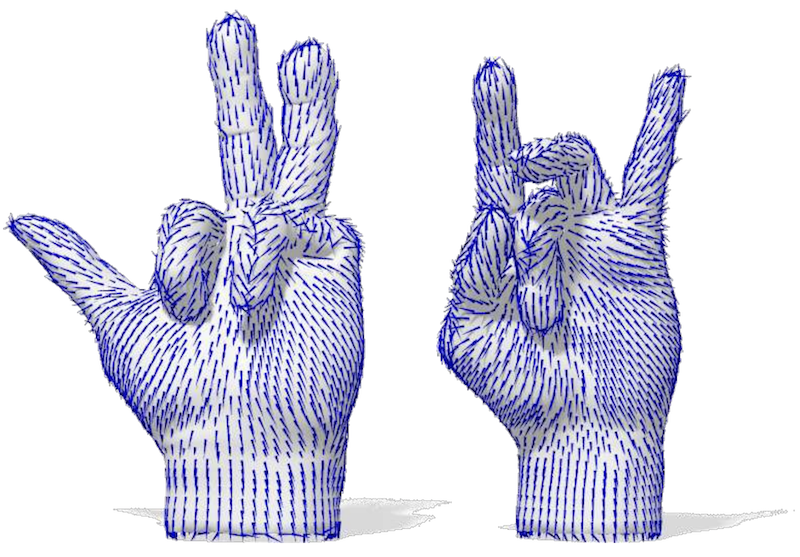
\includegraphics[width=1\linewidth]{figures/gframes.png} 
Example of stable gauges constructed on nearly-isometric manifolds (only one axis is shown) using the GFrames algorithm of \cite{melzi2019gframes}.
} 
%(such as e.g. the North and South pole of the sphere in the sidebar), for instance taking the two frame vectors to correspond to the highest and least curved direction on a 2D manifold. 
%
Moreover, such constructions are stable, i.e., the frames constructed this way will be identical on isometric manifolds and similar on approximately isometric ones. 
%
Such approaches were in fact employed in the early works on deep learning on manifolds  \citep{masci2015geodesic,monti2017geometric}.
%the same frame is found for isometric manifolds, and for nearly isometric ones a similar frame is found. 


Nevertheless, this solution is not entirely satisfactory because near singularities, the filter orientation (being defined in a fixed manner relative to the gauge) will vary wildly, leading to a non-smooth feature map even if the input signal and filter are smooth. 
%
Moreover, there is no clear reason why a given direction at some point $u$ should be considered equivalent to another direction at an altogether different point $v$. 
%
Thus, despite {\em practical} alternatives, we will look next for 
%methods based on semi-intrinsic frames can be useful, 
a more {\em theoretically} well-founded approach that would be altogether independent on the choice of gauge. 
%which we will discuss next. 
%We will discuss just such an approach next.


%\joan{This is still a bit long, but already much improved from earlier versions. 
%One aspect that is still not very explicit is how to precisely connect with the GDL blueprint, in terms of the composition of local equivariant maps, and global invariant map. 
%Here we argue that differential operators such as the Laplacian are defined intrinsically (isometry invariant), and thus any representation that is based on it will preserve this isometric invariance. Equivariance in this context is less obvious (equivariance with respect to changes in the gauge, parametrisation/charting?).

%Also, should we mention stability of the Laplacian to metric deformations? How to ensure that the information we extract from the Laplacian is not too unstable? we can mimic the discussion from previous section on wavelet vs fourier, to illustrate that the high-frequency eigenfunctions of the laplace-beltrami  are unstable. THis is mentioned in the mesh section, should it be restated here as well?
%}

%
%
%Assume now we have some vector-valued data $\Omega$. 
%In differential geometry, this is modelled as a {\em vector field} $x:\Omega \rightarrow T\Omega$, assigning to each point $u \in \Omega$ a tangent vector $x(u) \in T_u \Omega$. 
%%
%%
%%The reason we need to consider gauges is that we can only describe geometric data numerically \emph{relative to a gauge}.
%%
%Relative to a gauge, we can express each tangent vector as a coordinate vector, i.e. an array of numbers, and so a vector field becomes a map $\mathbf{x} : \Omega \rightarrow \R^{s}$.
%%
%In other words, we can, as previously, think of vector fields as signals forming the space $\mathcal{X}_{\R^s}(\Omega)$ with the inner product 
%%(\ref{eqn:innerprod}) [Only well defined if we choose a metric? Should we assume Riemannian manifolds?]. 
%$$
%\langle x, y\rangle = 
%\int_\Omega  \langle x(u), y(u) \rangle_{T_u\Omega} du = 
%\int_\Omega \mathbf{x}^\top(u) \mathbf{G}(u) \mathbf{y}(u) du,  
%$$
%%
%where $\mathbf{G}$ is the representation of the {\em Riemannian metric} (defined as an inner product on $T_u\Omega$ depending smoothly on $u$) in the same local frame.
%%

%As in the examples discussed in previous sections, this group can act via different representation $\rho$, which in this case corresponds to different kinds of fields, including scalar fields, vector fields, tensor fields, each of which is characterized by how it transforms under a change of gauge.



%\paragraph{Local Symmetries and Spatial Weight Sharing}


% ----
% OLD:

% Let us start from the simplest case of {\em scalar fields}, i.e. signals $\mathcal{X}(\Omega, \mathbb{R})$. 
% %




% Importantly, not only the {\em features} change when we change the gauge, also the {\em network layers} depend on the choice of gauge. 
% %
% Consider an architecture in the spirit of `message passing' we saw in graph neural networks, where at each point $u\in \Omega$, we aggregate the transformed feature vectors from neighbor points $v$, 
% and 
% %
% for simplicity, assume this transformation is linear. 
% %
% When the vectors are expressed w.r.t. a gauge, this transformation takes the form of matrix multiplication  $\mathbf{A}(u,v)\mathbf{x}(v)$; this notation emphasizes the fact that the matrix can be different for each pair of points $u, v$.  
% %.\marginnote{What we describe here is the GCN architecture. In attentional architectures, we can have $\mathbf{A}(\mathbf{x}(u),\mathbf{x}(u'))$ rather than $\mathbf{A}(u, u')$. }
% %
% %Note however an crucial difference: on a graph, the matrix $\mathbf{A}$ must be {\em the same} for all points $u'$, as this is needed for permutation equivariance. 
% %
% %In the case of a manifold, there is no such a global symmetry, so we can use a different matrix $\mathbf{A}(u,u')$ for each pair of (neighbor) points. 



% If we perform a gauge transformation, the input feature vector changes as $\mathbf{x}(u) \mapsto \rho(\fg(u)) \mathbf{x}(u)$, and the output feature should change as $\mathbf{x}(v) \mapsto \rho(\fg(v)) \mathbf{x}(v)$\marginnote{We assume here for simplicity that the input and output features are of the same type and thus have the same representation $\rho(\fG)$.}.
% It follows that we should change $\mathbf{A}(u,v) \mapsto \rho(\fg(v)) \mathbf{A}(u,v) \rho(\fg(u))^{-1}$.
% Although the new weight matrix and feature vectors contain different numbers, the underlying geometric objects are mapped in the same way regardless of the gauge.



% % Gauge equivariant message; 
% If gauge transformations are considered as symmetries, a network layer, and hence an individual message, should be equivariant to gauge transformations.
% That is, the weight matrix $A_{uu'}$ should satisfy $\rho(g(u'))^{-1} A_{uu'} = A_{uu'} \rho(g(u))$ for all gauge transformations $g : \Omega \rightarrow \fG$.
% This is an extremely strong constraint, because $g(u)$ and $g(u')$ (the gauge transformation at $u$ and $u'$) can vary independently.
% As a consequence the weight matrix $A_{uu'}$ is so constrained that it cannot learn very interesting mappings.

% % Connection
% The solution is to introduce an additional piece of structure called a \emph{connection}, which relates the feature spaces at $u$ and $u'$. % via parallel transport (see Figure TODO).
% The connection gives us for any two nearby points $u, u'$ a straightest curve (geodesic) between them, and a notion of \emph{parallel transport} of frames and feature vectors along this curve (see Figure TODO).
% %The parallel transporter from $u$ to $u'$ along a geodesic is an element of $\fG$ denoted $\fg_{u \rightarrow u'} \in \fG$ that transforms as $\fg_{u \rightarrow u'} \mapsto \fg(u') \fg_{u \rightarrow u'} \fg(u)^{-1}$ under a gauge transformation $\fg(u)$.
% Using parallel transport, we can move the feature vector $v_u$ at $u$ to $u'$, before applying the weight matrix $A_{uu'}$.
% Since this matrix maps input features at $u$ to output features at $u$, it only has to deal with the gauge at $u$.
% In other words, it should satisfy a more conventional equivariance constraint: $A_{uu'} \rho(g(u)) = \rho(g(u)) A_{uu'}$ that only involves $g(u)$ and not $g(u')$. \michael{[TACO: isn't it the other way around, you transport vectors from u' to u?]}

% % Spatial weight sharing; filter on tangent plane; identify tangent planes via gauge;
% What we have seen so far is that gauge symmetries constrain the weight matrix $A_{uu'}$, but that the weight matrices associated with different points need not necessarily share weights as in a convolution layer.




%In each of the examples discussed so far, we started with a space $\Omega$ and a group of symmetries $\fG$ acting on it.
%In some cases however, e.g. when the domain $\Omega$ is a general manifold or mesh, it may not have any obvious symmetries.
%%For instance, if $\Omega$ is a general manifold, it may not have any non-trivial symmetries.
%In this case, we cannot define an action of $\fG$ on the space of signals on $\Omega$ and use it to slide filters around to define a convolution.
%Nevertheless, in this example as many others, there is still a group of symmetries lurking beneath the surface, but this is an altogether kind of symmetry known as \emph{gauge symmetry}.
%
%The word gauge here refers to a choice of frame (ordered basis) for a vector space, or more generally to one such choice for each vector space in a collection of vector spaces $V_u$ associated with the points $u \in \Omega$.
%For example, if we have a manifold $\Omega$, we can construct the \emph{tangent bundle} $T \Omega$ which consists of a collection of vector spaces $T_u \Omega$ (the tangent spaces), one for each point in $u \in \Omega$ (see Figure TODO).
%So in this example a gauge is a choice of frame for each of the tangent spaces $T_u \Omega$.\marginnote{
%We note that in mathematical gauge theory one would require the gauge to be smooth, in which case a globally defined gauge may not always exist. We will ignore these subtleties and not insist on smoothness.
%}
%
%The reason we need to consider gauges is that we can only describe geometric data numerically \emph{relative to a gauge}.
%Let's imagine our data consists of a vector field on $\Omega$.
%A vector field assigns to each point $u \in \Omega$ a tangent vector $v \in T_u \Omega$.
%Relative to a gauge, we can express each tangent vector as a coordinate vector, i.e. a list of numbers, and so a vector field becomes a map $x : \Omega \rightarrow \R^{n}$ (where $n$ is the dimension of the manifold and tangent spaces).
%In other words, our input space is $\mathcal{X}(\Omega, \R^n)$.
%However it is important to realize that what we are really interested in is the underlying geometrical object (vector field), whose representation as a function $x \in \mathcal{X}(\Omega, \R^n)$ depends on the choice of gauge.
%%However there is no canonical choice of gauge, so depending on our choice we will get different coordinate vectors.
%
%When we change the gauge, there is at each position a unique invertible matrix that maps the old gauge to the new one.
%In other words, a gauge transformation is a mapping $g : \Omega \rightarrow \GL{n}$, where $\GL{n}$ is the group of invertible $n \times n$ matrices.
%We can also restrict our attention to e.g. right-handed orthogonal frames, which are related by rotations, in which case a gauge transformation is a map $g : \Omega \rightarrow \SO{n}$ assigning to each position a rotation.
%In general, one considers a group $\fG$ (called the structure group) and a collection of frames such that for any two of them there is a unique $\fg \in \fG$ that maps one frame onto the other.
%As in the examples discussed in previous sections, this group can act via different representation $\rho$, which in this case corresponds to different kinds of fields, including scalar fields, vector fields, tensor fields, each of which is characterized by how it transforms under a change of gauge.
%
%% Associated bundles / reps of G
%% In the previous sections on Graphs, Grids and Groups, we discussed how the same group may act on various feature spaces through different representations $\rho$.
%% In the case of gauge transformations the same is true: we can define various kinds of fields such as scalar, vector, and tensor fields, by choosing an appropriate representation $\rho$ of the structure group $\fG$.
%% For instance, a scalar field (e.g. surface temperature on earth) does not depend on the frame (a scalar does not have a direction), so it corresponds to the trivial representation $\rho_0(g) = 1$.
%% A 2-tensor field would transform as $A_u \mapsto \fg A_u \fg^T$, where $u \in \Omega$, $A_u \in \R^{n \times n}$ and $\fg \in \fG$ is the change of basis matrix relating two gauges.
%
%%Given two vector fields, we can take at each position the outer (tensor) product $v w^T$ to obtain a tensor field, which tra
%
%% Gauge equivariant message from u to v; need for a connection / parallel transport
%%If gauge transformations are considered as symmetries, a network layer should be equivariant to gauge transformations.
%Not only the features change when we change the gauge, also the network layers depend on the choice of gauge.
%We will consider a message passing layer, and focus first on a single message sent from $u \in \Omega$ to $u' \in \Omega$.
%In a graph neural network, one would take the feature vector $v_u$ at $u$ and multiply it by a weight matrix $A$ to get the feature vector $v_{u'}$ at $u'$, before summing over all neighbours $u'$.
%The same weight matrix is used for all pairs of adjacent points $u,u'$, because this is required for equivariance to permutations.
%In the case of a manifold, we don't have such a global symmetry, so we are free to use a different matrix $A_{uu'}$ for each pair of (nearby) points $u, u'$.
%Now if we perform a gauge transformation, the input feature changes as $v_u \mapsto \rho(g(u)) v_u$, and the output feature should change as $v_{u'} \mapsto \rho(g(u')) v_{u'}$\marginnote{We assume here that the input and output feature are of the same type, i.e. have the same representation $\rho$ of $\fG$.}.
%It follows that we should change $A_{uu'} \mapsto \rho(g(u')) A_{uu'} \rho(g(u))^{-1}$.
%Although the new weight matrix and feature vectors contain different numbers, the underlying geometric objects are mapped in the same way regardless of the gauge.
%
%% Gauge symmetries / gauge equivariance
%To say that gauge transformations are symmetries is to say that any two gauges related by a gauge transformation are to be considered equivalent. %, and that data expressed relative to these frames should be processed in the same way regardless of the gauge.
%For instance, if we take $\fG = \SO{n}$, any two right-handed orthogonal frames are considered equivalent, because we can map any such frame to any other such frame.
%In other words, there is are no distinguished local directions such as ``up'' or ``right''.
%Similarly, if $\fG = \Orth{n}$, then any left and right handed orthogonal frame are considered equivalent.
%In this case, there is no preferred orientation either.
%
%% Gauge equivariant message; 
%If gauge transformations are considered as symmetries, a network layer, and hence an individual message, should be equivariant to gauge transformations.
%That is, the weight matrix $A_{uu'}$ should satisfy $\rho(g(u'))^{-1} A_{uu'} = A_{uu'} \rho(g(u))$ for all gauge transformations $g : \Omega \rightarrow \fG$.
%This is an extremely strong constraint, because $g(u)$ and $g(u')$ (the gauge transformation at $u$ and $u'$) can vary independently.
%As a consequence the weight matrix $A_{uu'}$ is so constrained that it cannot learn very interesting mappings.
%
%% Connection
%The solution is to introduce an additional piece of structure called a \emph{connection}, which relates the feature spaces at $u$ and $u'$. % via parallel transport (see Figure TODO).
%The connection gives us for any two nearby points $u, u'$ a straightest curve (geodesic) between them, and a notion of \emph{parallel transport} of frames and feature vectors along this curve (see Figure TODO).
%%The parallel transporter from $u$ to $u'$ along a geodesic is an element of $\fG$ denoted $\fg_{u \rightarrow u'} \in \fG$ that transforms as $\fg_{u \rightarrow u'} \mapsto \fg(u') \fg_{u \rightarrow u'} \fg(u)^{-1}$ under a gauge transformation $\fg(u)$.
%Using parallel transport, we can move the feature vector $v_u$ at $u$ to $u'$, before applying the weight matrix $A_{uu'}$.
%Since this matrix maps input features at $u$ to output features at $u$, it only has to deal with the gauge at $u$.
%In other words, it should satisfy a more conventional equivariance constraint: $A_{uu'} \rho(g(u)) = \rho(g(u)) A_{uu'}$ that only involves $g(u)$ and not $g(u')$.
%
%% Spatial weight sharing; filter on tangent plane; identify tangent planes via gauge;
%What we have seen so far is that gauge symmetries constrain the weight matrix $A_{uu'}$, but that the weight matrices associated with different points need not necessarily share weights as in a convolution layer.
%
%----
%
%% Spatial weight sharing; filter on tangent plane; identify tangent planes via gauge;
%What we have seen so far is that gauge symmetries constrain the weight matrix $A_{uu'}$, but that the weight matrices associated with different points need not necessarily share weights as in a convolution layer.
%In order to share weights across spatial locations, we need to somehow identify local patches around each point in $\Omega$.
%A popular approach is based on the observation that these local patches can first be identified with the tangent planes $T_u \Omega$ via the exponential map (see Figure TODO). %, so that we can write $A_{uu'}$ instead as $A_{uv}$ where $v \in T_u \Omega$ is a tangent vector that satisfies $u' = \exp_u(v)$.
%Furthermore, the tangent spaces themselves can be identified with $\R^n$ through the choice of a gauge.
%Hence, we can define the filter as a matrix-valued function $A$ on $\R^n$ (which parameterizes the neighbour $u'$) and which is independent of $u$.
%
%Since the filter is now tied to the gauge, it will be rotated when we rotate the gauge.
%Hence, the equivariance constraint becomes $A(g v) = \rho(g) A(v) \rho(g)^{-1}$.
%
%Thus, we can define a gauge equivariant convolution of a field $x$ on $\Omega$ and a filter $A$ as follows:
%\begin{equation}
%    (x \star A)(u) = \int_{\R^n} A(v) \, \rho(\fg_{\exp_u(v) \rightarrow u}) \, x(\exp_u(v)) dv,
%\end{equation}
%where $\exp_u(v)$ denotes the neighbour $u'$ indexed by $v \in \R$ and $\fg_{\exp_u(v) \rightarrow u} \in \fG$ denotes the parallel transport from this neighbour to $u$.
%



%---


% If gauge transformations are considered as symmetries, a mapping (network layer) $f : \mathcal{X}(\Omega, \R^n) \rightarrow \mathcal{X}(\Omega, \R^m)$ should be equivariant to gauge transformations.
% As a first example, consider a $1 \times 1$ convolution, i.e. $f$ consists of applying a linear map $\psi : \R^n \rightarrow \R^m$ at each position $u \in \Omega$.
% The input feature vector $v_u \in \R^n$ is a coordinate vector defined relative to some choice of gauge, and we will want that the output feature vector $w_u = \psi(v_u)$ is expressed relative to the same gauge.
% If we change the gauge by $g_u \in \fG$, then the input transforms as $v_u \mapsto \rho_{\textup{in}}(g_u) v_u$ and the output should transform by $w_u \mapsto \rho_{\textup{out}}(g_u) w_u$.
% Hence we $\psi$ should be equivariant: $\psi \circ \rho_{\textup{in}}(g_u) = \rho_{\textup{out}}(g_u) \circ \psi$ for all $g_u \in \fG$.

% The example of a $1 \times 1$ convolution is simple, because the input and output feature vectors $v_u$ and $w_u$ have the same spatial position $u \in \Omega$, and hence are represented with respect to the same gauge.
% In a general convolution, one would sum/integrate the messages sent from points $u'$ near $u$ as well, using a learned map $\psi_{uu'} : \R^n \rightarrow \R^m$.
% For this function we would have the constraint $\psi_{uu'} \circ \rho_{\textup{in}}(g_{u'}) = \rho_{\out}(g_u) \circ \psi_{uu'}$.
% However, since $g_u$ and $g_{u'}$ can vary independently (we can freely change the gauge at each position separately), this is an overly constraint and any $\psi_{uu'}$ that satisfies it will be uninteresting.

% The remedy is to introduce an object called a \emph{connection} that tells us how to compare feature vectors at $u$ and feature vectors at $u'$.
% That is, we take a map $c_{u \rightarrow u'} : \R^n \rightarrow \R^n$ 
% [TBC...]

%[Discuss internal symmetries.]

% In the context of geometric deep learning, the vector space in question is $\mathcal{C}$, i.e. the feature vector space that is attached to each position in $\Omega$ to build the space $\mathcal{X}(\Omega, \mathcal{C})$ of signals $x : \Omega \rightarrow \mathcal{C}$.


% The word gauge here refers to a choice of frame (ordered basis) for a vector space.
% In the context of geometric deep learning, the vector space in question is $\mathcal{C}$, i.e. the feature vector space that is attached to each position in $\Omega$ to build the space $\mathcal{X}(\Omega, \mathcal{C})$ of signals $x : \Omega \rightarrow \mathcal{C}$.
% Consider for now just a single copy of $\mathcal{C}$.
% We know from linear algebra that a linear map $f : \mathcal{C} \rightarrow \mathcal{C}$ can be expressed as a matrix $A$ if we choose a frame for $\mathcal{C}$, and likewise a vector $V \in \mathcal{C}$ can be represented as a coordinate vector $v \in \R^n$.
% If we change the frame, the matrix representation of $f$ changes as $A \mapsto P A P^{-1}$, where $P$ is called the change of basis matrix in linear algebra, or gauge transformation, in physics.
% The coordinate vector changes as $v \mapsto P v$.

% If we consider $P$ as a gauge \emph{symmetry}, then $A$ should be equivariant, i.e. $PA = AP$.
% Equivalently, we should have $A = PAP^{-1}$, i.e. $A$ has the same matrix representation in all frames related by a gauge symmetry.
% Hence, the matrix $A$ can be applied to coordinate vectors not just in one frame, but also to any other frame related by a gauge symmetry.
% For instance, if we consider the group of rotations as gauge symmetries, then any two orthogonal frames of the same handedness can be considered equivalent and $A$ can be applied to coordinate vectors in any such frame.
% Similarly, if we consider both rotations and reflections to be gauge symmetries, the same is true for orthogonal frames of different handedness.

% In gauge theory, this idea is generalized in two ways.
% Firstly, since we are dealing with signals $x : \Omega \rightarrow \mathcal{C}$, we have not just one vector space $\mathcal{C}$, but one copy of $\mathcal{C}$ associated with every point $u \in \Omega$.\marginnote{The vector space attached at $u \in \Omega$ is sometimes called the fibre $\mathcal{C}_u$ at $u$.}
% We are free to choose a different basis for each of these vector spaces, and so a general gauge transformation consists of one transformation at each point in $\Omega$.
% In other words, a gauge transformation is a function $g : \Omega \rightarrow \fG$, where $\fG$ is called the structure group (e.g. rotations or roto-reflections in the examples above).

% Secondly, as in the case of global symmetries acting on $\Omega$, one may consider different representations $\rho$ of the same group $\fG$ in each feature space in the network.
% Thus, if we have a representation $\rho$ of $\fG$ in $\mathcal{C}$, then a gauge transformation $g : \Omega \rightarrow \fG$ acts on a signal $x : \Omega \rightarrow \mathcal{C}$ as $x(u) \mapsto \rho(g(u)) x(u)$.  % todo check if we need an inverse on g?

% \taco{TODO: work on formatting of examples}
% \begin{tcolorbox}[width=\linewidth,
%                   boxsep=0pt,
%                   left=7.5pt,
%                   right=7.5pt,
%                   top=7.5pt,
%                   bottom=7.5pt,
%                   arc=0pt,
%                   boxrule=0pt,toprule=0pt,
%                   colback=boxgray,
%                   ]%%
%     Example: tangent vectors on a manifold.
    
%     Consider a smooth manifold $\Omega$ of dimension $2$.
%     % For instance, $\Omega$ could be an iso-energy surface of a protein [cite Michael's paper].
%     At each point $u \in \Omega$, there is a tangent space $T_u \Omega$ (see Figure TODO).
%     A \emph{vector field} is an assignment of a vector $v_u \in T_u \Omega$ to each point $u \in \Omega$.
%     If we choose a frame for each tangent space, we can express a vector field as a function $v : \Omega \rightarrow \R^2$.
%     ...
% \end{tcolorbox}


% \begin{tcolorbox}[width=\linewidth,
%                   boxsep=0pt,
%                   left=7.5pt,
%                   right=7.5pt,
%                   top=7.5pt,
%                   bottom=7.5pt,
%                   arc=0pt,
%                   boxrule=0pt,toprule=0pt,
%                   colback=boxgray,
%                   ]%%
%     Example: color space symmetry.
    
    
% \end{tcolorbox}


%Typically a problem comes with a fixed structure group $\fG$ and space $\Omega$, but the feature spaces $\mathcal{X}(\Omega, \mathcal{C}_l)$ at each layer $l$ may 

% the matrix $A$ can be applied to coordinate vectors in any equivalent basis; if $w = Av$ and we change the basis, $v' = P v$ then $w' = A P v = P A v = P w$.
% That is, if we apply $A$ to a coordinate vector relative some basis, we get an output coordinate vector relative to the same basis.



% To postulate a gauge symmetry is to postulate that frames related by certain kinds of gauge transformations are equivalent.
% For instance, two frames related by a rotation or reflection, can be considered equivalent.
% Or if we care about handedness, only those frames related by a rotation should be considered equivalent.



% Both global symmetries acting on $\Omega$ and gauge symmetries acting on $\mathcal{C}$ change how a signal is represented numerically, e.g. in computer memory.
% However, whereas global symmetries considered act on the domain $\Omega$, gauge symmetries act on the range $\mathcal{C}$ of signals $x : \Omega \rightarrow \mathcal{C}$.
% For example, in the case of graphs, a permutation will shuffle the node feature vectors but not change the feature vectors themselves.
% Conversely, a gauge transformation will change the feature vectors but not move them around on $\Omega$.


\subsection{Gauges and Bundles}
\label{sec:gauges}

The notion of gauge, which we have defined as a frame for the tangent space, is 
%In the previous section we have already touched on the concept %of a gauge, defining it as a frame for the tangent space. 
%
%The notion of gauge as used in physics is however 
quite a bit more general in physics:  it can refer to a frame for any\marginnote{Historically, fibre bundles arose first in modern differential geometry of {\'E}lie Cartan (who however did not define them explicitly), and were then further developed as a standalone object in the field of topology in the 1930s.} \emph{vector bundle}, not just the tangent bundle. 
%
Informally, a vector bundle describes a family of vector spaces parametrised by another space and 
consists of a \emph{base space} $\Omega$ with an identical vector space $\mathbb{V}$ (called the \emph{fibre}) attached to each position $u \in \Omega$ (for the tangent bundle these are the tangent spaces $T_u\Omega$).  
%and a continuous {\em projection function} $\pi : V \rightarrow \Omega$. 
%
Roughly speaking, a bundle looks as a product $\Omega \times \mathbb{V}$ locally around $u$, but globally might be `twisted' and have an overall different structure. 
%
%A {\em section} of the bundle is a 
%collection of identical vector spaces attached to the points in the manifold $\Omega$. 
%
%
%
%
In Geometric Deep Learning, fibres %in question are 
can be used to model the feature spaces at each point in the manifold $\Omega$, with the dimension of the fibre being equal to the number of feature channels. 
In this context, a new and fascinating kind of symmetry, called \emph{gauge symmetry} may present itself.% \joan{Good opening. Can we give a concrete example of this symmetry? Physics application?}

%[Say something about setting? Assume manifold is known and the same for all data points. Each data point is a different signal on it. This is different from previous section where we assume manifold is different for each data point / manifold is part of the data.]


%\joan{Mobius strip}

%\joan{Field theory invariants -- ask Kyle for a nice example}
%Before we discuss the general case, 


Let us consider again an $s$-dimensional manifold $\Omega$ with its tangent bundle $T\Omega$, and a vector field 
%consider again a vector field 
$X : \Omega \rightarrow T \Omega$ (which in this terminology is referred to as a {\em section} on the tangent bundle). 
%
Relative to a gauge $\omega$ for the tangent bundle, $X$ is represented as a function $\mathbf{x} : \Omega \rightarrow \R^s$.
However it is important to realise that what we are really interested in is the underlying geometrical object (vector field), whose representation as a function $\mathbf{x} \in \mathcal{X}(\Omega,\R^s)$ {\em depends on the choice of gauge} $\omega$. 
%
If we change the gauge, we also need to change $\mathbf{x}$ so as to preserve the underlying vector field being represented.

%\michael{Give a comment from physics where this need arises: general relativity?}

%Likewise, we then need to change the layers of the network so that when they receive inputs expressed relative to the new gauge, they also produce outputs relative to that gauge; like a change of basis, but for many vector spaces at once.

% Taco: note, this itself is not gauge equivariance yet. Only if we *dont* need to change the map, yet it passes through gauge transformations, we have gauge equivariance.
%Since there is no `canonical' way to set a gauge, 
%we must ensure $x$ transforms appropriately when the gauge is changed -- a property we will call {\em gauge-equivariance}. 

%
%\begin{figure}[h!]
%    \centering
%    %\includegraphics{}
%    \caption{TODO: figure showing a manifold with a vector field on it, with one tangent plane drawn. In this tangent plane, a frame is drawn. The coordinates of the vector on that tangent plane is shown below. On the right, an identical figure but with a different frame, and different coordinates. Alternatively, we can draw a plane with a vector field on it. Then we dont draw tangent planes but we draw frames at regularly spaced intervals. The vector field is the same for the left and right figure, but the frame is different.}
%    \label{fig:into:vector-field-gauge}
%\end{figure}


%However there is no canonical choice of gauge, so depending on our choice we will get different coordinate vectors.

%\joan{Here we could already give a couple of examples. 
%
%}


\paragraph{Tangent bundles and the Structure group}
When we change the gauge, we need to apply at each point an   invertible matrix that maps the old gauge to the new one.  This matrix is unique for every pair of gauges at each point, but possibly different at different points.  
%
%\marginnote{We can also restrict our attention to e.g. right-handed orthogonal frames, which are related by rotations, in which case a gauge transformation is a map $\fg : \Omega \rightarrow \SO{s}$ assigning to each position a rotation.} 
In other words, a {\em gauge transformation} is a mapping $\fg : \Omega \rightarrow \GL{s}$, where $\GL{s}$ is the {\em general linear group} of invertible $s \times s$ matrices.
It acts on the gauge $\omega_u : \R^s \rightarrow T_u \Omega$ to produce a new gauge $\omega'_u = \omega_u \circ \fg_u : \R^s \rightarrow T_u \Omega$. 
%
The gauge transformation acts on a coordinate vector field %$\mathbf{x}$
at each point 
via $\mathbf{x}'(u) = \fg^{-1}_u \mathbf{x}(u)$ to produce the coordinate representation $\mathbf{x}'$ of $X$ relative to the new gauge.
%
The underlying vector field remains unchanged: 
$$
X(u) = \omega'_u(\mathbf{x'}(u)) = \omega_u( \fg_u \fg^{-1}_u \mathbf{x}(u)) = \omega_u(\mathbf{x}(u)) = X(u), 
$$
which is exactly the property we desired. 
%
%
%
More generally, we may have a field of geometric quantities that transform according to a representation $\rho$ of $\GL{s}$, e.g. a field of 2-tensors (matrices) $\mathbf{A}(u) \in \R^{s \times s}$ that transform like $\mathbf{A'}(u) = \rho_2(\fg^{-1}_u) \mathbf{A}(u) = \rho_1(\fg_u) \mathbf{A}(u) \rho_1(\fg^{-1}_u)$. %\michael{The notation here is confusing: before we had $\rho$ as a matrix acting on vectors. Here it acts on both sides of $A$. Perhaps we should already mention the same thing when talking about graphs, where we have the representation of permutations acting on the adjacency matrix? }
%\taco{Decision: use $\mathbf{R}$ as the matrix representation of $\fg$}
In this case, the gauge transformation $\fg_u$ acts via $\rho(\fg_u)$.

Sometimes we may wish to restrict attention to frames with a certain property, such as orthogonal frames, right-handed frames, etc.
Unsurprisingly, we are interested in a set of  some property-preserving transformations that  form a group.
For instance, the group that preserves orthogonality is the orthogonal group $\Orth{s}$ (rotations and reflections), and the group that additionally preserves  orientation or `handedness' is $\SO{s}$ (pure rotations).
Thus, in general we have a group $\fG$ called the \emph{structure group} of the bundle, and a gauge transformation is a map $\fg : \Omega \rightarrow \fG$.
A key observation is that in all cases with the given property, for any two frames at a given point there exists exactly one gauge transformation relating them.

%\taco{Introduce parallel transport here? Say it is $\fG$-valued}

As mentioned before, gauge theory extends beyond tangent bundles, and in general, we can consider a bundle of vector spaces whose structure and dimensions are not necessarily related to those of the base space $\Omega$. \marginnote{We use $s$ to denote the dimension of the base space $\Omega$ and $d$ referring to the dimension of the fibre. For tangent bundles, $d=s$ is the dimension of the underlying manifold. For RGB image, $s=2$ and $d=3$.} 
For instance, a color image pixel has a position $u \in \Omega = \Z^2$ on a 2D grid and a value $\mathbf{x}(u) \in \R^3$ in the RGB space, so the space of pixels can be viewed as a vector bundle with base space $\Z^2$ and a fibre $\R^3$ attached at each point. 
%
It is customary to express an RGB image relative to a gauge that has basis vectors for R, G, and B (in that order), so that the coordinate representation of the image looks like $\mathbf{x}(u) = (r(u), g(u), b(u))^\top$.
But we may equally well permute the basis vectors (color channels) independently at each position, as long as we remember the frame (order of channels) in use at each point\marginnote{In this example we have chosen $\fG = \Sigma_3$ the permutations of the 3 color channels as the structure group of the bundle. Other choices, such as a Hue rotation $\fG = \SO{2}$ are also possible.}.
As a computational operation this is rather pointless, but as we will see shortly it is conceptually useful to think about gauge transformations for the space of RGB colors, because it allows us to express a gauge symmetry -- in this case, an equivalence between colors -- and make functions defined on images respect this symmetry (treating each color equivalently). 




As in the case of a vector field on a manifold, an RGB gauge transformation changes the numerical representation of an image (permuting the RGB values independently at each pixel) but not the underlying image. 
%
In machine learning applications, we are interested in constructing functions $f \in \mathcal{F}(\mathcal{X}(\Omega))$ on such images (e.g. to perform image classification or segmentation), implemented as layers of a neural network. 
%
It follows that if, for whatever reason, we were to apply a gauge transformation to our image, we would need to also change the  function $f$ (network layers) so as to preserve their meaning. 
Consider for simplicity a $1 \times 1$ convolution, i.e. a map that takes an RGB pixel $\mathbf{x}(u) \in \R^3$ to a feature vector $\mathbf{y}(u) \in \R^C$.
According to our Geometric Deep Learning blueprint, the output is associated with a group representation $\rho_{\textup{out}}$, in this case a $C$-dimensional representation of the structure group $\fG = \Sigma_3$ (RGB channel permutations), and similarly the input is associated with a representation $\rho_{\textup{in}}(\fg) = \fg$. %\michael{not clear: is $\fg$ a permutation here? You need to define how the C-dim representation of the permutation looks like}
Then, if we apply a gauge transformation to the input, we would need to change the linear map ($1 \times 1$ convolution) $f : \R^3 \rightarrow \R^C$ to $f' = \rho^{-1}_{\textup{out}}(\fg) \circ f \circ \rho_{\textup{in}}(\fg)$ so that the output feature vector $\mathbf{y}(u) = f(\mathbf{x}(u))$ transforms like $\mathbf{y}'(u) = \rho_{\textup{out}}(\fg_u) \mathbf{y}(u)$ at every point.
Indeed we verify: 
\begin{equation*}
    \mathbf{y}' = f'(\mathbf{x}') = \rho^{-1}_{\textup{out}}(\fg) f(\rho_{\textup{in}}(\fg) \rho^{-1}_{\textup{in}}(\fg) \mathbf{x}) = \rho^{-1}_{\textup{out}}(\fg) f(\mathbf{x}).\marginnote{Here the notation $\rho^{-1}(\fg)$ should be understood as the inverse of the group representation (matrix) $\rho(\fg)$.}
\end{equation*}

%\joan{Indeed, here I would illustrate these formulas in terms of their matrix representations. If $P_{\fg}$ is a $3x3$ permutation matrix and $F$ the linear (trainable) map expressed as a $C \times 3$ matrix, then we wish to characterise the matrices $Q_{\fg}$ indexed by the group $\Sigma_3$ so that
%$Q_{\fg}^{-1} F P_{\fg} $ does not depend on $\fg$, and thus 
%$Q_{\fg}^{-1} F P_{\fg} = F$ for all $\fg$?
%is this the main idea? }

%\michael{show an example! too abstract}

% Gauge symmetries / gauge equivariance
\paragraph{Gauge Symmetries}
To say that we consider gauge transformations to be symmetries is to say that any two gauges related by a gauge transformation are to be considered equivalent. %, and that data expressed relative to these frames should be processed in the same way regardless of the gauge.
For instance, if we take $\fG = \SO{d}$, any two right-handed orthogonal frames are considered equivalent, because we can map any such frame to any other such frame by a rotation.
In other words, there are no distinguished local directions such as ``up'' or ``right''.
Similarly, if $\fG = \Orth{d}$ (the orthogonal group), then any left and right handed orthogonal frame are considered equivalent.
In this case, there is no preferred orientation either.
%
%
%
In general, we can consider a group $\fG$ %  \marginnote{Such $\fG$ is called the {\em structure group} of the (tangent) bundle.}
and a collection of frames at every point $u$ such that for any two of them there is a unique $\fg(u) \in \fG$ that maps one frame onto the other. 
%

%\joan{Beware notation; is $d$ the right choice here?}

Regarding gauge transformations as symmetries in our Geometric Deep Learning blueprint, we are interested in making  
%network layers 
the functions $f$ acting on signals defined on $\Omega$ and expressed with respect to the gauge should equivariant to such transformation. 
%
Concretely, this means that if we apply a gauge transformation to the input, the output should undergo the same transformation (perhaps acting via a different representation of $\fG$).
We noted before that when we change the gauge, the function $f$ should be changed as well, but for a gauge equivariant map this is not the case: changing the gauge leaves the mapping invariant.
To see this, consider again the RGB color space example.
The map $f : \R^3 \rightarrow \R^C$ is equivariant if $f \circ \rho_{\textup{in}}(\fg) = \rho_{\textup{out}}(\fg) \circ f$, but in this case the gauge transformation applied to $f$ has no effect: $\rho_{\textup{out}}^{-1}(\fg) \circ f \circ \rho_{\textup{in}}(\fg) = f$.
In other words, the coordinate expression of a gauge equivariant map is independent of the gauge, in the same way that 
in the case of graph, we applied the same function 
%a graph neural network applies the same layers 
regardless of how the input nodes were permuted. 
However, unlike the case of graphs and other examples covered so far, gauge transformations act {\em not on} $\Omega$ but separately {\em on each of the feature vectors} $\mathbf{x}(u)$ by a transformation $\fg(u) \in \fG$ for each $u \in \Omega$.
%\joan{This paragraph is not very easy to understand. Have we defined a `Gauge equivariant map' before? I think indeed it is a good idea to relate this notion to the previously introduced equivariances in graphs and grids.  }
%\taco{This paragraph is my attempt at defining them informally (see ``concretely ...'').}

%Different signals defined on $\Omega$ (e.g. scalar fields, vector fields, tensor fields) are affected differently by the action of $\fG$, which acts on them through the corresponding representation $\rho$ of $\fG$.
%

Further considerations enter the picture when we look at filters on manifolds with a larger spatial support. 
%
Let us first consider an easy example %: a network layer that maps 
of a mapping $f : \mathcal{X}(\Omega, \mathbb{R}) \rightarrow \mathcal{X}(\Omega, \mathbb{R})$ from 
scalar fields to scalar fields on an $s$-dimensional manifold $\Omega$. 
Unlike vectors and other geometric quantities, scalars do not have an orientation, so a scalar field $x \in \mathcal{X}(\Omega, \R)$ is {\em invariant} to gauge transformations (it transforms according to the trivial representation $\rho(\fg) = 1$). 
%\joan{assuming unitary gauges I guess?}. \taco{If we define scalar as ``transforming according to the trivial rep'' then no: we can have GL structure group / general frames, and yet have invariant scalars. E.g. one might have a 2D tangent plane with general linear frames, but a function on $\Omega$ doesn't care if you rotate or scale the frame. On the other hand one could define a 1D geometric quantity that transforms by the determinant of the gauge transformation (det being a non-unitary 1D rep.) But I think this is not whats usually meant by scalar in physics.}
Hence, any linear map from scalar fields to scalar fields is {\em gauge equivariant} (or invariant, which is the same in this case). 
For example, we could write $f$ similarly to~(\ref{eqn:conv_spat}), as a convolution-like operation with a position-dependent filter $\theta : \Omega \times \Omega \rightarrow \R$, %\michael{defined this way it's not local. Nor that in the Euclidean filter the filter is required to be local - a circulant matrix can be full, this is just a design consideration. }
\begin{equation}
    \label{eq:intro:general-linear-map-scalar-fields}
    (x \star \theta)(u) = \int_{\Omega} \theta(u, v) x(v) \mathrm{d}v.  
\end{equation}
This implies that we have a potentially different filter $\theta_u = \theta(u, \cdot)$ at each point, i.e., no spatial weight sharing --- which gauge symmetry alone does not provide. 
%require spatial weight sharing, for it acts separately on each point in $\Omega$.


Consider now a more interesting case of a mapping $f : \mathcal{X}(\Omega, T\Omega) \rightarrow \mathcal{X}(\Omega, T\Omega)$ from vector fields to vector fields. 
%
Relative to a gauge, the input and output vector fields $X, Y \in \mathcal{X}(\Omega, T\Omega)$ are vector-valued functions $\mathbf{x}, \mathbf{y} \in \mathcal{X}(\Omega, \R^s)$. 
%
A general linear map between such functions can be written using the same equation we used for scalars  (\ref{eq:intro:general-linear-map-scalar-fields}), only replacing the scalar kernel by a matrix-valued one $\boldsymbol{\Theta} : \Omega \times \Omega \rightarrow \R^{s \times s}$.
%
The matrix $\boldsymbol{\Theta} (u, v)$ should map tangent vectors in $T_v\Omega$ to tangent vectors in $T_u\Omega$, but these points have {\em different gauges} that we may change {\em arbitrarily and independently.} 
%
 That is, the filter would have to satisfy $\boldsymbol{\Theta} (u, v) = \rho^{-1}(\fg(u)) \boldsymbol{\Theta}(u, v) \rho(\fg(v))$ for all $u, v \in \Omega$, where $\rho$ denotes the action of $\fG$ on vectors, given by an $s\times s$ rotation matrix. 
 %
Since $\fg(u)$ and $\fg(v)$ can be chosen freely, this is an overly strong constraint on the filter. \marginnote{Indeed $\boldsymbol{\Theta}$ would have to be zero in this case}
%\michael{Perhaps explain why: give a 2D example?}


A better approach is to first transport the vectors to a common tangent space by means of the connection,  and then impose gauge equivariance w.r.t. a single gauge transformation at one point only. 
%To obtain a non-trivial mapping between vector fields, we require a connection which allows us to parallel transport vectors between two tangent spaces. 
Instead of (\ref{eq:intro:general-linear-map-scalar-fields}), we can then define the following map between vector fields,
\begin{equation}
    (\mathbf{x} \star \boldsymbol{\Theta})(u) = \int_\Omega \boldsymbol{\Theta}(u, v) \rho(\fg_{v \rightarrow u}) \mathbf{x}(v) \mathrm{d}v,\label{eqn:gauge_eq_conv}
\end{equation}
where $\fg_{v \rightarrow u} \in \fG$ denotes the parallel transport from $v$ to $u$ along the geodesic connecting these two points;  
%
its representation $\rho(\fg_{v \rightarrow u})$ is an $s \times s$ rotation matrix rotating the vector as it moves between the points. 
%
Note that this geodesic is assumed to be unique, which is true only locally and thus the filter must have a local support. 
%
%
Under a gauge transformation $\fg_u$, this element transforms as $\fg_{u \rightarrow v} \mapsto \fg_u^{-1} \fg_{u \rightarrow v} \fg_v$, and the field itself transforms as $\mathbf{x}(v) \mapsto \rho(\fg_v) \mathbf{x}(v)$. 
If the filter commutes with the structure group representation  $\boldsymbol{\Theta}(u, v) \rho(\fg_u) = \rho(\fg_u) \boldsymbol{\Theta}(u, v)$, %the above map is gauge-equivariant.
equation~(\ref{eqn:gauge_eq_conv}) defines a {\em gauge-equivariant convolution}, which transforms as  
$$ 
(\mathbf{x}' \star \boldsymbol{\Theta})(u) = \rho^{-1}(\fg_u) (\mathbf{x} \star \boldsymbol{\Theta})(u). 
$$ 
under the aforementioned transformation. %substitutions, we find that

%, where $\mathbf{x}(u) = \rho(\fg_u)^{-1} \mathbf{x}$.
% \begin{equation}
%     \int_\Omega \psi(u, v) \rho(\fg_u^{-1} \fg_{v \rightarrow u} \fg_v) \rho(\fg_v) \mathbf{x}(v) dv
%     = 
%     \rho(\fg_u)^{-1} \int_\Omega \psi(u, v) \rho(\fg_{v \rightarrow u}) \mathbf{x}(v) dv
% \end{equation}


% [Mention spatial weight sharing: covered in models section. Maybe explain basic idea in words here.]

%\taco{TODO: say that rho of PT is a rotation matrix. +Figure?}



\subsection{Geometric graphs and Meshes}
\label{sec:meshes}

We will conclude our discussion of different geometric domains with {\em geometric graphs} (i.e., graphs that can be realised in some geometric space) and {\em meshes}. 
%
%
In our `5G' of geometric domains, meshes fall somewhere between graphs and manifolds: in many regards, they are similar to graphs, but their additional structure allows to also treat them similarly to continuous objects. 
%
For this reason, we do not consider meshes as a standalone object in our scheme, and in fact, will emphasise that many of the constructions we derive in this section for meshes are directly applicable to general graphs as well.   
%




As we already mentioned in Section~\ref{sec:manifolds}, two-dimensional manifolds (surfaces) are a common way of modelling 3D objects (or, better said, the boundary surfaces of such objects).  In computer graphics and vision applications, such surfaces are often discretised as {\em triangular meshes}, \marginnote{Triangular meshes are examples of topological structures known as {\em simplicial complexes}.} 
which can be roughly thought of as a piece-wise planar approximation of a surface obtained by gluing triangles together along their edges. 
%
Meshes are thus (undirected) {\em graphs with additional structure}: in addition to nodes and edges, a mesh 
$\mathcal{T} = (\mathcal{V},\mathcal{E}, \mathcal{F})$ 
also have ordered triplets of nodes forming {\em triangular faces} $\mathcal{F} =  \{ (u,v,q) : u,v,q \in \mathcal{V} \,\,\, \text{and} \,\,\, (u,v), (u,q), (q,v) \in  \mathcal{E}\}$; the order of the nodes defines the face {\em orientation}. \marginnote{
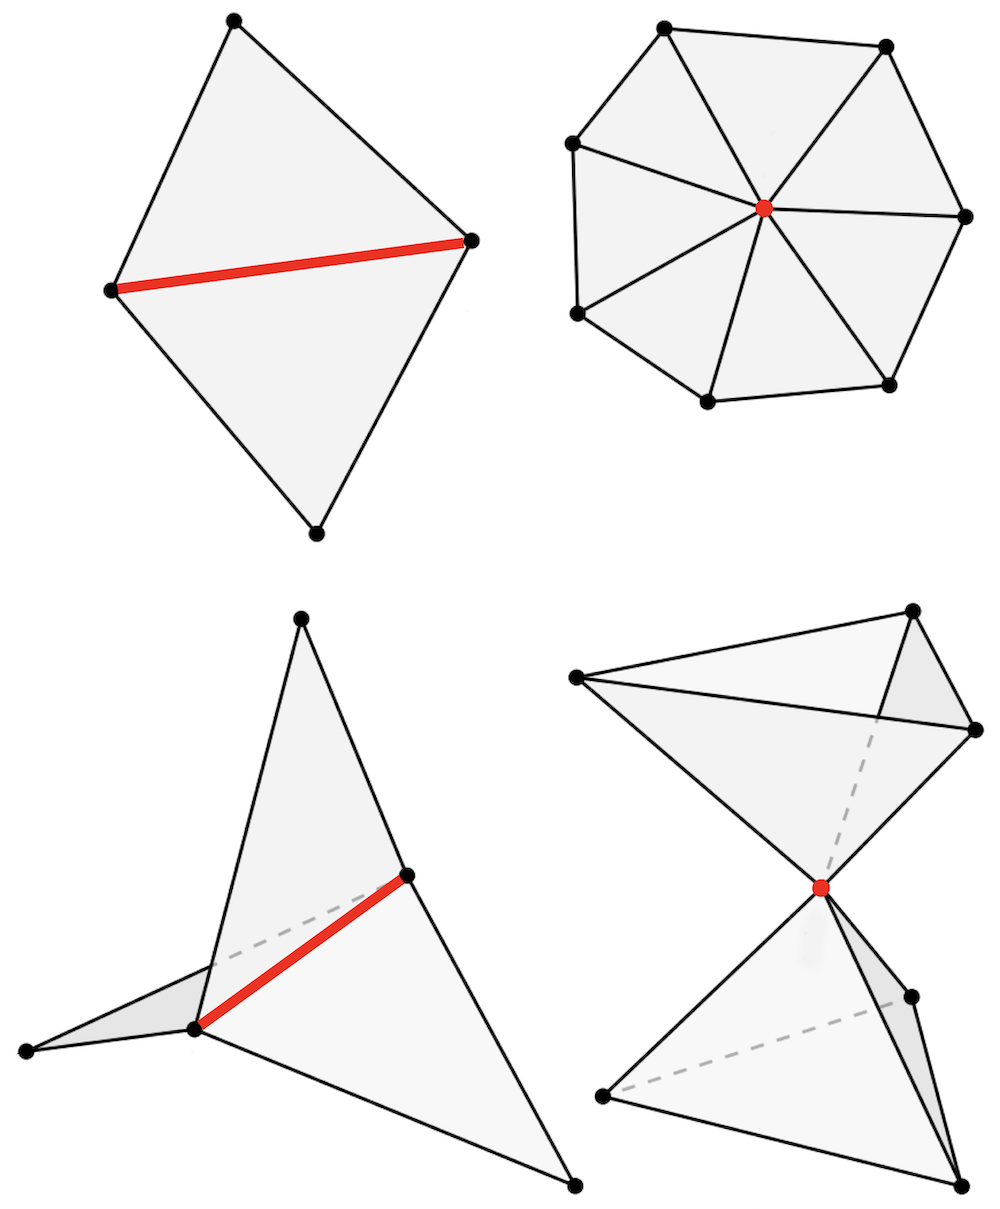
\includegraphics[width=0.9\linewidth]{figures/mesh.png}\\
%
Examples of manifold (top) and non-manifold (bottom) edges and nodes. 
For manifolds with boundary, one further defines {\em boundary edges} that belong to exactly one triangle. }
%
%We will denote meshes by $\mathcal{T} = (\mathcal{V},\mathcal{E}, \mathcal{F})$, where $\mathcal{F} =  \{ (i,j,k) : i,j,k \in \mathcal{V} \,\,\, \text{and} \,\,\, (i,j), (i,k), (k,j) \in  \mathcal{E}\}$ and use them as our domain $\Omega$.  


It is further assumed that that each edge is shared by exactly two triangles, and the boundary of all triangles incident on each node forms a single loop of edges. This condition guarantees that 1-hop neighbourhoods around each node are disk-like and the mesh thus constitutes a {\em discrete manifold} -- such meshes are referred to as {\em manifold meshes}. 
%In particular, 
%
%
%
Similarly to Riemannian manifolds, we can define a {\em metric} on the mesh. In the simplest instance, it can be  induced from the embedding of the mesh nodes $\mathbf{x}_1, \hdots, \mathbf{x}_n$ and expressed through the Euclidean length of the edges, $\ell_{uv} = \| \mathbf{x}_u - \mathbf{x}_v \|$. 
%
A metric defined in this way automatically satisfies properties such as the {\em triangle inequality}, i.e., expressions of the form 
$
\ell_{uv} \leq \ell_{uq} + \ell_{vq}
$
for any $(u,v,q) \in \mathcal{F}$ and any combination of edges. %
%
Any property that can be expressed solely in terms of $\ell$ is {\em intrinsic}, and any deformation of the mesh preserving $\ell$ is an {\em isometry}  -- these notions are already familiar to the reader from our discussion in Section~\ref{sec:manifolds}.   
%


%
%\paragraph{Mesh isometries and rigidity}
%Whether meshes have {\em non-trivial isometries} (i.e. embeddings that do not differ by only a rigid motion) is a deep question with fascinating history. %, and results here are starkly different from the continuous case. 
%%
%In 1766, Leonhard Euler conjectured that every polyhedron (a surface made of polygonal faces, on which a triangular mesh is a particular case) is {\em rigid}: that is, if one imagines a polyhedron as made of metal plates connected by hinges, it would not be possible to move them without bending. This assertion became known as the {\em Rigidity Conjecture} and gave birth to entire theory with the same name.  
%%
%\marginnote{
%\includegraphics[width=1\linewidth]{figures/connelly.png}\\
%%
%A convex polyhedron (icosahedron, left) is rigid by virtue of Cauchy's theorem. A non-convex polyhedron constructed by Klaus Steffen (right) is non-rigid and can be continuously deformed. 
%}
%%
%In 1813, Cauchy succeeded proving that every {\em convex} polyhedron is rigid in 3D \citep{cauchy1813recherche}. 
%%
%In 1897, a Belgian engineer and mathematician Raoul Bricard showed a construction of several flexible polyhedra \citep{bricard1897memoire}, which however, had self-intersections and thus could not be folded out of paper. 
%%
%In 1977, Robert Connelly showed  a non-rigid polyhedron without self-intersections (henceforth called the `Connelly Sphere') finally disproving Euler's conjecture by counter-example \citep{connelly1977counterexample}.  
%%
%A simpler (and in fact the simplest currently known) construction was shown a year later by the German geometry Klaus Steffen; his polyhedron can be easily folded of paper and bent {\em ad libitum}, as shown on the right. Admittedly, this is a very pleasant manual experience,  which the French {\em Institut des Hautes {\'E}tudes Scientifiques} in Bures-sur-Yvette wanted to share with the visitors, installing a metal model of a flexible polyhedron in its library. 
%\joan{This paragraph is very interesting, but it is unclear how it relates to the flow of the section. }

 





\paragraph{Laplacian matrices}
%
By analogy to our treatment of graphs, let us assume a (manifold) mesh with $n$ nodes, each associated with a $d$-dimensional feature vector, which we can arrange (assuming some arbitrary ordering) into an $n\times d$ matrix $\mathbf{X}$. 
%
The features can represent the geometric coordinates of the nodes as well as additional properties such as colors, normals, etc, or in specific applications such as chemistry where geometric graphs model molecules, properties such as the atomic number. 


Let us first look at the 
%construction of spectral filters following the 
spectral convolution~(\ref{eqn:conv_spectral}) on meshes, which we remind the readers, arises from the Laplacian operator. 
%
Considering the mesh as a discretisation of an underlying continuous surface, we can discretise the Laplacian  as 
%
\begin{equation}
(\boldsymbol{\Delta}\mathbf{X})_u = \sum_{v \in \mathcal{N}_u} w_{uv} (\mathbf{x}_u - \mathbf{x}_v),  
\label{eq:mesh_lap}
\end{equation}
%
or in matrix-vector notation, as an $n\times n$ symmetric matrix $\boldsymbol{\Delta} = \mathbf{D} - \mathbf{W}$, where $\mathbf{D} = \mathrm{diag}(d_1, \hdots, d_n)$ is called the {\em degree matrix} and $d_u = \sum_{v}w_{uv}$ the {\em degree} of node $u$.  
%
It is easy to see that equation~(\ref{eq:mesh_lap}) performs  local permutation-invariant aggregation of neighbour features $\phi(\mathbf{x}_u,\mathbf{X}_{\mathcal{N}_u}) =  d_u \mathbf{x}_u - \sum_{v \in \mathcal{N}_u} w_{uv} \mathbf{x}_v$, and $\mathbf{F}(\mathbf{X}) = \boldsymbol{\Delta}\mathbf{X}$ is in fact an instance of our general blueprint~(\ref{eq:graph_equivariant}) for constructing permutation-equivariant functions on graphs. 
%or, in matrix-vector notation as $\boldsymbol{\Delta} = %\mathbf{D}^{-1}\mathbf{W}$. 


Note that insofar there is nothing {\em specific to meshes} in our definition of Laplacian in~(\ref{eq:mesh_lap}); in fact, this construction is valid for arbitrary graphs as well, with edge weights identified with the adjacency matrix, $\mathbf{W} = \mathbf{A}$, i.e., $w_{uv} = 1$\marginnote{The degree in this case equals the number of neighbours. } if $(u,v) \in \mathcal{E}$ and zero otherwise.  
%
Laplacians constructed in this way are often called {\em combinatorial}, to reflect the fact that they merely capture the connectivity structure of the graph. \marginnote{If the graph is directed, the corresponding Laplacian is non-symmetric. }
%
For geometric graphs (which do not necessarily have the additional structure of meshes, but whose nodes do have spatial coordinates that induces a metric in the form of edge lengths), it is common to use weights inversely related to the metric, e.g. $w_{uv} \propto e^{-\ell_{uv}}$. 



On meshes, we can exploit the additional structure afforded by the faces, and define the edge weights in equation~(\ref{eq:mesh_lap}) using the {\em cotangent formula} \citep{pinkall1993computing,meyer2003discrete}\marginnote{
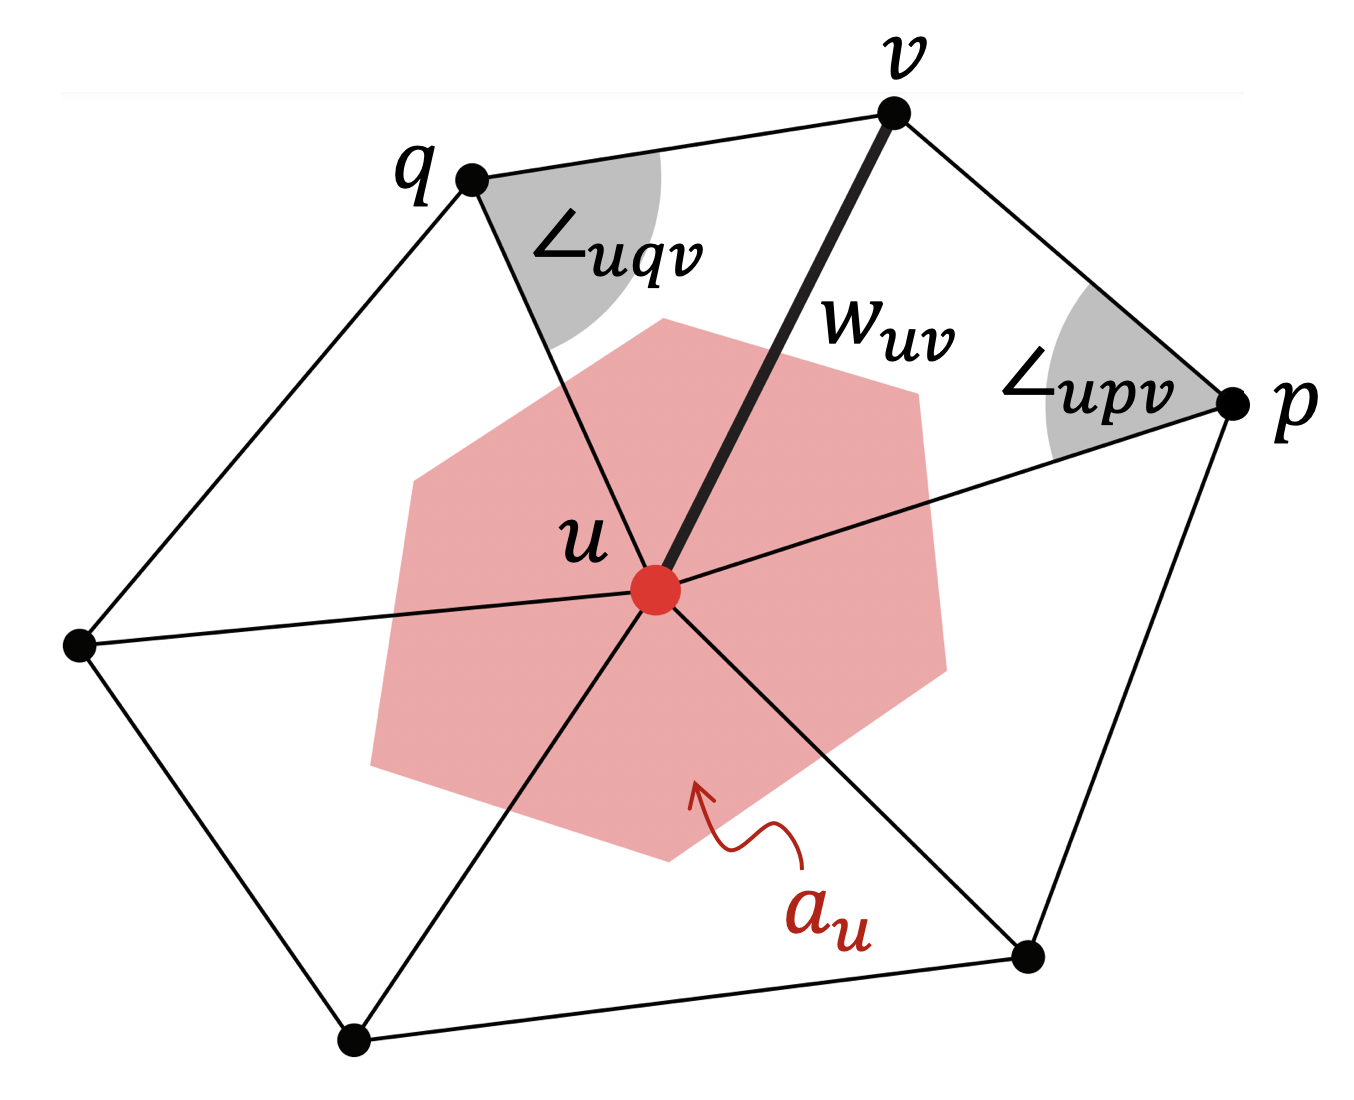
\includegraphics[width=\linewidth]{figures/cotan.png}
The earliest use of this formula dates back to the PhD thesis of \cite{macneal1949solution}, who developed it to solve PDEs on the Caltech Electric Analog Computer.}
\begin{equation}
w_{uv} = \frac{\cot \angle_{uqv} + \cot \angle_{upv}}{2 a_u}
\label{eq:cotan}
\end{equation}
where $\angle_{uqv}$ and $\angle_{upv}$ are the two angles in the triangles $(u,q,v)$ and $(u,p,v)$ opposite the shared edge $(u,v)$, and $a_u$ is the local area element, typically computed as the area of the polygon constructed upon the barycenters of the triangles $(u,p,q)$ sharing the node $u$ and given by
%
$a_u = \frac{1}{3}\sum_{v,q : (u,v,q) \in \mathcal{F}} a_{uvq}$.


The cotangent Laplacian can be shown to have multiple convenient properties (see e.g. \cite{wardetzky2007discrete}): it is a {\em positive-semidefinite} matrix, $\boldsymbol{\Delta} \succcurlyeq 0$ and thus has non-negative eigenvalues $\lambda_1 \leq \hdots \leq \lambda_n$ that can be regarded as an analogy of frequency, it is symmetric and thus has orthogonal eigenvectors, and it is {\em local} (i.e., the value of $(\boldsymbol{\Delta}\mathbf{X})_u$ depends only on 1-hop neighbours, $\mathcal{N}_u$).
%
Perhaps the most important property is the convergence of the cotangent mesh Laplacian matrix $\boldsymbol{\Delta}$ to the continuous operator $\Delta$ when the mesh is infinitely refined \citep{wardetzky2008convergence}.  Equation~(\ref{eq:cotan}) constitutes thus an appropriate {\em discretisation}\marginnote{Some technical conditions must be imposed on the refinement, to avoid e.g. triangles becoming pathological. One such example is a bizarre triangulation of the cylinder known in German as the {\em Schwarzscher Stiefel} (Schwarz's boot) or in English literature as the `Schwarz lantern', proposed in 1880 by Hermann Schwarz, a German mathematician known from the Cauchy-Schwarz inequality fame. } of the Laplacian operator defined on Riemannian manifolds in Section~\ref{sec:manifolds}. 


While one expects the Laplacian to be intrinsic, this is not very obvious from equation~(\ref{eq:cotan}), and it takes some effort to % this construction is intrinsic: one can in fact
express the cotangent weights entirely in terms of the discrete metric $\ell$ as 
$$
w_{uv} = \frac{-\ell^2_{uv} + \ell^2_{vq} + \ell^2_{uq} }{8 a_{uvq}} + 
\frac{-\ell^2_{uv} + \ell^2_{vp} + \ell^2_{up} }{8 a_{uvp}}
$$
%
where the area of the triangles $a_{ijk}$ is given as  
$$
a_{uvq} = \sqrt{s_{uvq} (s_{uvq} - \ell_{uv}) (s_{uvq} - \ell_{vq}) (s_{uvq} - \ell_{uq}) }
$$
using {\em Heron's semiperimeter formula} with 
%$s_{ijk} = \frac{1}{2}(\ell_{ij} + \ell_{ik} + \ell_{jk})$. 
$s_{uvq} = \frac{1}{2}(\ell_{uv} + \ell_{uq} + \ell_{vq})$. 
%
%
This endows the Laplacian (and any quantities associated with it, such as its eigenvectors and eigenvalues) with {\em isometry invariance}, a property for which it is so loved in geometry processing and computer graphics (see an excellent review by \cite{wang2019intrinsic}): any deformation of the mesh that does not affect the metric $\ell$ (does not `stretch' or `squeeze' the edges of the mesh) does not change the Laplacian.



Finally, as we already noticed,\marginnote{
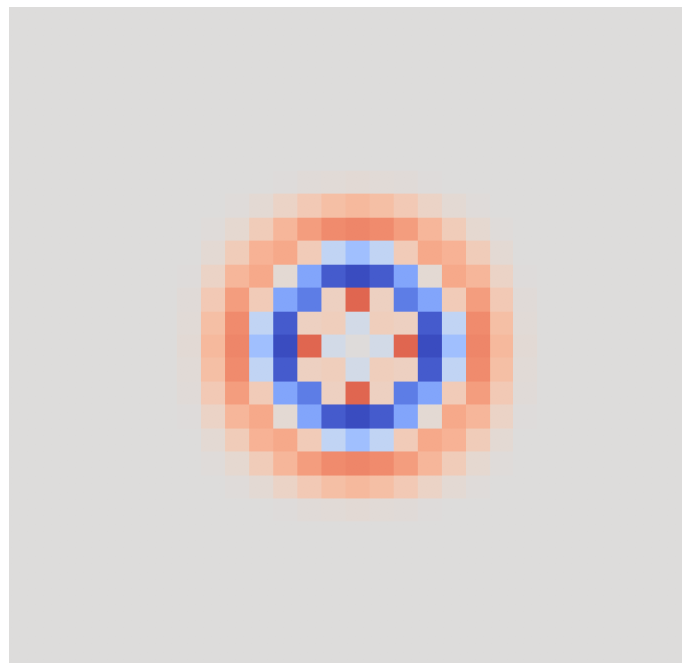
\includegraphics[width=0.9\linewidth]{figures/isotropic.png}
Laplacian-based filters are isotropic. In the plane, such filters have radial symmetry. 
} the definition of the Laplacian~(\ref{eq:cotan}) is invariant to the permutation of nodes in $\mathcal{N}_u$, as it involves aggregation in the form of summation. 
%
While on general graphs this is a necessary evil due to the lack of canonical ordering of neighbours, on meshes we can order the 1-hop neighbours according to some orientation (e.g., clock-wise), and the only ambiguity is the selection of the first node. Thus, instead of any possible permutation we need to account for {\em cyclic shifts} (rotations), which intuitively corresponds to the ambiguity arising from $\mathrm{SO}(2)$ gauge transformations discussed in Section~\ref{sec:gauges}. 
%
For a fixed gauge, it is possible to define an {\em anisotropic Laplacian} that is sensitive to local directions and amounts to changing the metric or the weights $w_{uv}$. 
%
Constructions of this kind were used to design shape descriptors by \cite{andreux2014anisotropic,boscaini2016anisotropic} and in early Geometric Deep Learning architectures on meshes by \cite{boscaini2016learning}. 



\paragraph{Spectral analysis on meshes}
%
The orthogonal eigenvectors $\boldsymbol{\Phi} = (\boldsymbol{\varphi}_1, \hdots, \boldsymbol{\varphi}_n)$ diagonalising the  Laplacian matrix ($\boldsymbol{\Delta} = \boldsymbol{\Phi} \boldsymbol{\Lambda} \boldsymbol{\Phi}^\top$, where $\boldsymbol{\Lambda} = \mathrm{diag}(\lambda_1, \hdots, \lambda_n)$ is the diagonal matrix of Laplacian eigenvalues), are used as the non-Euclidean analogy of the Fourier basis, allowing to perform spectral convolution on the mesh as the product of the respective Fourier transforms, 
$$
\mathbf{X} \star \boldsymbol{\theta} = 
\boldsymbol{\Phi} \, \mathrm{diag}(\boldsymbol{\Phi}^\top \boldsymbol{\theta}) (\boldsymbol{\Phi}^\top \mathbf{X}) 
=
\boldsymbol{\Phi}\, \mathrm{diag}(\hat{\boldsymbol{\theta}}) \hat{\mathbf{X}},
$$
%
where the filter $\hat{\boldsymbol{\theta}}$ is designed directly in the Fourier domain.  
%
Again, nothing in this formula is specific to meshes, and one can use the Laplacian matrix of a generic (undirected) graph.\marginnote{The fact that the graph is assumed to be undirected is important: in this case the Laplacian is symmetric and has orthogonal eigenvectors.}
%
%
It is tempting to exploit this spectral definition of convolution to generalise CNNs to graphs, which in fact was done by one of the authors of this text, \cite{bruna2013spectral}. 
%
However, it appears that the non-Euclidean Fourier transform 
is extremely sensitive to even minor perturbations of the underlying mesh or graph (see Figure~\ref{fig:mesh_horses} in Section~\ref{sec:manifolds}) and thus can only be used when one has to deal with different signals on a {\em fixed} domain, but not when one wishes to generalise across {\em different domains}. 
%
Unluckily, many computer graphics and vision problems fall into the latter category, where one trains a neural network on one set of 3D shapes (meshes) and test on a different set, making the Fourier transform-based approach inappropriate.  

%is given a training set of 3D shapes (meshes) and a different test, the generalisation across domains 



As noted in Section~\ref{sec:manifolds}, it is preferable to use spectral filters of the form~(\ref{eqn:conv_spec}) applying some transfer function $\hat{p}(\lambda)$ to the Laplacian matrix, 
$$
\hat{p}(\boldsymbol{\Delta})\mathbf{X} = \boldsymbol{\Phi} \hat{p}(\boldsymbol{\Lambda})\boldsymbol{\Phi}^\top\mathbf{X} 
= \boldsymbol{\Phi}\, \mathrm{diag}(\hat{p}(\lambda_1), \hdots, \hat{p}(\lambda_n)) \hat{\mathbf{X}}. 
$$
%
%which can be parametrised with a small number of parameters and computer efficiently. 
%
When $\hat{p}$ can be expressed in terms of matrix-vector products, the eigendecomposition of the $n\times n$ matrix $\boldsymbol{\Delta}$ \marginnote{In the general case, the complexity of eigendecomposition is $\mathcal{O}(n^3)$.} can be avoided altogether.  
%
For example, \cite{defferrard2016convolutional} used  {\em polynomials} of degree $r$ as filter functions, %in which case the filter is expressed as 
$$
\hat{p}(\boldsymbol{\Delta})\mathbf{X} = \sum_{k=0}^r \alpha_k \boldsymbol{\Delta}^k \mathbf{X}  = \alpha_0 \mathbf{X} + \alpha_1 \boldsymbol{\Delta} \mathbf{X}  + \hdots + \alpha_r \boldsymbol{\Delta}^r \mathbf{X}, 
$$
amounting to the multiplication of the $n\times d$ feature matrix $\mathbf{X}$ by the $n\times n$ Laplacian matrix $r$ times. Since the Laplacian is typically sparse (with $\mathcal{O}(|\mathcal{E}|)$ non-zero elements) \marginnote{Meshes are nearly-regular graphs, with each node having $\mathcal{O}(1)$ neighbours, resulting in $\mathcal{O}(n)$ non-zeros in $\boldsymbol{\Delta}$.  }
%
this operation has low complexity of $\mathcal{O}(|\mathcal{E}|dr)\sim \mathcal{O}(|\mathcal{E}|)$. 
%
Furthermore, since the Laplacian is local,  %(i.e., the value of $(\boldsymbol{\Delta}\mathbf{X})_i$ depends only on 1-hop neighbours, $\mathcal{N}_i$), 
a polynomial filter of degree $r$ is localised in $r$-hop neighbourhood. 


However, this exact property comes at a disadvantage when dealing with meshes, since the actual support of the filter (i.e., the radius it covers) depends on the {\em resolution} of the mesh. 
%
One has to bear in mind that meshes arise from the discretisation of some underlying continuous surface, and one may have two different meshes $\mathcal{T}$ and $\mathcal{T}'$ representing {\em the same object}. \marginnote{    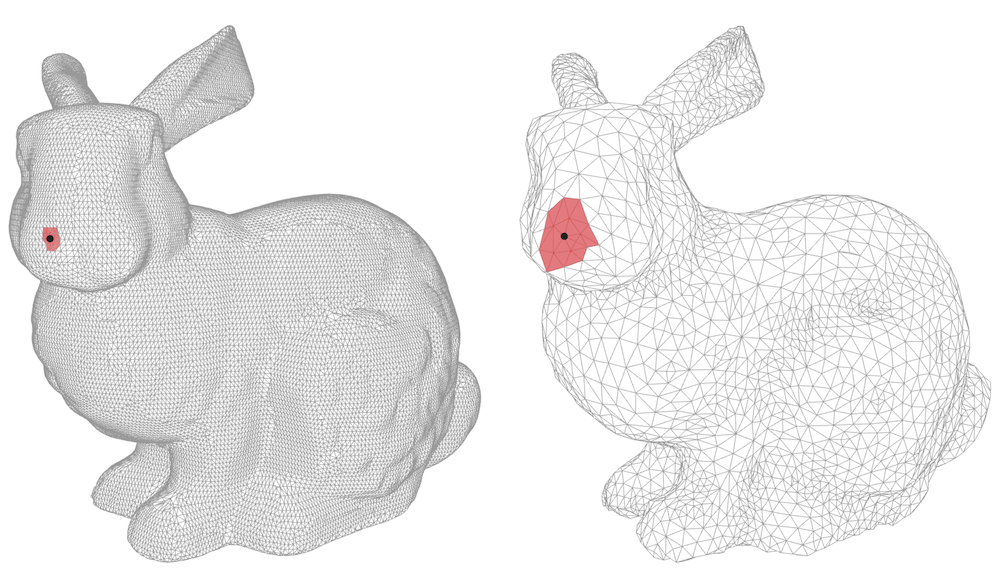
\includegraphics[width=\linewidth]{figures/mesh_res.png}\\
Two-hop neighbourhoods on meshes of different resolution. } 
%
In a finer mesh, one might have to use larger neighbourhoods (thus, larger degree $r$ of the filter) than in a coarser one. 
%

For this reason, in computer graphics applications it is more common to use {\em rational filters}, since they are  resolution-independent. There are many ways to define such filters (see, e.g. \cite{patane2020fourier}), the most common being as a polynomial of some  rational function, e.g., $\frac{\lambda-1}{\lambda+1}$. 
%
More generally, one can use a complex function, such as the {\em Cayley transform} $\frac{\lambda - \mi}{ \lambda + \mi}$ that maps the real line into the unit circle in the complex plane. \marginnote{Cayley transform is a particular case of a {\em M{\"o}bius transformation}. When applied to the Laplacian (a positive-semindefinite matrix), it maps its non-negative eigenvalues to the complex  half-circle. }
%
\cite{levie2018cayleynets} used spectral filters expressed as {\em Cayley polynomials}, real rational functions with complex coefficients $\alpha_l \in \mathbb{C}$,   
$$
\hat{p}(\lambda) = \mathrm{Re} \left(  \sum_{l=0}^r 
\alpha_l \left( \frac{\lambda - \mi}{ \lambda + \mi}
\right)^{l}
\right).
$$
%
When applied to matrices, the computation of the Cayley polynomial requires matrix inversion, 
$$
\hat{p}(\boldsymbol{\Delta}) = \mathrm{Re} \left(  \sum_{l=0}^r
\alpha_l (\boldsymbol{\Delta} - \mi\mathbf{I})^{l} (\boldsymbol{\Delta} + \mi\mathbf{I})^{-l}
\right),\marginnote{In signal processing, polynomial filters are termed {\em finite impulse response} (FIR), whereas rational filters are {\em infinite impulse response} (IIR).}
$$
which can be carried out approximately with linear complexity. 
%
Unlike polynomial filters, rational filters do not have a local support, but have exponential decay %and thus localised 
\citep{levie2018cayleynets}.  
%
A crucial difference compared to the direct computation of the Fourier transform is that polynomial and rational filters are stable under approximate isometric deformations of the underlying graph or mesh -- various results of this kind were shown e.g. by \cite{levie2018cayleynets,levie2019transferability,gama2020stability,kenlay2021interpretable}. 



%\paragraph{Anisotropic Laplacians}






\paragraph{Meshes as operators and Functional maps}


The paradigm of functional maps suggests thinking of meshes as {\em operators}. As we will show, this allows obtaining more interesting types of invariance exploiting the additional structure of meshes.  
%
For the purpose of our discussion, assume the mesh $\mathcal{T}$ is constructed upon embedded nodes with coordinates $\mathbf{X}$. 
%
If we construct an intrinsic operator like the Laplacian, it can be shown that it encodes completely the structure of the mesh, and one can recover the mesh (up to its isometric embedding, as shown by \cite{zeng2012discrete}). 
%
This is also true for some other operators (see e.g. \cite{boscaini2015shape,corman2017functional,chern2018shape}), so we will assume a general operator, or $n\times n$ matrix  $\mathbf{Q}(\mathcal{T}, \mathbf{X})$, as a representation of our mesh.  


In this view, the discussion of Section~\ref{sec:proto-graphs} of learning functions of the form   $f(\mathbf{X},\mathcal{T})$ %(as we had in our discussion on graphs in Section~\ref{sec:proto-graphs}) 
can be rephrased 
as learning functions of the form $f(\mathbf{Q})$. 
%
Similar to graphs and sets, the nodes of meshes also have no canonical ordering, i.e., functions on meshes must satisfy the permutation invariance or equivariance conditions, 
\begin{eqnarray*}
f(\mathbf{Q}) &=& f(\mathbf{P}\mathbf{Q}\mathbf{P}^\top) \\
%
\mathbf{P}\mathbf{F}(\mathbf{Q}) &=& \mathbf{F}(\mathbf{P}\mathbf{Q}\mathbf{P}^\top)
\end{eqnarray*}
% 
for any permutation matrix $\mathbf{P}$. 
%Conceptually, the permutation matrix can be considered as {\em correspondence} between two isomorphic meshes, i.e., meshes with the same number of nodes and identical connectivity. 
%
%
However, compared to general graphs we now have more structure: we can assume that our mesh arises from the discretisation of some underlying continuous surface $\Omega$. It is thus possible to have a different mesh  $\mathcal{T}'=(\mathcal{V}',\mathcal{E}',\mathcal{F}')$ with $n'$ nodes and coordinates $\mathbf{X}'$ representing the same object $\Omega$ as $\mathcal{T}$. 
%\marginnote{It is convenient to think of $\mathcal{T}'$ as a {\em remeshing} of $\mathcal{T}$.}  
%
%
Importantly, the meshes $\mathcal{T}$ and $\mathcal{T}'$ can have a different connectivity structure and even different number of nodes ($n'\neq n$). Therefore, we cannot think of these meshes as isomorphic graphs with mere reordering of nodes and consider the permutation matrix $\mathbf{P}$ as correspondence between them. 


Functional maps were introduced by \cite{ovsjanikov2012functional} as a generalisation of the notion of correspondence to such settings, replacing the correspondence between {\em points} on two domains (a map $\eta : \Omega \rightarrow \Omega'$) with correspondence between {\em functions} (a map $\mathbf{C}:\mathcal{X}(\Omega) \rightarrow \mathcal{X}(\Omega')$, see  Figure~\ref{fig:func_maps}). 
%
A {\em functional map} is a linear operator 
$\mathbf{C}$, represented as a matrix $n'\times n$,  establishing correspondence between signals $\mathbf{x}'$
%\in \mathcal{X}(\mathcal{T}')$  
%defined on the nodes of the mesh of $\mathcal{T}'$ 
and $\mathbf{x}$ % \in \mathcal{X}(\mathcal{T})$ as 
on the respective domains as 
%defined on the nodes of the mesh of $\mathcal{T}$ as 
$$
\mathbf{x}' = \mathbf{C}\mathbf{x}.\marginnote{
In most cases the functional map is implemented in the spectral domain, as a $k\times k$ map $\hat{\mathbf{C}}$ between the Fourier coefficients,
$
\mathbf{x}' = \boldsymbol{\Phi}'\hat{\mathbf{C}}\boldsymbol{\Phi}^\top\mathbf{x},
$
where $\boldsymbol{\Phi}$ and $\boldsymbol{\Phi}'$ are the respective $n\times k$ and $n'\times k$ matrices of the (truncated) Laplacian eigenbases, with $k\ll n,n'$. 
}
$$
%
%
%\michael{[TODO: Typically, $C$ is constructed in the Fourier domain - explain how. We want to have $C$ square to avoid problems with dimensions]}
\cite{rustamov2013map} showed that in order to guarantee {\em area-preserving} mapping, the functional map must be orthogonal, $\mathbf{C}^\top \mathbf{C} = \mathbf{I}$, i.e., be an element of the orthogonal group $\mathbf{C} \in \mathrm{O}(n)$. In this case, we can invert the map using $\mathbf{C}^{-1} = \mathbf{C}^\top$. 


\begin{figure}[h!]
    \centering
    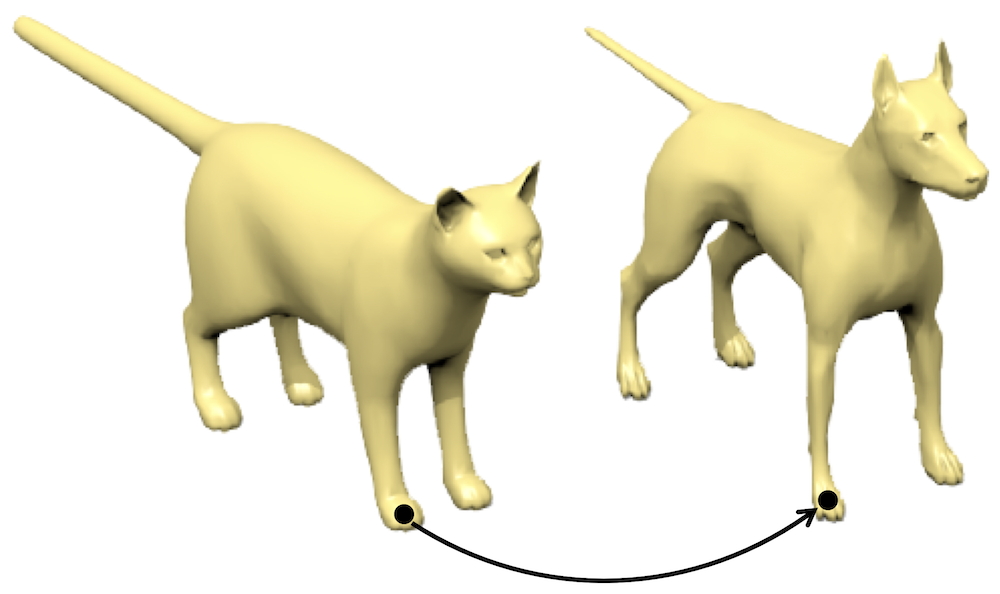
\includegraphics[width=0.45\linewidth]{figures/map_point.png}\hspace{5mm}    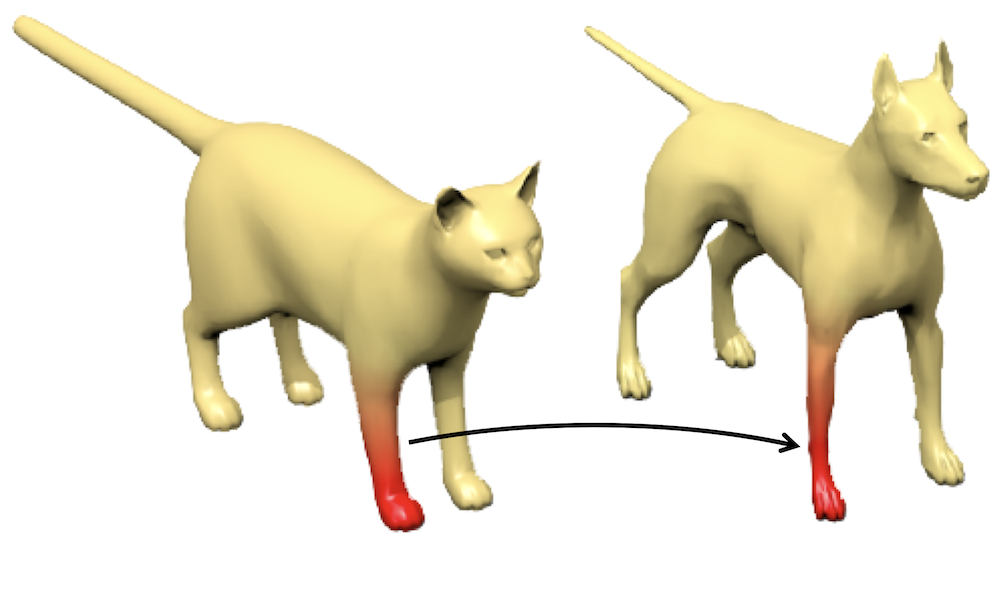
\includegraphics[width=0.45\linewidth]{figures/map_func.png}
    \caption{Pointwise map (left) vs functional map (right).   
    }
    \label{fig:func_maps}
\end{figure}%


The functional map also establishes a relation between the operator representation of meshes, 
$$
\mathbf{Q}' = \mathbf{C} \mathbf{Q} \mathbf{C}^\top, \quad \quad \mathbf{Q} = \mathbf{C}^\top \mathbf{Q}' \mathbf{C}, 
$$
%
which we can interpret as follows: given an operator representation $\mathbf{Q}$ of $\mathcal{T}$ and a functional map $\mathbf{C}$, we can construct its representation $\mathbf{Q}'$ of $\mathcal{T}'$ by first mapping the signal from $\mathcal{T}'$ to $\mathcal{T}$ (using $\mathbf{C}^\top$), applying the operator $\mathbf{Q}$, and then mapping back to $\mathcal{T}'$ (using $\mathbf{C}$)\marginnote{Note that we read these operations \emph{right-to-left}. }
%, i.e. we assume left-multiplication with a signal on $\mathcal{T}'$.}. 
%
This leads us to a more general class of {\em remeshing  invariant} (or equivariant) functions on meshes, satisfying 
%
\begin{eqnarray*}
f(\mathbf{Q}) &=& f(\mathbf{C}\mathbf{Q}\mathbf{C}^\top) = f(\mathbf{Q}')\\
%
\mathbf{C}\mathbf{F}(\mathbf{Q}) &=& \mathbf{F}(\mathbf{C}\mathbf{Q}\mathbf{C}^\top) = \mathbf{F}(\mathbf{Q}')
\end{eqnarray*}
% 
for any $\mathbf{C} \in \mathrm{O}(n)$. 
%
It is easy to see that the previous setting of permutation invariance and equivariance is a particular case,  \marginnote{This follows from the orthogonality of permutation matrices, $\mathbf{P}^\top \mathbf{P} = \mathbf{I}$.}
which can be thought of as a trivial remeshing in which only the order of nodes is changed.


\cite{wang2019learning} showed that given an eigendecomposition of the operator $\mathbf{Q} = \mathbf{V}\boldsymbol{\Lambda}\mathbf{V}^\top$, any remeshing invariant (or equivariant) function can be expressed as 
%
%
$f(\mathbf{Q}) = f(\boldsymbol{\Lambda})$ and 
%
$\mathbf{F}(\mathbf{Q}) = \mathbf{V} \mathbf{F}(\boldsymbol{\Lambda})$, 
%
or in other words, remeshing-invariant functions {\em involve only the spectrum of} $\mathbf{Q}$. 
%
%
Indeed, functions of Laplacian eigenvalues have been proven in practice to be robust to surface discretisation and perturbation, explaining the popularity of spectral constructions based on Laplacians in computer graphics, as well as in deep learning on graph \citep{defferrard2016convolutional,levie2018cayleynets}. 
%
%In graph deep learning literature, architectures such as ChebNet \citep{defferrard2016convolutional} and CayleyNet \citep{levie2018cayleynets} explicitly learn functions of Laplacian eigenvalues. 
%
%
Since this result refers to a generic operator $\mathbf{Q}$, multiple choices are available besides the ubiquitous Laplacian -- notable examples include the Dirac \citep{liu2017dirac,kostrikov2018surface} or Steklov \citep{wang2018steklov} operators, as well as learnable parametric operators \citep{wang2019learning}. 


%\michael{The degree of freedom we have is the operator itself - which leads to learnable operators.}

%\joan{We might want to mention extrinsic models that build anisotropy based on the Dirac Operator rather than the Laplace operator; Crane et al, and our Surface Network paper}
%\joan{This section clearly needs to branch out into its own chapter. }


